\documentclass[12pt,oneside]{book}

%%%%%%%%%%%%%%%%%%%%%%%%%%%%%%%%%%%%%%%%%%%%%%%%%%%%%%%%%%%%%%%%%%%%%%%%%%%%%%%%%%%%%%%%%%%%%%%%%%%
%                                                                                                 %
% The mathematical style of these documents follows                                               %
%                                                                                                 %
% A. Thompson and B.N. Taylor. The NIST Guide for the Use of the International System of Units.   %
%    NIST Special Publication 881, 2008.                                                          %
%                                                                                                 %
% http://www.nist.gov/pml/pubs/sp811/index.cfm                                                    %
%                                                                                                 %
%%%%%%%%%%%%%%%%%%%%%%%%%%%%%%%%%%%%%%%%%%%%%%%%%%%%%%%%%%%%%%%%%%%%%%%%%%%%%%%%%%%%%%%%%%%%%%%%%%%

% $Date: 2013-11-26 10:43:59 -0500 (Tue, 26 Nov 2013) $
% $Revision: 17538 $
% $Author: gforney $

%%%%%%%%%%%%%%%%%%%%%%%%%%%%%%%%%%%%%%%%%%%%%%%%%%%%%%%%%%%%%%%%%%%%%%%%%%%%%%%%%%%%%%%%%%%%%%%%%%%
%                                                                                                 %
% The mathematical style of these documents follows                                               %
%                                                                                                 %
% A. Thompson and B.N. Taylor. The NIST Guide for the Use of the International System of Units.   %
%    NIST Special Publication 881, 2008.                                                          %
%                                                                                                 %
% http://www.nist.gov/pml/pubs/sp811/index.cfm                                                    %
%                                                                                                 %
%%%%%%%%%%%%%%%%%%%%%%%%%%%%%%%%%%%%%%%%%%%%%%%%%%%%%%%%%%%%%%%%%%%%%%%%%%%%%%%%%%%%%%%%%%%%%%%%%%%

% Packages which force the use of better TeX coding
% Mostly from http://tex.stackexchange.com/q/19264
%%\RequirePackage[l2tabu, orthodox]{nag}
%%\usepackage{fixltx2e}
%\usepackage{isomath} % Disabled for the moment because it changes the syntax for bold and roman Greek math symbols
%%\usepackage[all,warning]{onlyamsmath}
%\usepackage{strict} % Commented out for now because it is uncommon. A copy of style.sty is in Manuals/LaTeX_Style_Files/.

\usepackage{times,mathptmx}
\usepackage[pdftex]{graphicx}
\usepackage{tabularx,ragged2e,booktabs,caption}
\usepackage{multirow}
\usepackage{pdfsync}
\usepackage{tikz}
\usepackage{pgfplots}
%\pgfplotsset{compat=1.7}
\usepackage{tocloft}
\usepackage{color}
\usepackage{amsmath}
\definecolor{linknavy}{rgb}{0,0,0.50196}
\definecolor{linkred}{rgb}{1,0,0}
\definecolor{linkblue}{rgb}{0,0,1}
\usepackage{float}
\usepackage{caption}
\usepackage{graphpap}
\usepackage{rotating}
\usepackage{graphicx}
\usepackage{geometry}
\usepackage{relsize}
\usepackage{longtable}
\usepackage{lscape}
\usepackage{amssymb}
\usepackage{makeidx} % Create index at end of document
\usepackage[nottoc,notlof,notlot]{tocbibind} % Put the bibliography and index in the ToC
\usepackage{lastpage} % Automatic last page number reference.
\usepackage[T1]{fontenc}
\usepackage{enumerate}
\usepackage{upquote}
\usepackage{moreverb}
\usepackage{xfrac}
\usepackage{cite}

\newcommand{\nopart}{\expandafter\def\csname Parent-1\endcsname{}} % To fix table of contents in pdf.
\newcommand{\ct}{\tt\small} % eventually will be deprecated due to http://www.tex.ac.uk/cgi-bin/texfaq2html?label=2letterfontcmd
\newcommand{\textct}[1]{\texttt{\small #1}}

\usepackage{tocstyle} % Fix table of contents sections from overlapping section titles
\usetocstyle{standard}
\usepackage{siunitx}
\sisetup{
    detect-all = true,
    input-decimal-markers = {.},
    input-ignore = {,},
    inter-unit-product = \ensuremath{{}\cdot{}},
    multi-part-units = repeat,
    number-unit-product = \text{~},
    per-mode = fraction,
    separate-uncertainty = true,
}

\usepackage{listings}
\usepackage{textcomp}
\definecolor{lbcolor}{rgb}{0.96,0.96,0.96}
\lstset{
    %backgroundcolor=\color{lbcolor},
    tabsize=4,
    rulecolor=,
    language=Fortran,
        basicstyle=\footnotesize\ttfamily,
        upquote=true,
        aboveskip={\baselineskip},
        belowskip={\baselineskip},
        columns=fixed,
        extendedchars=true,
        breaklines=true,
        breakatwhitespace=true,
        frame=none,
        showtabs=false,
        showspaces=false,
        showstringspaces=false,
        identifierstyle=\ttfamily,
        keywordstyle=\color[rgb]{0,0,0},
        commentstyle=\color[rgb]{0,0,0},
        stringstyle=\color[rgb]{0,0,0},
}

\usepackage[pdftex,
        colorlinks=true,
        urlcolor=linkblue,     % \href{...}{...} external (URL)
        citecolor=linkred,     % citation number colors
        linkcolor=linknavy,    % \ref{...} and \pageref{...}
        pdfproducer={pdflatex},
        pdfpagemode=UseNone,
        bookmarksopen=true,
        plainpages=false,
        verbose]{hyperref}

% The Following commented code makes the ``Draft'' watermark on each page.
%\usepackage{eso-pic}
%\usepackage{type1cm}
%\makeatletter
%   \AddToShipoutPicture{
%     \setlength{\@tempdimb}{.5\paperwidth}
%     \setlength{\@tempdimc}{.5\paperheight}
%     \setlength{\unitlength}{1pt}
%     \put(\strip@pt\@tempdimb,\strip@pt\@tempdimc){
%     \makebox(0,0){\rotatebox{45}{\textcolor[gray]{0.75}{\fontsize{8cm}\selectfont{RC6}}}}}
% }
%\makeatother

\setlength{\textwidth}{6.5in}
\setlength{\textheight}{9.0in}
\setlength{\topmargin}{0.in}
\setlength{\headheight}{0.pt}
\setlength{\headsep}{0.in}
\setlength{\parindent}{0.25in}
\setlength{\oddsidemargin}{0.0in}
\setlength{\evensidemargin}{0.0in}
\setlength{\leftmargini}{\parindent} % Controls the indenting of the "bullets" in a list
\setlength{\cftsecnumwidth}{0.45in}
\setlength{\cftsubsecnumwidth}{0.5in}
\setlength{\cftfignumwidth}{0.45in}
\setlength{\cfttabnumwidth}{0.45in}

\newcommand{\titlesigs}
{
\small
\flushright{U.S. Department of Commerce \\
{\em Penny Pritzker, Secretary} \\
\hspace{1in} \\
National Institute of Standards and Technology \\
{\em Willie May, Under Secretary of Commerce for Standards and Technology and Acting Director} }
}

% commands to use for "official" cover and title pages
% see smokeview verification guide to see how they are used

\newcommand{\headerA}[1]{
\flushright{
\fontsize{20}{24}\selectfont
\bf{NIST Special Publication #1}}
}

\newcommand{\headerB}[1]{
\flushright{
\fontsize{28}{33.6}\selectfont
\bf{#1}
}
}

\newcommand{\headerC}[1]{
\vspace{.5in}
\flushright{\fontsize{14}{16.8}\selectfont
#1}
}

\frenchspacing

\newcommand{\dod}[2]{\frac{\partial #1}{\partial #2}}
\newcommand{\DoD}[2]{\frac{\mathrm{D} #1}{\mathrm{D} #2}}
\newcommand{\dsods}[2]{\frac{\partial^2 #1}{\partial #2^2}}
\renewcommand{\d}{\,\mathrm{d}}
\newcommand{\dx}{\delta x}
\newcommand{\dy}{\delta y}
\newcommand{\dz}{\delta z}
\newcommand{\degF}{$^\circ$F}
\newcommand{\degC}{$^\circ$C}
\newcommand{\x}{x}
\newcommand{\y}{y}
\newcommand{\z}{z}
\newcommand{\dt}{\delta t}
\newcommand{\dn}{\delta n}
\newcommand{\cH}{H}
\newcommand{\hu}{u}
\newcommand{\hv}{v}
\newcommand{\hw}{w}
\newcommand{\la}{\lambda}
\newcommand{\bO}{{\Omega}}
\newcommand{\bo}{{\mathbf{\omega}}}
\newcommand{\btau}{\mathbf{\tau}}
\newcommand{\bdelta}{{\mathbf{\delta}}}
\newcommand{\sumyw}{\sum (Y_\alpha/W_\alpha)}
\newcommand{\oW}{\overline{W}}
\newcommand{\om}{\ensuremath{\omega}}
\newcommand{\omx}{\omega_x}
\newcommand{\omy}{\omega_y}
\newcommand{\omz}{\omega_z}
\newcommand{\erf}{\hbox{erf}}
\newcommand{\erfc}{\hbox{erfc}}
\newcommand{\bF}{{\mathbf{F}}}
\newcommand{\bG}{{\mathbf{G}}}
\newcommand{\bof}{{\mathbf{f}}}
\newcommand{\bq}{{\mathbf{q}}}
\newcommand{\br}{{\mathbf{r}}}
\newcommand{\bu}{{\mathbf{u}}}
\newcommand{\bx}{{\mathbf{x}}}
\newcommand{\bk}{{\mathbf{k}}}
\newcommand{\bv}{{\mathbf{v}}}
\newcommand{\bg}{{\mathbf{g}}}
\newcommand{\bn}{{\mathbf{n}}}
\newcommand{\bS}{{\mathbf{S}}}
\newcommand{\bW}{\overline{W}}
\newcommand{\dS}{d{\mathbf{S}}}
\newcommand{\bs}{{\mathbf{s}}}
\newcommand{\bI}{{\mathbf{I}}}
\newcommand{\hp}{H}
\newcommand{\trho}{\tilde{\rho}}
\newcommand{\dph}{{\delta\phi}}
\newcommand{\dth}{{\delta\theta}}
\newcommand{\tp}{\tilde{p}}
\newcommand{\bp}{\overline{p}}
\newcommand{\dQ}{\dot{Q}}
\newcommand{\dq}{\dot{q}}
\newcommand{\dbq}{\dot{\mathbf{q}}}
\newcommand{\dm}{\dot{m}}
\newcommand{\ha}{\frac{1}{2}}
\newcommand{\ft}{\frac{4}{3}}
\newcommand{\ot}{\frac{1}{3}}
\newcommand{\fofi}{\frac{4}{5}}
\newcommand{\of}{\frac{1}{4}}
\newcommand{\twth}{\frac{2}{3}}
\newcommand{\R}{R}
\newcommand{\be}{\begin{equation}}
\newcommand{\ee}{\end{equation}}
\newcommand{\RE}{\hbox{Re}}
\newcommand{\LE}{\hbox{Le}}
\newcommand{\PR}{\hbox{Pr}}
\newcommand{\PE}{\hbox{Pe}}
\newcommand{\NU}{\hbox{Nu}}
\newcommand{\SC}{\hbox{Sc}}
\newcommand{\SH}{\hbox{Sh}}
\newcommand{\WE}{\hbox{We}}
\newcommand{\COTWO}{\text{\tiny \hbox{CO}$_2$}}
\newcommand{\HTWOO}{\text{\tiny \hbox{H}$_2$\hbox{O}}}
\newcommand{\OTWO}{\text{\tiny \hbox{O}$_2$}}
\newcommand{\NTWO}{\text{\tiny \hbox{N}$_2$}}
\newcommand{\CO}{\text{\tiny \hbox{CO}}}
\newcommand{\F}{\text{\tiny \hbox{F}}}
\newcommand{\C}{\text{\tiny \hbox{C}}}
\newcommand{\Hy}{\text{\tiny \hbox{H}}}
\newcommand{\So}{\text{\tiny \hbox{S}}}
\newcommand{\M}{\text{\tiny \hbox{M}}}
\newcommand{\xx}{\text{\tiny \hbox{x}}}
\newcommand{\yy}{\text{\tiny \hbox{y}}}
\newcommand{\zz}{\text{\tiny \hbox{z}}}
\newcommand{\smvlines}{115~000}

\newcommand{\calH}{\mathcal{H}}
\newcommand{\calR}{\mathcal{R}}

\newcommand{\dif}{\mathrm{d}}
\newcommand{\Div}{\nabla\cdot}
\newcommand{\D}{\mbox{D}}
\newcommand{\mhalf}{\mbox{$\frac{1}{2}$}}
\newcommand{\thalf}{\mbox{\tiny $\frac{1}{2}$}}
\newcommand{\tripleprime}{{\prime\prime\prime}}
\newcommand{\ppp}{{\prime\prime\prime}}
\newcommand{\pp}{{\prime\prime}}

\newcommand{\superscript}[1]{\ensuremath{^{\textrm{\tiny #1}}}}
\newcommand{\subscript}[1]{\ensuremath{_{\textrm{\tiny #1}}}}

\newcommand{\rb}[1]{\raisebox{1.5ex}[0pt]{#1}}

\newcommand{\Ra}{$\Rightarrow$}
\newcommand{\hhref}[1]{\href{#1}{{\tt #1}}}
\newcommand{\fdsinput}[1]{{\scriptsize\verbatiminput{../../Verification/Visualization/#1}}}

\definecolor{AQUAMARINE}{rgb}{0.49804,1.00000,0.83137}
\definecolor{ANTIQUE WHITE}{rgb}{0.98039,0.92157,0.84314}
\definecolor{BEIGE}{rgb}{0.96078,0.96078,0.86275}
\definecolor{BLACK}{rgb}{0.00000,0.00000,0.00000}
\definecolor{BLUE}{rgb}{0.00000,0.00000,1.00000}
\definecolor{BLUE VIOLET}{rgb}{0.54118,0.16863,0.88627}
\definecolor{BRICK}{rgb}{0.61176,0.40000,0.12157}
\definecolor{BROWN}{rgb}{0.64706,0.16471,0.16471}
\definecolor{BURNT SIENNA}{rgb}{0.54118,0.21176,0.05882}
\definecolor{BURNT UMBER}{rgb}{0.54118,0.20000,0.14118}
\definecolor{CADET BLUE}{rgb}{0.37255,0.61961,0.62745}
\definecolor{CHOCOLATE}{rgb}{0.82353,0.41176,0.11765}
\definecolor{COBALT}{rgb}{0.23922,0.34902,0.67059}
\definecolor{CORAL}{rgb}{1.00000,0.49804,0.31373}
\definecolor{CYAN}{rgb}{0.00000,1.00000,1.00000}
\definecolor{DIMGRAY }{rgb}{0.41176,0.41176,0.41176}
\definecolor{EMERALD GREEN}{rgb}{0.00000,0.78824,0.34118}
\definecolor{FIREBRICK}{rgb}{0.69804,0.13333,0.13333}
\definecolor{FLESH}{rgb}{1.00000,0.49020,0.25098}
\definecolor{FOREST GREEN}{rgb}{0.13333,0.54510,0.13333}
\definecolor{GOLD }{rgb}{1.00000,0.84314,0.00000}
\definecolor{GOLDENROD}{rgb}{0.85490,0.64706,0.12549}
\definecolor{GRAY}{rgb}{0.50196,0.50196,0.50196}
\definecolor{GREEN}{rgb}{0.00000,1.00000,0.00000}
\definecolor{GREEN YELLOW}{rgb}{0.67843,1.00000,0.18431}
\definecolor{HONEYDEW}{rgb}{0.94118,1.00000,0.94118}
\definecolor{HOT PINK}{rgb}{1.00000,0.41176,0.70588}
\definecolor{INDIAN RED}{rgb}{0.80392,0.36078,0.36078}
\definecolor{INDIGO}{rgb}{0.29412,0.00000,0.50980}
\definecolor{IVORY}{rgb}{1.00000,1.00000,0.94118}
\definecolor{IVORY BLACK}{rgb}{0.16078,0.14118,0.12941}
\definecolor{KELLY GREEN}{rgb}{0.00000,0.50196,0.00000}
\definecolor{KHAKI}{rgb}{0.94118,0.90196,0.54902}
\definecolor{LAVENDER}{rgb}{0.90196,0.90196,0.98039}
\definecolor{LIME GREEN}{rgb}{0.19608,0.80392,0.19608}
\definecolor{MAGENTA}{rgb}{1.00000,0.00000,1.00000}
\definecolor{MAROON}{rgb}{0.50196,0.00000,0.00000}
\definecolor{MELON}{rgb}{0.89020,0.65882,0.41176}
\definecolor{MIDNIGHT BLUE}{rgb}{0.09804,0.09804,0.43922}
\definecolor{MINT}{rgb}{0.74118,0.98824,0.78824}
\definecolor{NAVY}{rgb}{0.00000,0.00000,0.50196}
\definecolor{OLIVE}{rgb}{0.50196,0.50196,0.00000}
\definecolor{OLIVE DRAB}{rgb}{0.41961,0.55686,0.13725}
\definecolor{ORANGE}{rgb}{1.00000,0.50196,0.00000}
\definecolor{ORANGE RED}{rgb}{1.00000,0.27059,0.00000}
\definecolor{ORCHID}{rgb}{0.85490,0.43922,0.83922}
\definecolor{PINK}{rgb}{1.00000,0.75294,0.79608}
\definecolor{POWDER BLUE}{rgb}{0.69020,0.87843,0.90196}
\definecolor{PURPLE}{rgb}{0.50196,0.00000,0.50196}
\definecolor{RASPBERRY}{rgb}{0.52941,0.14902,0.34118}
\definecolor{RED}{rgb}{1.00000,0.00000,0.00000}
\definecolor{ROYAL BLUE}{rgb}{0.25490,0.41176,0.88235}
\definecolor{SALMON}{rgb}{0.98039,0.50196,0.44706}
\definecolor{SANDY BROWN}{rgb}{0.95686,0.64314,0.37647}
\definecolor{SEA GREEN}{rgb}{0.32941,1.00000,0.62353}
\definecolor{SEPIA}{rgb}{0.36863,0.14902,0.07059}
\definecolor{SIENNA}{rgb}{0.62745,0.32157,0.17647}
\definecolor{SILVER}{rgb}{0.75294,0.75294,0.75294}
\definecolor{SKY BLUE}{rgb}{0.52941,0.80784,0.92157}
\definecolor{SLATEBLUE}{rgb}{0.41569,0.35294,0.80392}
\definecolor{SLATE GRAY}{rgb}{0.43922,0.50196,0.56471}
\definecolor{SPRING GREEN}{rgb}{0.00000,1.00000,0.49804}
\definecolor{STEEL BLUE}{rgb}{0.27451,0.50980,0.70588}
\definecolor{TAN}{rgb}{0.82353,0.70588,0.54902}
\definecolor{TEAL}{rgb}{0.00000,0.50196,0.50196}
\definecolor{THISTLE}{rgb}{0.84706,0.74902,0.84706}
\definecolor{TOMATO }{rgb}{1.00000,0.38824,0.27843}
\definecolor{TURQUOISE}{rgb}{0.25098,0.87843,0.81569}
\definecolor{VIOLET}{rgb}{0.93333,0.50980,0.93333}
\definecolor{VIOLET RED}{rgb}{0.81569,0.12549,0.56471}
\definecolor{WHITE}{rgb}{1.00000,1.00000,1.00000}
\definecolor{YELLOW}{rgb}{1.00000,1.00000,0.00000}

\pgfplotsset{
	colormap={blackwhite}{[5pt]
		rgb255(0pt)=(0,0,255); 
		rgb255(100pt)=(0,255,255); 
		rgb255(200pt)=(0,255,0); 
		rgb255(300pt)=(255,255,0); 
		rgb255(400pt)=(255,0,0)
	},
} % defines smokeview colorbar


\floatstyle{boxed}
\newfloat{notebox}{H}{lon}
\newfloat{warning}{H}{low}

% Set default longtable alignment
\setlength\LTleft{0pt}
\setlength\LTright{0pt}


% Load extra packages
\usepackage{placeins}


% Rename chapter headings
\renewcommand{\chaptername}{Section}
\renewcommand{\bibname}{References}

% Math shortcuts
\renewcommand{\sb}[1]{_\mathrm{#1}}
\renewcommand{\C}{\mbox{C}}
\renewcommand{\H}{\mbox{H}}
\renewcommand{\O}{\mbox{O}}
\newcommand{\N}{\mbox{N}}

% Center all figures
\makeatletter
\g@addto@macro\@floatboxreset\centering
\makeatother

\begin{document}

\bibliographystyle{unsrt}
\pagestyle{empty}

\begin{minipage}[t][9in][s]{6.25in}

\begin{flushright}
\fontsize{20}{24}\selectfont
\bf{NIST Technical Note XXXX}
\end{flushright}

\headerB{
Impact of Hose Streams on Air Flows inside a Structure \\
}

\headerC{
{
\flushright{
Joseph M. Willi \\
Daniel Madrzykowski \\
Craig G. Weinschenk \\


\vspace*{2\baselineskip}

\begingroup
This publication is available free of charge from:
\hypersetup{urlcolor=black}
\href{http://dx.doi.org/10.6028/NIST.TN.XXXX}{http://dx.doi.org/10.6028/NIST.TN.XXXX}
\endgroup
}

\vfill

\flushright{


\includegraphics[width=2.in]{../../../../../Bibliography/nistident_flright_vec} \\[.3in]
}
}
}

\end{minipage}

\newpage
\hspace{5in}
\newpage

\frontmatter

\pagenumbering{roman}

\begin{minipage}[t][9in][s]{6.25in}

\begin{flushright}
\fontsize{20}{24}\selectfont
\bf{NIST Technical Note XXXX}
\end{flushright}

\headerB{
Impact of Hose Streams on Air Flows inside a Structure
}

\headerC{
\flushright{
Joseph M. Willi \\
Daniel Madrzykowski \\
Craig G. Weinschenk \\
{\em Fire Research Division \\
Engineering Laboratory} \\

\vspace*{2\baselineskip}

\begingroup
This publication is available free of charge from:
\hypersetup{urlcolor=black}
\href{http://dx.doi.org/10.6028/NIST.TN.XXXX}{http://dx.doi.org/10.6028/NIST.TN.XXXX} \\
\endgroup

\vspace*{2\baselineskip}
September 2015}}

\vfill

\flushright{
\includegraphics[width=1in]{../../../../../Bibliography/doc} }

\titlesigs

\end{minipage}

\newpage

\begin{minipage}[t][9in][s]{6.25in}

\flushright{Certain commercial entities, equipment, or materials may be identified in this \\
document in order to describe an experimental procedure or concept adequately. \\
Such identification is not intended to imply recommendation or endorsement by the \\
National Institute of Standards and Technology, nor is it intended to imply that the \\
entities, materials, or equipment are necessarily the best available for the purpose. \\
}

\vspace{3in}

\large
\flushright{\bf National Institute of Standards and Technology Technical Note XXXX \\
Natl.~Inst.~Stand.~Technol.~Tech.~Note~XX, \pageref{LastPage} pages (September 2015) \\
% http://dx.doi.org/10.6028/NIST.TN.XXXX \\
CODEN: NTNOEF }

\vspace{0.2in}

\begingroup
{\bf This publication is available free of charge from:}
\hypersetup{urlcolor=black}
\href{http://dx.doi.org/10.6028/NIST.TN.1838}{\bf http://dx.doi.org/10.6028/NIST.TN.1838} \\
\endgroup

\vfill

\hspace{1in}

\end{minipage}

\newpage

\frontmatter

\pagestyle{plain}
\pagenumbering{roman}

\cleardoublepage
\phantomsection
\addcontentsline{toc}{chapter}{Contents}
\tableofcontents

\cleardoublepage
\phantomsection
\addcontentsline{toc}{chapter}{List of Figures}
\listoffigures

\cleardoublepage
\phantomsection
\addcontentsline{toc}{chapter}{List of Tables}
\listoftables

\chapter{List of Acronyms}

\begin{tabbing}
\hspace{1.5in} \= \\
ESTC \> Delaware County Emergency Services Training Center \\
NIST \> National Institute of Standards and Technology \\
\end{tabbing}

\newpage

% \chapter{List of Symbols}
% \begin{tabbing}
% \hspace{1.5in} \= \\
% ft \> foot \\
% GPM \> gallons per minute \\
% in \> inch \\
% m \> meter \\
% \end{tabbing} 

\mainmatter


% ================
% = Introduction =
% ================
\chapter{Introduction}
\label{chap:intro}
\section{Background}
\label{sec:background}
% More hose stream studies and explanations

NIST has conducted a significant amount of research examining how ventilation affects the growth and spread of fire within structures and how the air flow to the fire may be controlled to limit or delay the growth of the fire~\cite{}. The studies have resulted in guidance to the fire service regarding ventilation tactics. However, ventilation tactics alone will not result in the complete extinguishment of the fire; fire suppression with hose streams is also needed.

Fire suppression tactics using hose streams also affect the ventilation in a structure and can impact the movement of smoke and heat through a structure as vents are made to advance the hose line or if ventilation inducing handline tactics are in practice~\cite{}. Additional research addressing the coordination of suppression tactics and the impact on ventilation is needed to complete recommendations on fire control tactics to appropriate standards, education, and training documents.

There exists a multitude of different tools, methods, and techniques used to apply water for fire suppression using hose streams. A common type of nozzle that is used to apply water during fire suppression in residential structures is a fog nozzle. Most fog nozzles contain an adjustable tip that can be rotated to produce different stream patterns and are therefore often referred to as combination nozzles. The types of streams produced by a fog nozzle are often divided into three categories based on the angle of the stream with respect to the nozzle: a straight stream typically produces an angle less than 15\SI{}{\degree}, a narrow fog stream produces an angle between 15\SI{}{\degree} and 45\SI{}{\degree}, and a wide fog stream produces an angle between 45\SI{}{\degree} to 80\SI{}{\degree}~\cite{Essentials_FF}. Increasing the angle of the stream allows for a larger area to be covered by water, thus exposing a larger water droplet surface area for heat absorption. However, increasing the angle decreases the distance reached by the stream and its penetration power and increases the potential to disrupt thermal layering increases. 
%\textit{Essentials of Fire Fighting} defines 
%https://docs.google.com/presentation/d/1hZ5DZhYXxCkcIEHNZKumH48b_Q53iM2D7asXkMYlVMM/embed?hl=en&size=l&slide=id.p39

%http://www.tft.com/literature/library/files/bfa.pdf
%Keith Royer, "Water for Fire Fighting", (Engineering Extension Service, Iowa State University, Ames, Iowa) p. 6 
In addition to the type of stream pattern used, fire suppression tactics using hose streams can differ in the method used to apply the hose stream. For example, Royer suggests using a clockwise rotation instead of a counterclockwise application pattern for the following reasons~\cite{Royer}:
\begin{enumerate} 
	\item Clockwise rotation drives most of the heated gases, smoke, and flames away from the nozzle. Counterclockwise rotation does just the opposite.
	\item Steam formed by the clockwise rotation has a violent rolling action. Counterclockwise rotation produces steam with an inactive and lazy action.
	\item A clockweise roation increases the efficiency of water and produces a faster knockdown time than counterclockwise rotation.
\end{enumerate}

\section{Objectives}
\label{sec:objectives}
This report is concerned with examining the impact of hose stream and application pattern selection on air movement inside a residential structure. Numerous experiments containing different flow path configurations were conducted to study the impact of hose stream and water application selection on ventilation in a structure. More specifically, the experiments were conducted to fulfill the following objectives:
\begin{enumerate}
	\item Determine which hose stream patterns cause significant air movement in a structure 
	\item Determine the amount of air movement induced by different stream patterns
	\item Determine the impact of different stream application patterns on the ventilation in a structure
\end{enumerate}

Three types of hose streams and four different water application patterns were studied throughout the experiments described in this report. The three types of hose stream patterns studied, pictured in Figure~\ref{fig:hose_streams}, were straight stream, narrow fog stream, and wide fog stream. Water was flowed into the structure by having the hose in a static, or fixed, position, by moving the hose line left-to-right across the room in a sweeping motion, and by rotating the hose line in both the clockwise and counterclockwise directions.

\begin{figure}[!ht]
	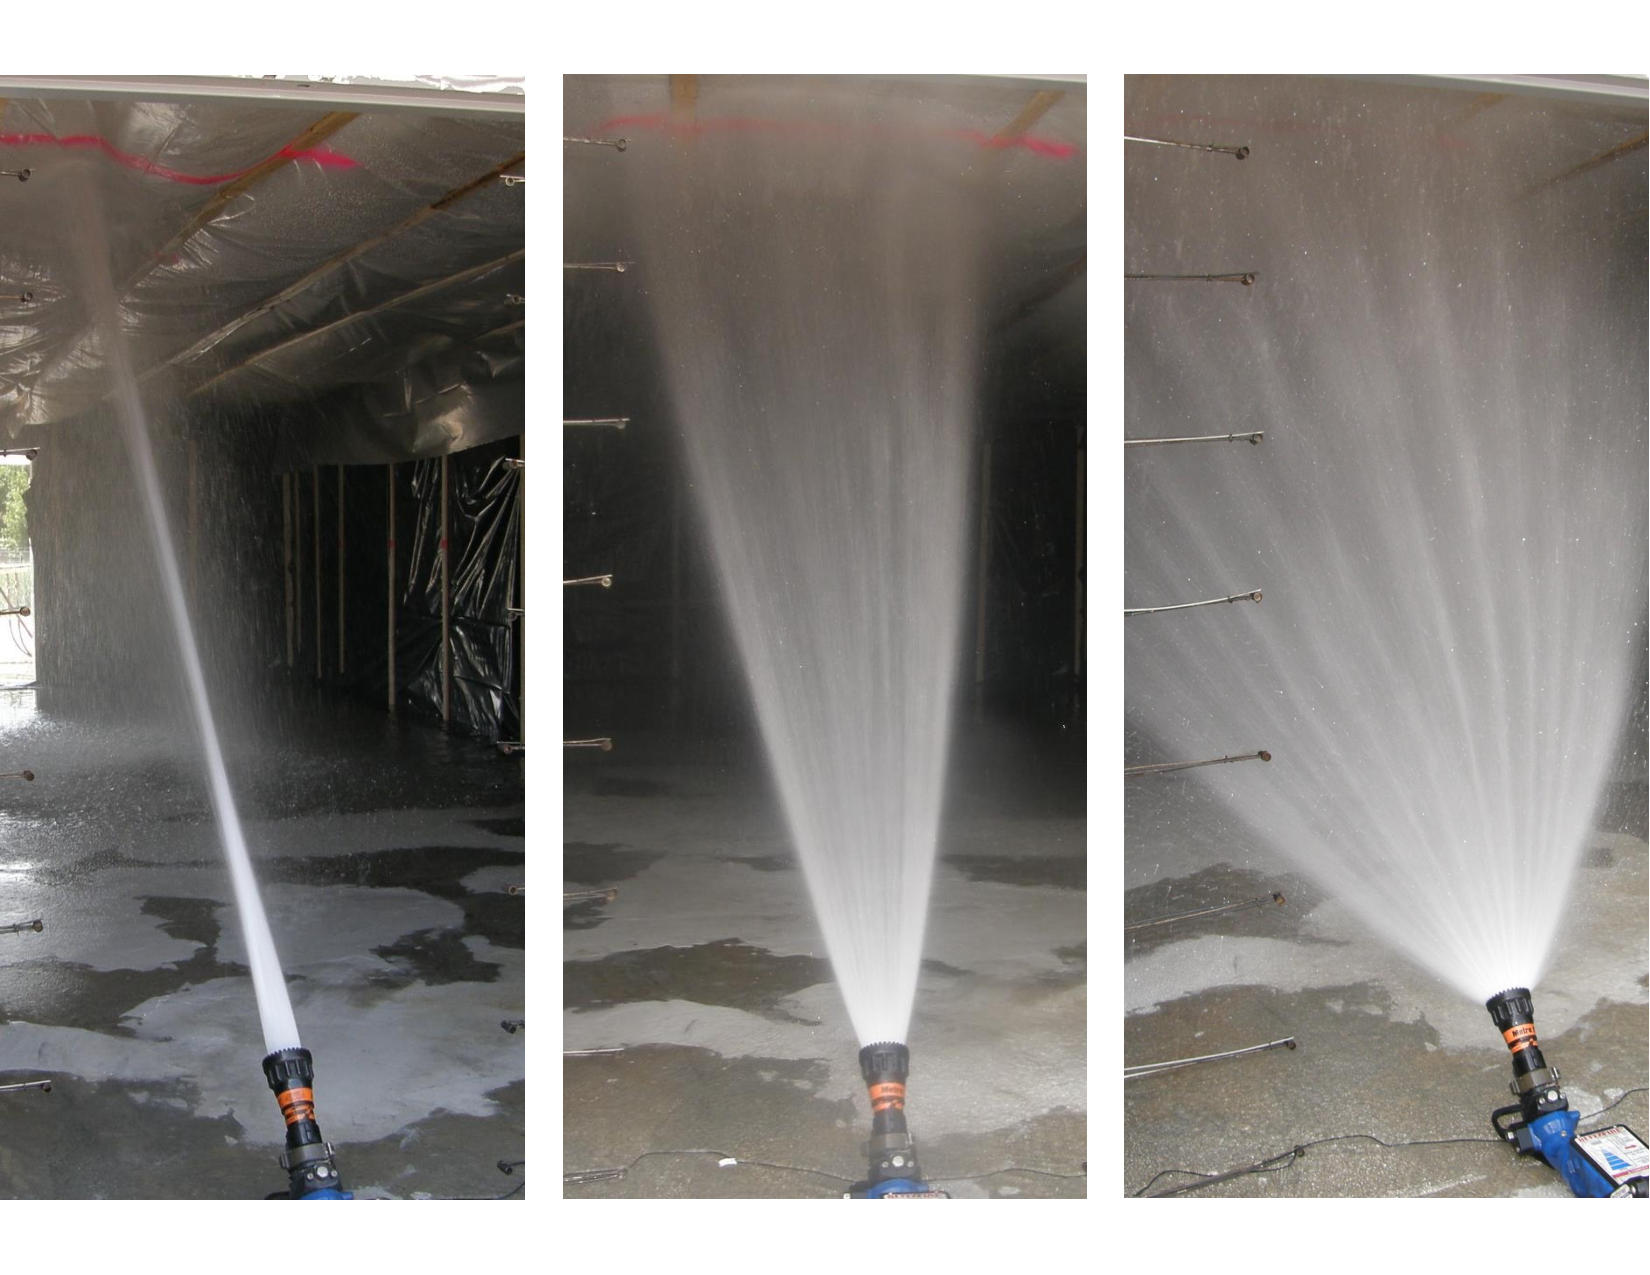
\includegraphics[width=\columnwidth]{../Figures/Pictures/hose_streams.pdf}
	\caption[Hose stream patterns used in experiments.]{The three types of stream patterns used during water flow experiments. From left to right: straight stream, narrow fog stream, and wide fog stream.}
	\label{fig:hose_streams}
\end{figure}

Additionally, a set of experiments comparing the impact of a straight stream from a combination nozzle and a solid stream from a smooth bore nozzle on air flows in a structure was conducted.

\FloatBarrier

% =========================
% = EXPERIMENTAL OVERVIEW =
% =========================
\chapter{Experimental Overview}
\label{chap:exp_overview}
To study the impact of different hose stream and application pattern selections on air movement inside a structure, various water flow experiments were conducted in two experimental structures designed to replicate typical residential structures. The experiments focused on studying the differences in amount of air movement caused by specific combinations of four different hose stream patterns and four different water application patterns.

\section{Experimental Setup}
\label{sec:exp_setup}
The series of field experiments described in this report were conducted in two structures of similar design located at the Delaware County Emergency Services Training Center (ESTC) in Sharon Hill, PA. Sensors were installed throughout the residential-sized test structures to measure air velocity during the water flow experiments.  

\subsection{Test Structures}
\label{sec:test_structs}

\subsubsection{Construction}
\label{sec:construction}
Each test structure was built on a concrete slab as shown in Fig.~\ref{fig:struct_pics}. The East Structure was designed to simulate a single-story residential structure, and the West Structure was designed to simulate a two-story residential structure. The first floor of each structure had an outer wall composed of interlocking concrete blocks with equal side lengths of 0.61~m (2~ft). The joints and gaps between the blocks were filled with high temperature insulation.

\begin{figure}[!ht]
	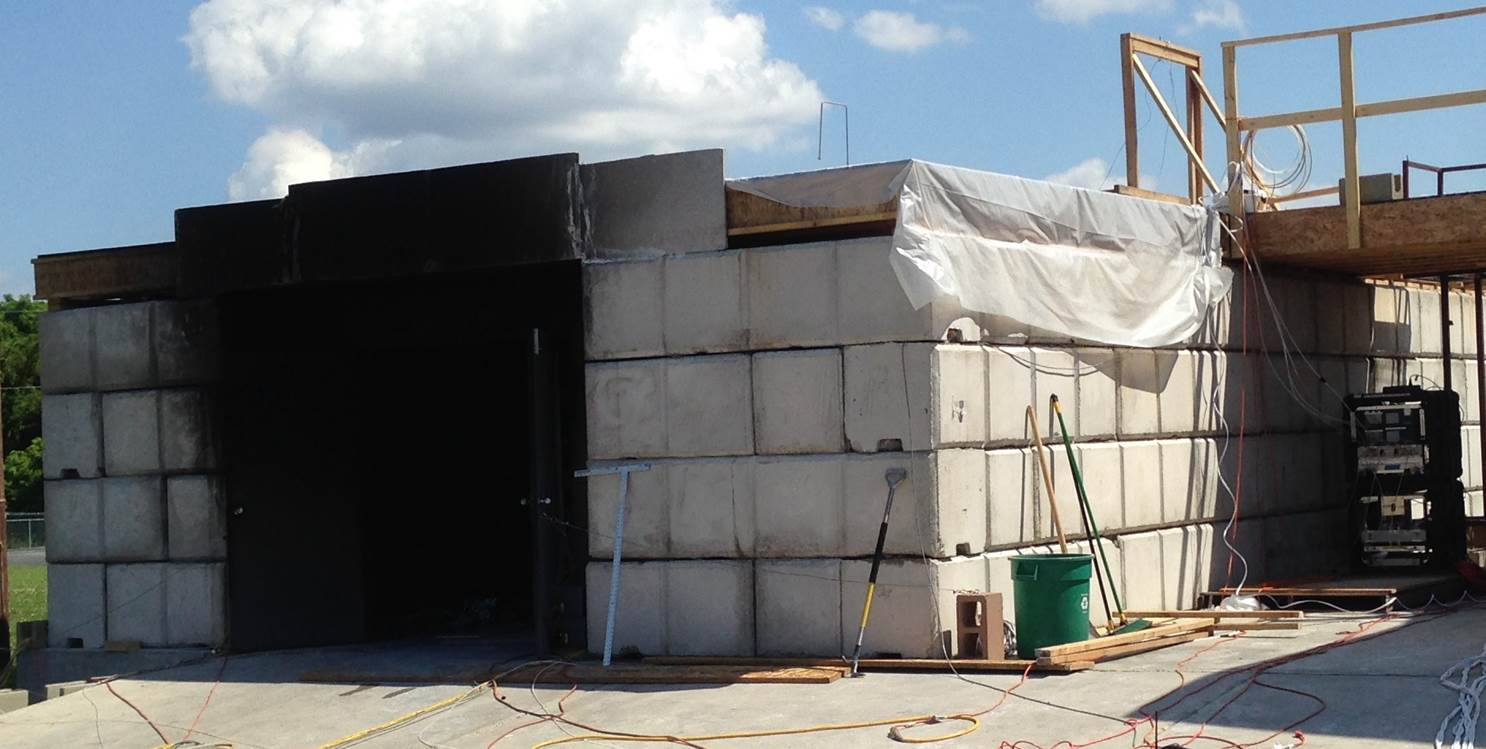
\includegraphics[width=5.25in]{../Figures/Pictures/east_structure}
	\\~\\
	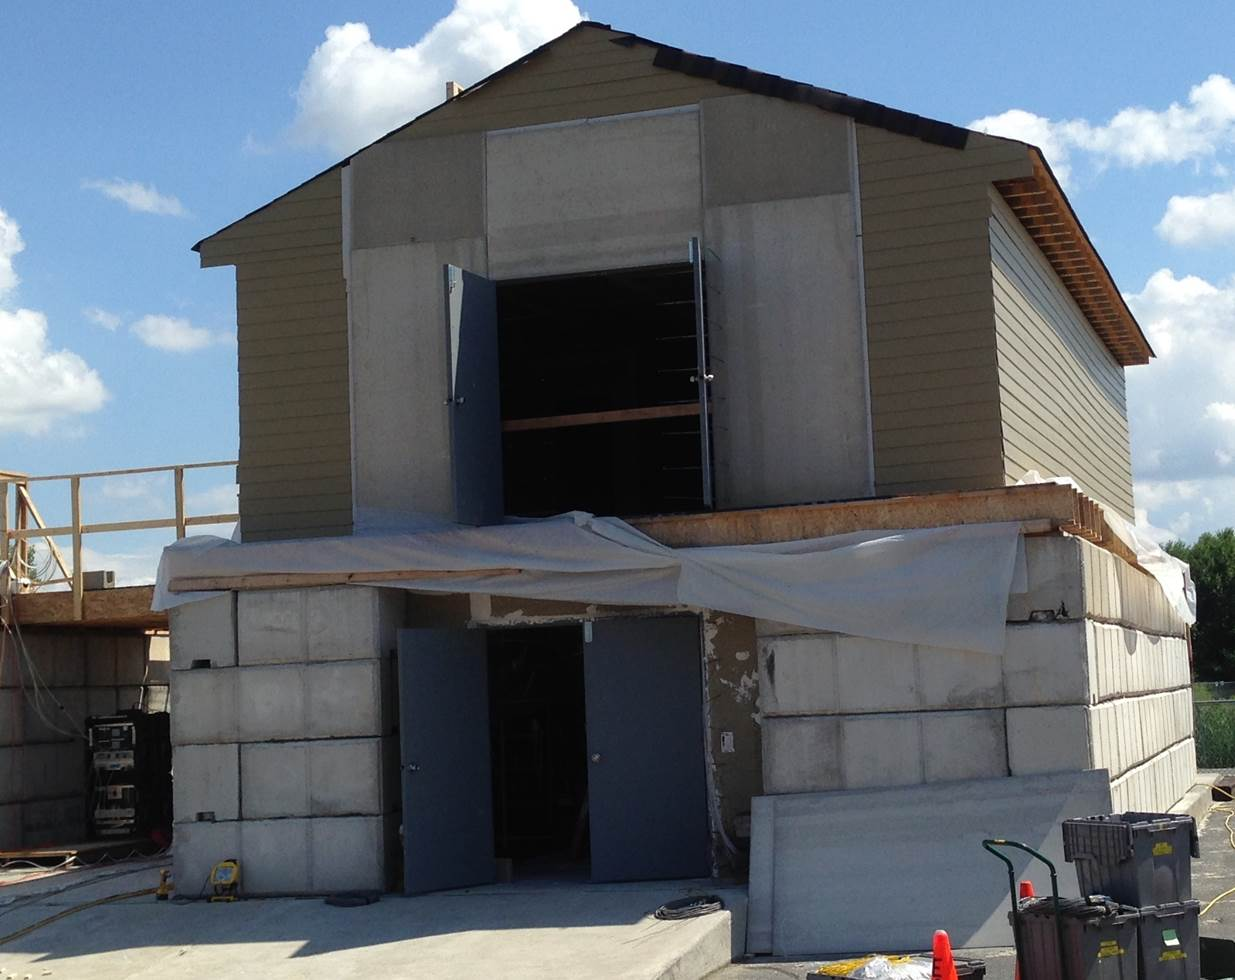
\includegraphics[width=5.25in]{../Figures/Pictures/west_structure}
	\caption[North side of the East and West Structures.]{North side of the East (top) and West (bottom) Test Structures.}
	\label{fig:struct_pics}
\end{figure}

The interior walls of the first floor of each structure were framed with steel studs set to 0.40~m (16~in) centers and track and \textit{were lined with 13~mm (0.5~in) thick cement board. The walls were composed of 16~mm (5/8~in) Type X gypsum board. Additionally, the ceiling was composed of two layers of 13~mm (0.5~in) thick cement board.}
\FloatBarrier

The first floor ceiling support of each structure was composed of wood truss joist I-beams (TJIs) with a 299~mm (11.75~in) depth. Each TJI was composed of laminated veneer lumber flanges with a cross section of 29~mm (1.13~in) x 44~mm (1.75~in) and an 11~mm (0.43~in) thick oriented strand board web as shown in Fig.~\ref{fig:TJI}. Tongue and grove, 18.3~mm (0.72~in) thick, oriented strand board was screwed to the top of the TJIs.

\begin{figure}[!ht]
	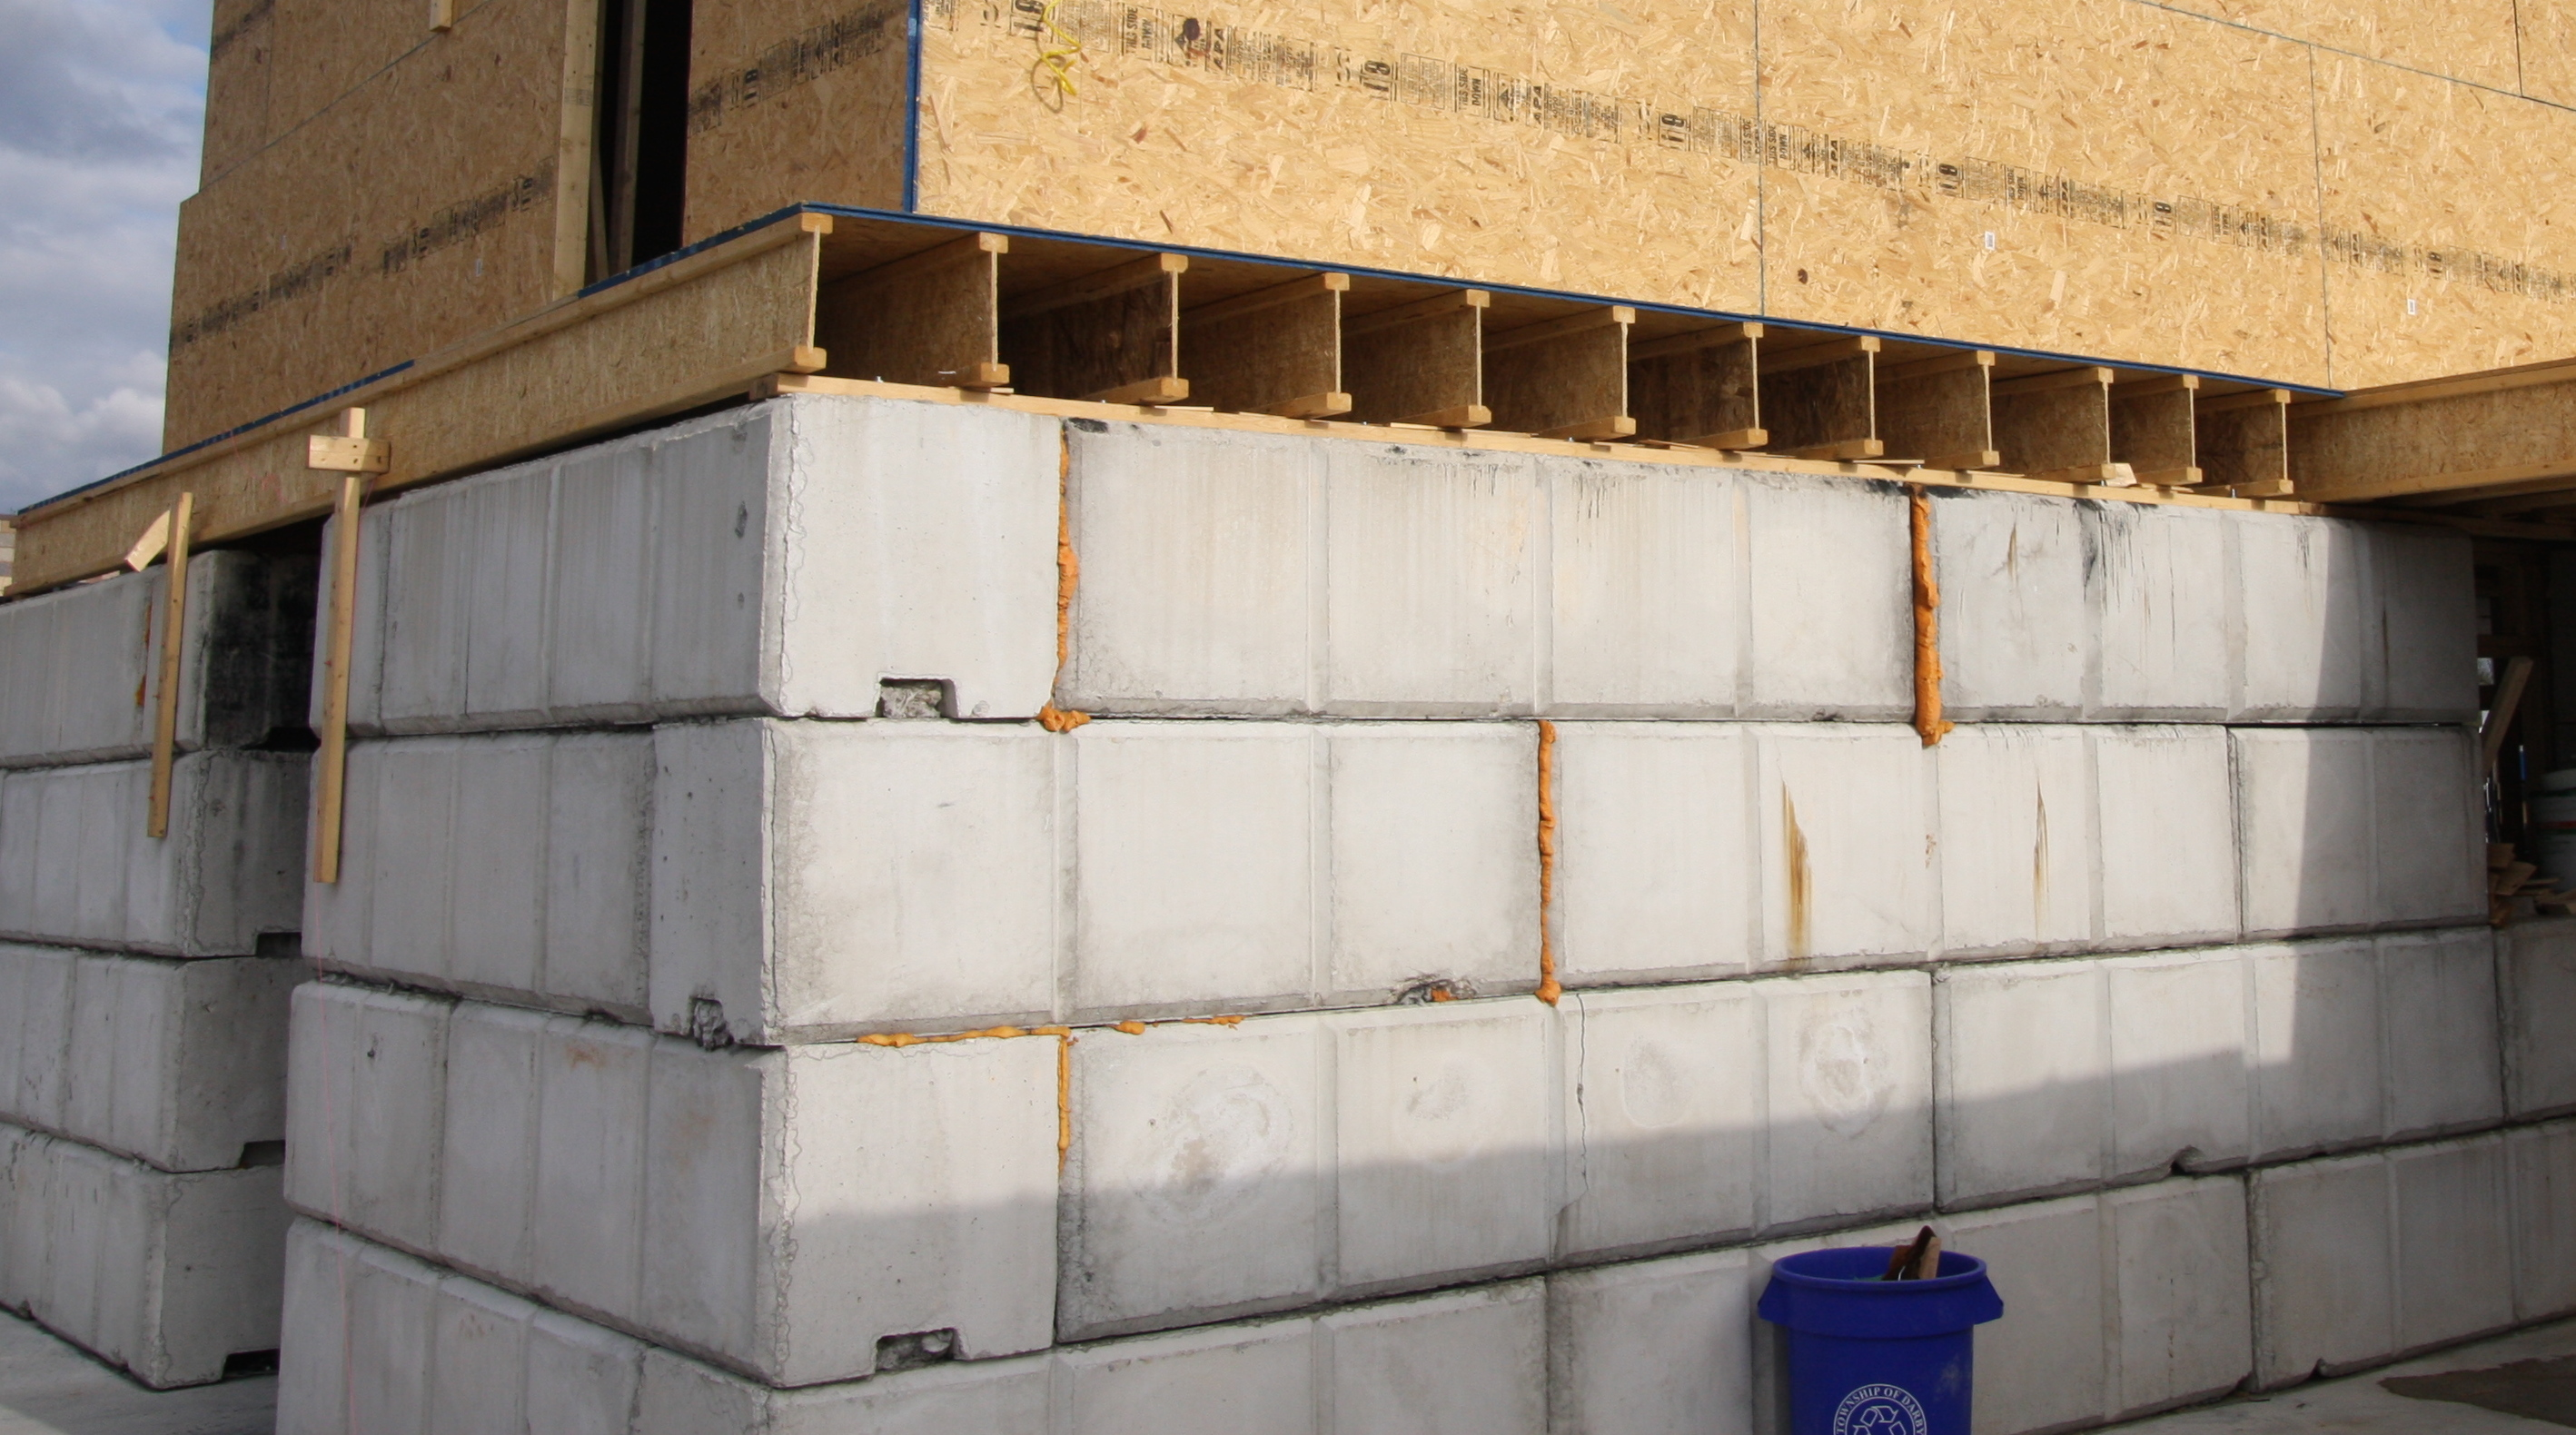
\includegraphics[width=\columnwidth]{../Figures/Pictures/TJI_support}
	\caption[TJI-constructed ceiling support of the West Structure.]{First floor ceiling support of the West Structure composed of wood truss joist I-beams. View is of the southeast corner of the structure.}
	\label{fig:TJI}
\end{figure}
\FloatBarrier

The second floor of the West Structure was built on the wood ceiling support described above and was connected to the first floor by a stairwell. The second story walls were wood framed with 51~mm (2~in) by 102~mm (4~in) studs set to 0.40~m (16~in) centers. The interior walls were protected by 16~mm (5/8~in) fire rated gypsum board, 16~mm (5/8~in) durarock board, and a second layer of 16~mm (5/8~in) fire rated gypsum board. The exterior walls were protected with 11~mm (7/16~in) oriented strand board and 8~mm (5/16~in) fiber cement lap siding.

\subsubsection{Layout}
\label{sec:layout}
Dimensioned floor plans of the East and West Structures are presented in Figures~\ref{fig:east_dimensioned_plan}~and~\ref{fig:west_dimensioned_plan}, respectively. \textbf{Add N arrow to floor plans}

\begin{figure}[!ht]
	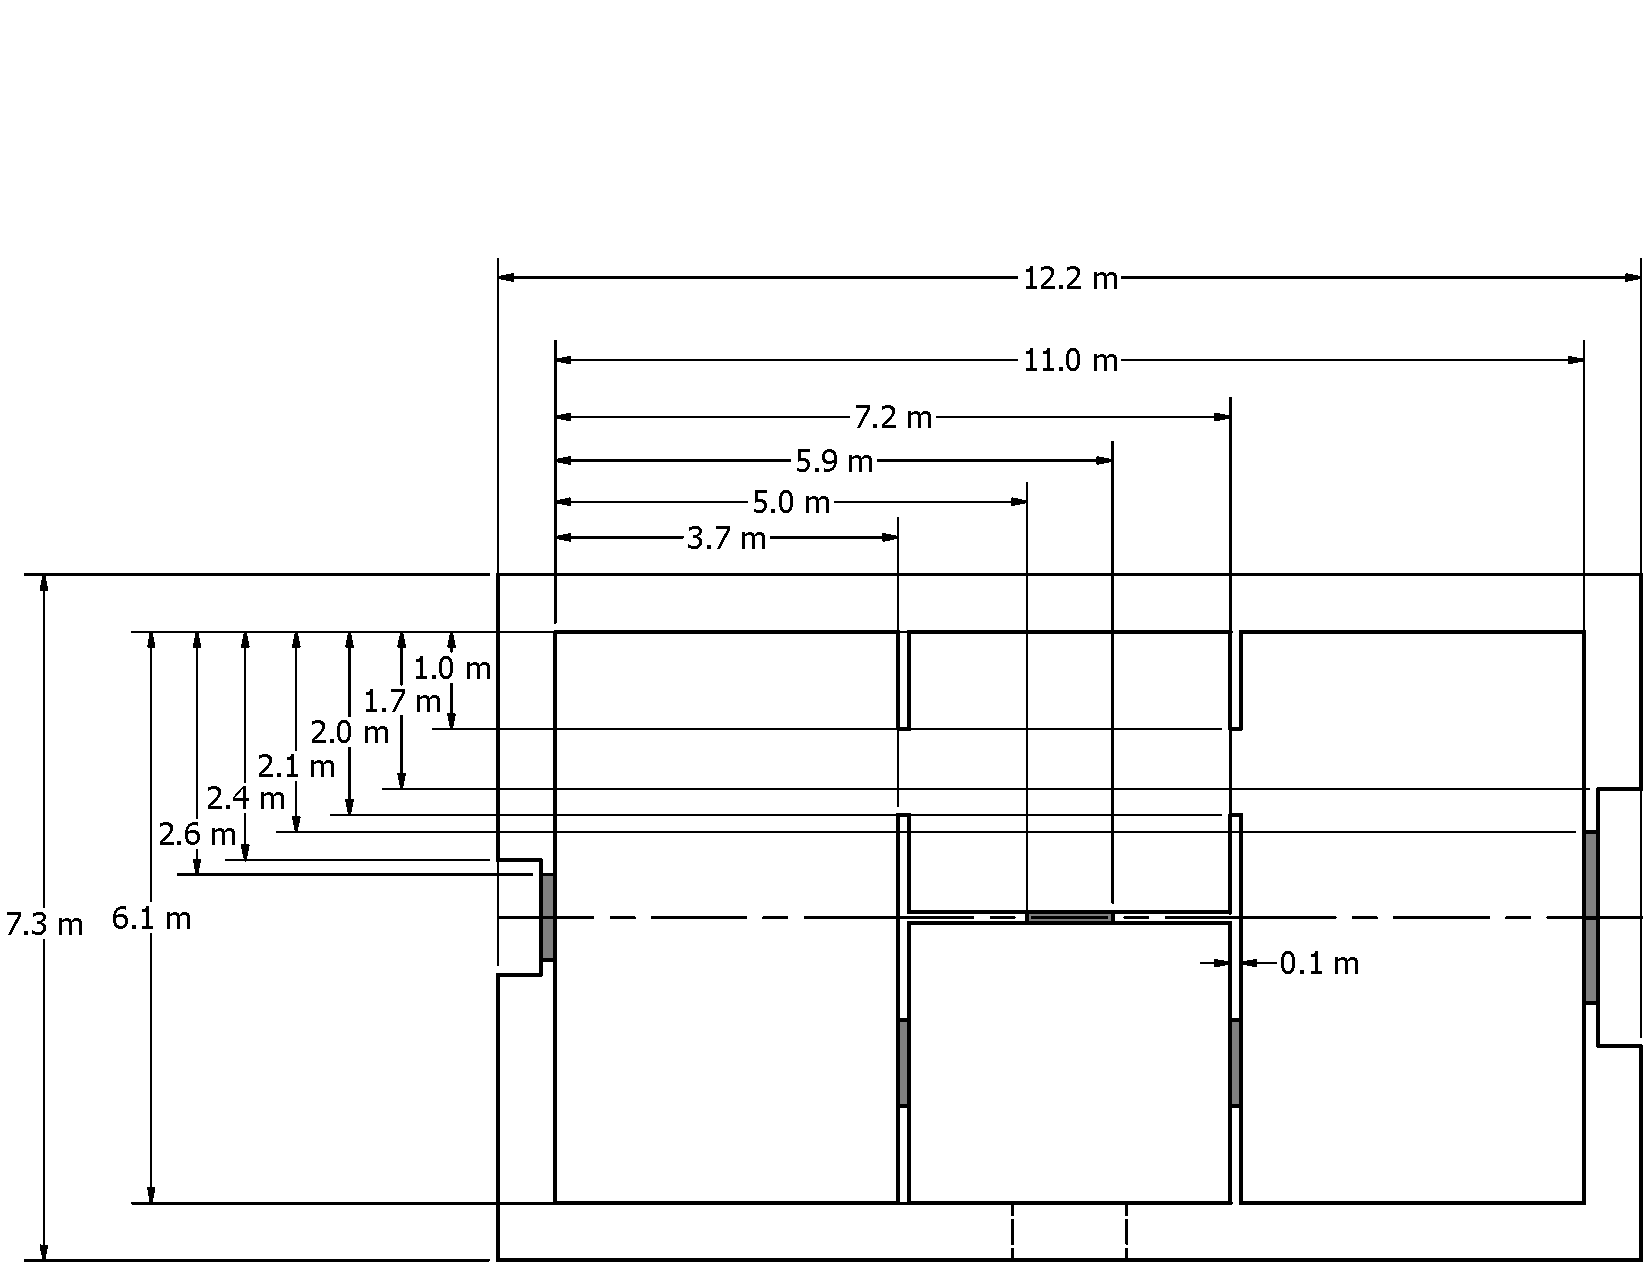
\includegraphics[width=\columnwidth]{../Figures/Floor_Plans/East_Test_Structure_Dimensioned_Full}
	\caption[Dimensioned floor plan of the East Structure.]{East Structure floor layout.}
	\label{fig:east_dimensioned_plan}
\end{figure}

\begin{figure}[!ht]
	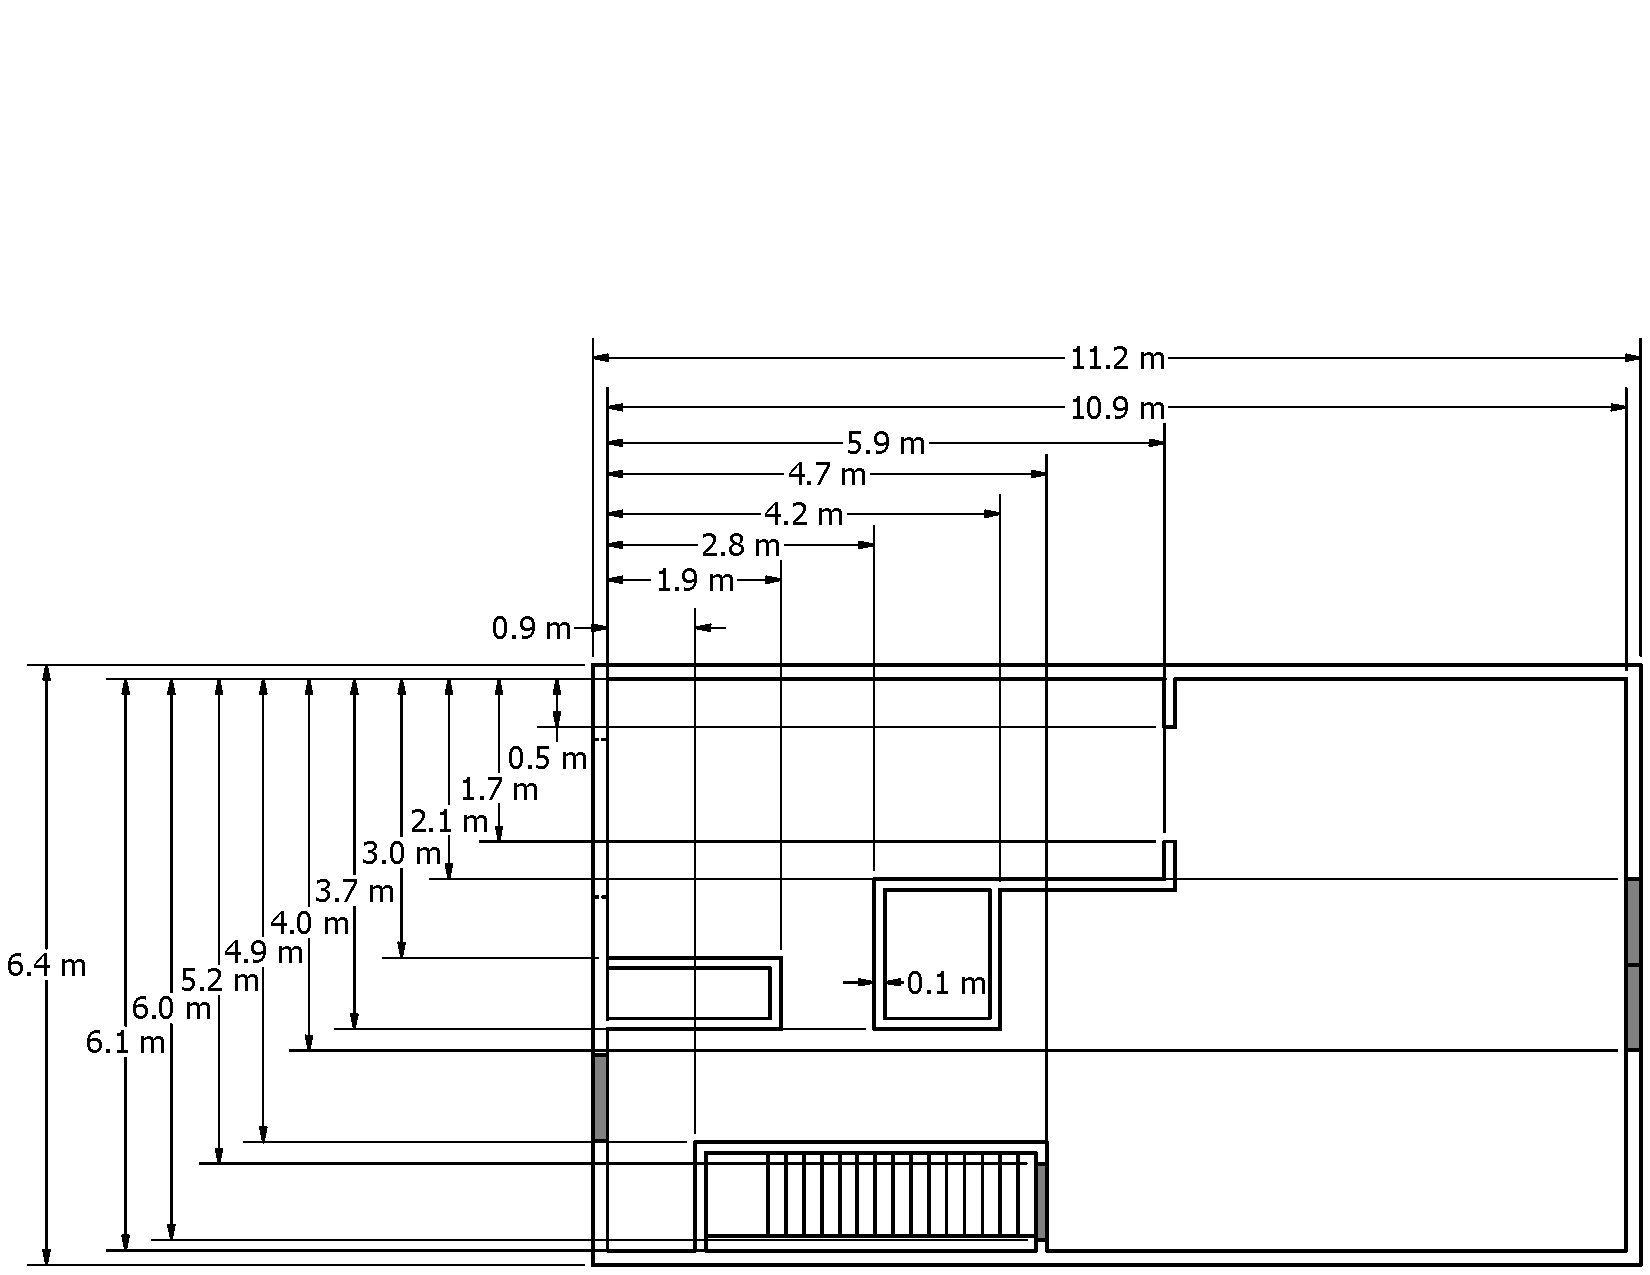
\includegraphics[width=\columnwidth]{../Figures/Floor_Plans/West_Structure_2nd_Floor_Dimensioned_Full}
	\\~\\
	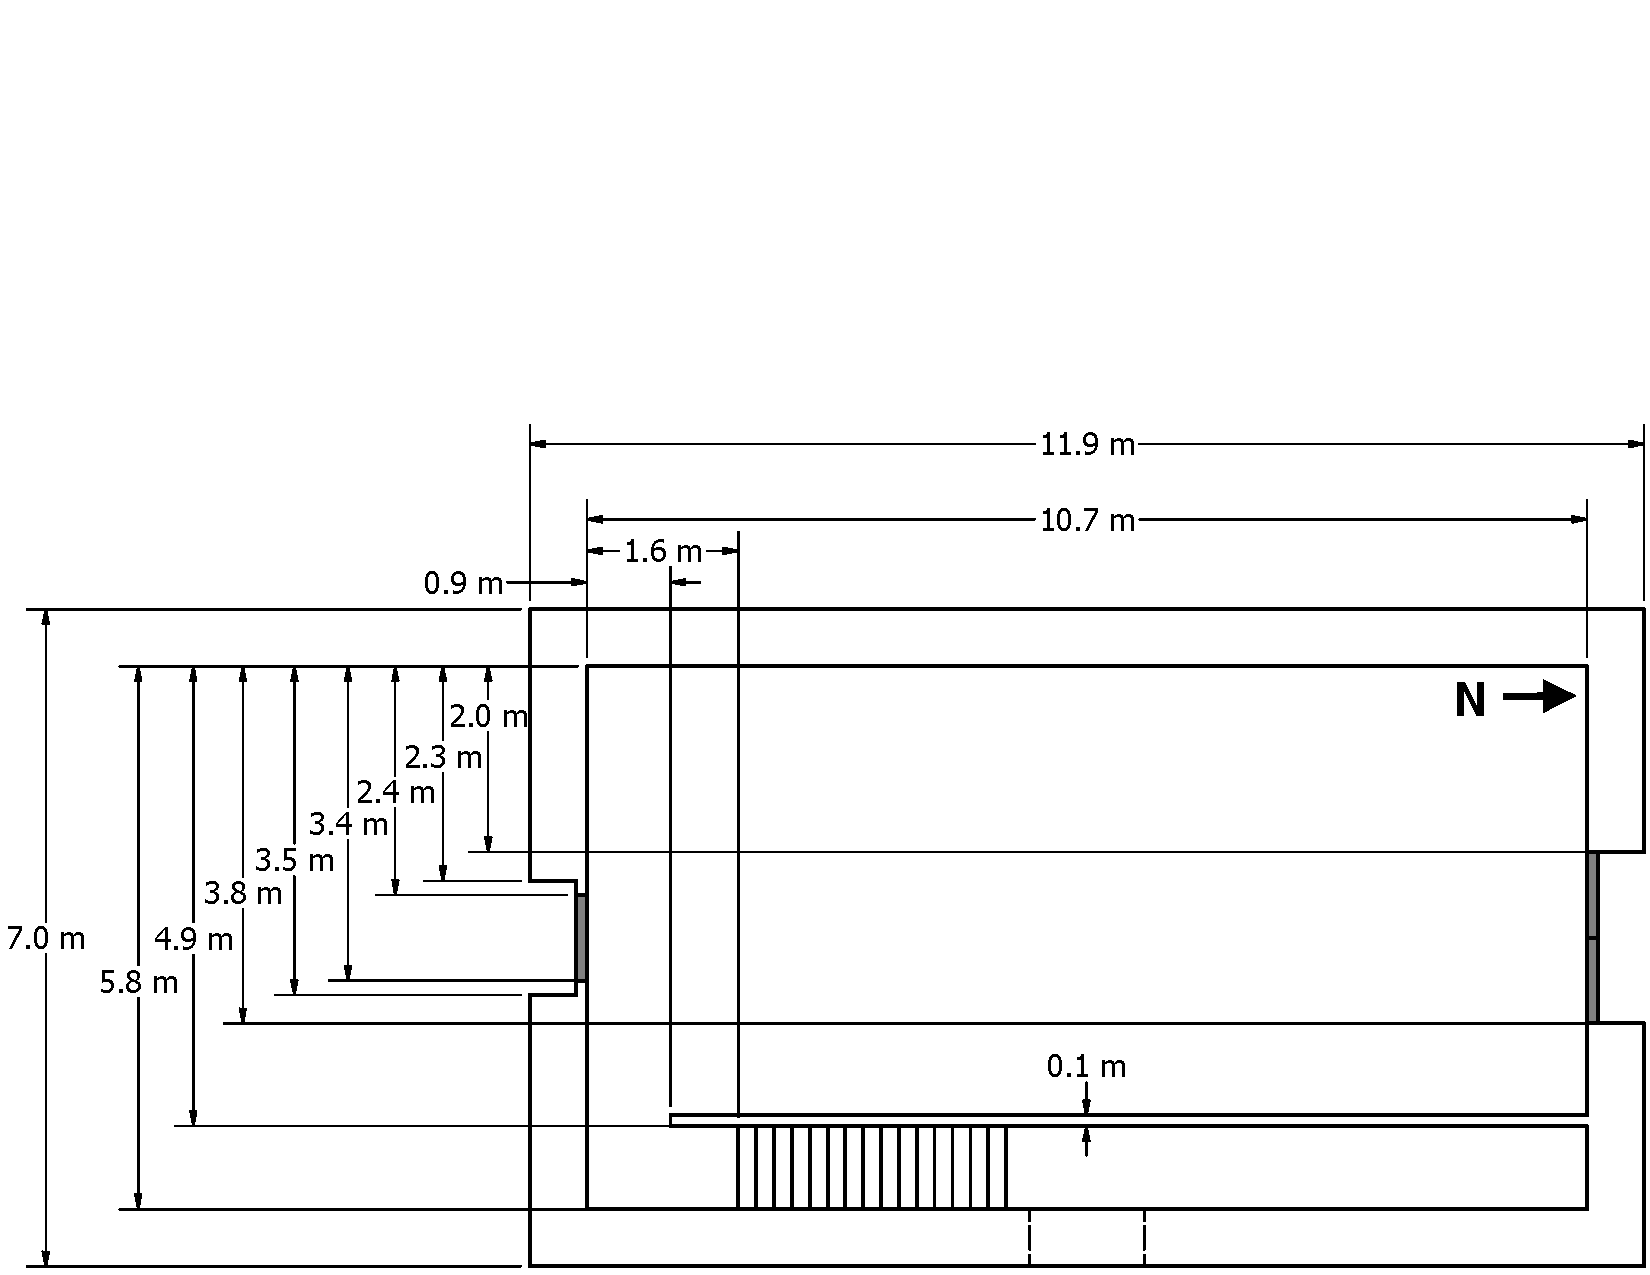
\includegraphics[width=\columnwidth]{../Figures/Floor_Plans/West_Structure_1st_Floor_Dimensioned_Full}
	\caption[Dimensioned floor plan of the first and second floors of the West Structure.]{Dimensioned floor plan of the second floor (top) and first floor (bottom) of the West Structure.}
	\label{fig:west_dimensioned_plan}
\end{figure}

The interior dimensions of each structure were approximately 6.1~m (20~ft) wide, 11~m (36~ft) long and 2.4~m (8~ft) high. The stairs connecting the two floors of the West Structure started 1.6~m (5.25~ft) off the south wall with a width of 1.2~m (4~ft) off the east wall.

The exterior doorways of each structure and the stairwell doorway on the second level of the West Structure all contained doors that were opened or closed at certain instances to change the ventilation patterns of the structure. All other doorways in the structures did not contain a door, so to close the doorway, a sheet of gypsum board was used to cover the opening and the doorway remained closed for the duration of the test procedure.
\FloatBarrier

\subsection{Instrumentation}
\label{sec:instrumentation}
A discussion of uncertainties for each type of measurement in this report can be found in Section~\ref{sec:uncertainty}. For every experiment, gas velocity at an interior doorway was measured using differential pressure transducers connected to bi-directional velocity probes~\cite{McCaffrey:Combustion_and_Flame}. An array of 6 bi-directional probes located at the northeast interior doorway of the East Structure is pictured below in Fig.~\ref{fig:BDPs}. A single thermocouple was attached to each bi-directional probes to measure the temperature to be used in conjunction with the pressure measurement to derive velocity. Every thermocouple attached to the bi-directional probes was exposed-bead, Chromel-Alumel (type K) with a 1.0~mm (0.04 in) diameter. Starting with the exposed bead, the thermocouple wire was sheathed in a 3.2~mm (0.13 in) diameter Inconel shield that was 0.76~m (2.5~ft) in length. 

The approximate locations of the bi-directional probes used to measure air velocity are annotated in the plan views of the East Structure and West Structure experimental setups (Fig.~\ref{fig:east_setup} and Figs.~\ref{fig:flow_path_1}-\ref{fig:flow_path_2}, respectively) found in Section~\ref{sec:exp_procedure}. To minimize potential measurement errors due to external environmental conditions (i.e., wind), only velocity data measured by bi-directional probes located at interior doorways are considered in this report. The set of bi-directional probes at the northeast interior doorway of the East Structure, denoted as ``A6", contained 6 probes located at distances of 0.30 m, 0.60 m, 0.90 m, 1.20 m, 1.50 m, and 1.80~m below the soffit of the doorway. The set of bi-directional probes at the interior doorway in the West Structure, denoted as ``A10", contained 8 probes located at distances of 0.08 m, 0.34 m, 0.61 m, 0.88 m, 1.15 m, 1.42 m, 1.68 m, and 1.95~m below the soffit of the corresponding doorway.

\begin{figure}[!ht]
	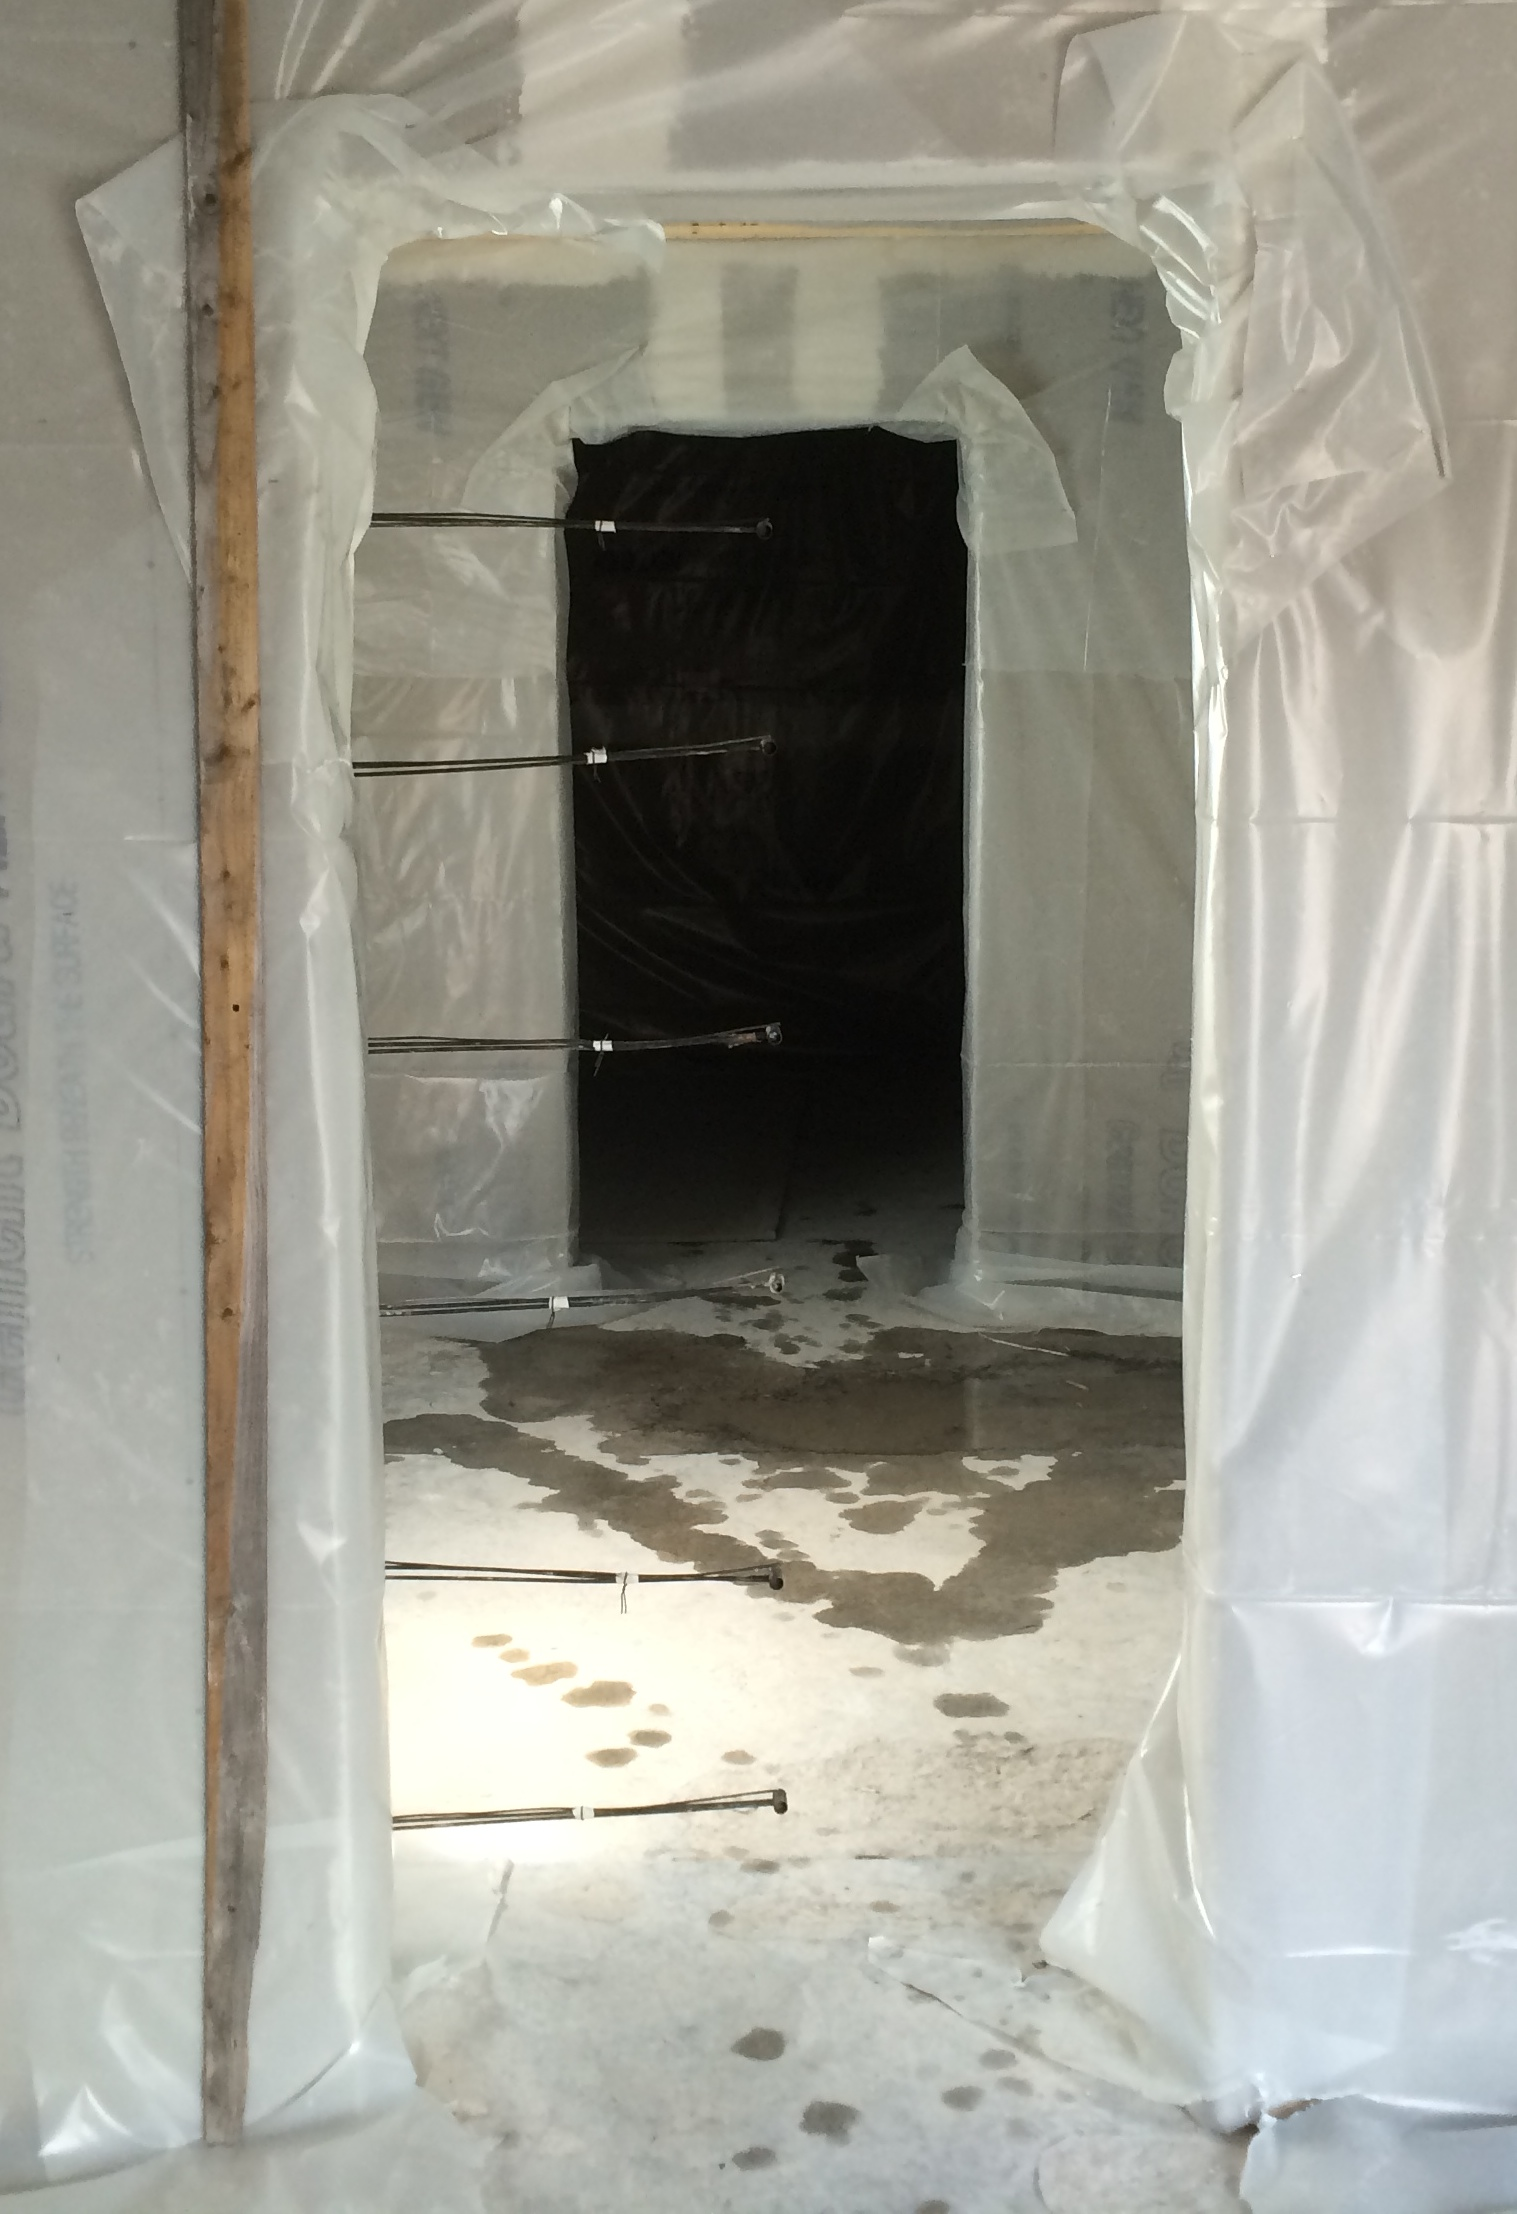
\includegraphics[width=3.5in]{../Figures/Pictures/BDPs_east}
	\caption[Array of bi-directional probes at interior doorway in East Structure.]{Array of bi-directional probes located at the northeast interior doorway in the East Structure. View is looking at the array from Room C.}
	\label{fig:BDPs}
\end{figure}
\FloatBarrier

\subsection{Uncertainty}
\label{sec:uncertainty}
There are different components of uncertainty in the length, differential pressure, flow rate, and gas velocity reported here. Uncertainties are grouped into two categories according to the method used to estimate them. Type A uncertainties are those which are evaluated by statistical methods, and Type B are those which are evaluated by other means~\cite{Taylor&Kuyatt:1994}. Type B analysis of systematic uncertainties involves estimating the upper (+a) and lower (-a) limits for the quantity in question such that the probability that the value would be in the interval ($\pm$a) is essentially 100\%. After estimating uncertainties by either Type A or B analysis, the uncertainties are combined in quadrature to yield the combined standard uncertainty. Then, the combined standard uncertainty is multiplied by a coverage factor of two, which results in the expanded uncertainty with a 95\% confidence interval (2$\sigma$). For some of these components, such as the zero and calibration elements, uncertainties are derived from referenced instrument specifications. For other components, referenced research results and past experience with the instruments provided input in the uncertainty determination. 

Each length measurement was taken carefully. Length measurements such as the room dimensions, instrumentation array locations, and fire apparatus (e.g., nozzle, sprinkler, or fan) placement were made with a hand held laser measurement device which has an accuracy of $\pm$6.0~mm (0.25~in) over a range of 0.61~m (2.0~ft) to 15.3~m (50.0~ft)~\cite{StanleyTools}.  However, conditions affecting the measurement, such as levelness of the device, yields an estimated uncertainty of $\pm$0.5\% for measurements in the 2.0~m (6.6~ft) to 10.0~m (32.8~ft) range. Steel measuring tapes with a resolution of $\pm$0.5~mm (0.02~in) were used to locate individual sensors within a measurement array and to measure and position the furniture. The steel measuring tapes were manufactured in compliance with NIST Manual 44, which specifies a tolerance of $\pm$1.6~mm (0.06~in) for 9.1~m (30~ft) tapes and $\pm$6.4~mm (0.25~in) for 30.5~m (100~ft) tapes~\cite{Butcher:2012}. Some issues, such as ``soft'' edges on the upholstered furniture, result in an estimated total expanded uncertainty of $\pm$1.0\%.

Bi-directional probes with pressure transducers and single thermocouples were used to measure the gas velocity. Bare-bead Type K thermocouples were co-located with the probe. A gas velocity measurement study, examining the doorway flow of pre-flashover compartment fires, yielded expanded uncertainty measurements ranging from $\pm0.14$ to $\pm0.22$ for bi-directional probes of similar design~\cite{Bryant:FSJ2009}. The total expanded uncertainty for gas velocity in these experiments is estimated to be $\pm18$\%.   

Water flow rate was measured with a pressure and flow meter combination shown in Fig.~\ref{fig:flow_meter}. The meter consists of a section of 6.35 cm (2.5 in) cast aluminum pipe with a 0-4.1 MPa (0-600 psi) pressure transducer and a paddlewheel type flow sensor with a range of 0 to 4800 lpm (1250 gpm). The pressure transducer and paddlewheel both connect to the battery operated control box where the pressure transducer voltage is converted to a pressure and the paddlewheel pulse count is converted to a volumetric flow rate. The manufacturer reports a $\pm5$\% calibration expanded uncertainty for the flow sensor and $\pm3$\%  for the pressure sensor~\cite{Akron}. The pressure transducer was calibrated with a known analog pressure gauge. The flow meter was calibrated by capturing water over time and measuring that mass of water to determine the flow rate. The total expanded uncertainty was estimated at $\pm10$\%. 

\begin{figure}[!ht]
	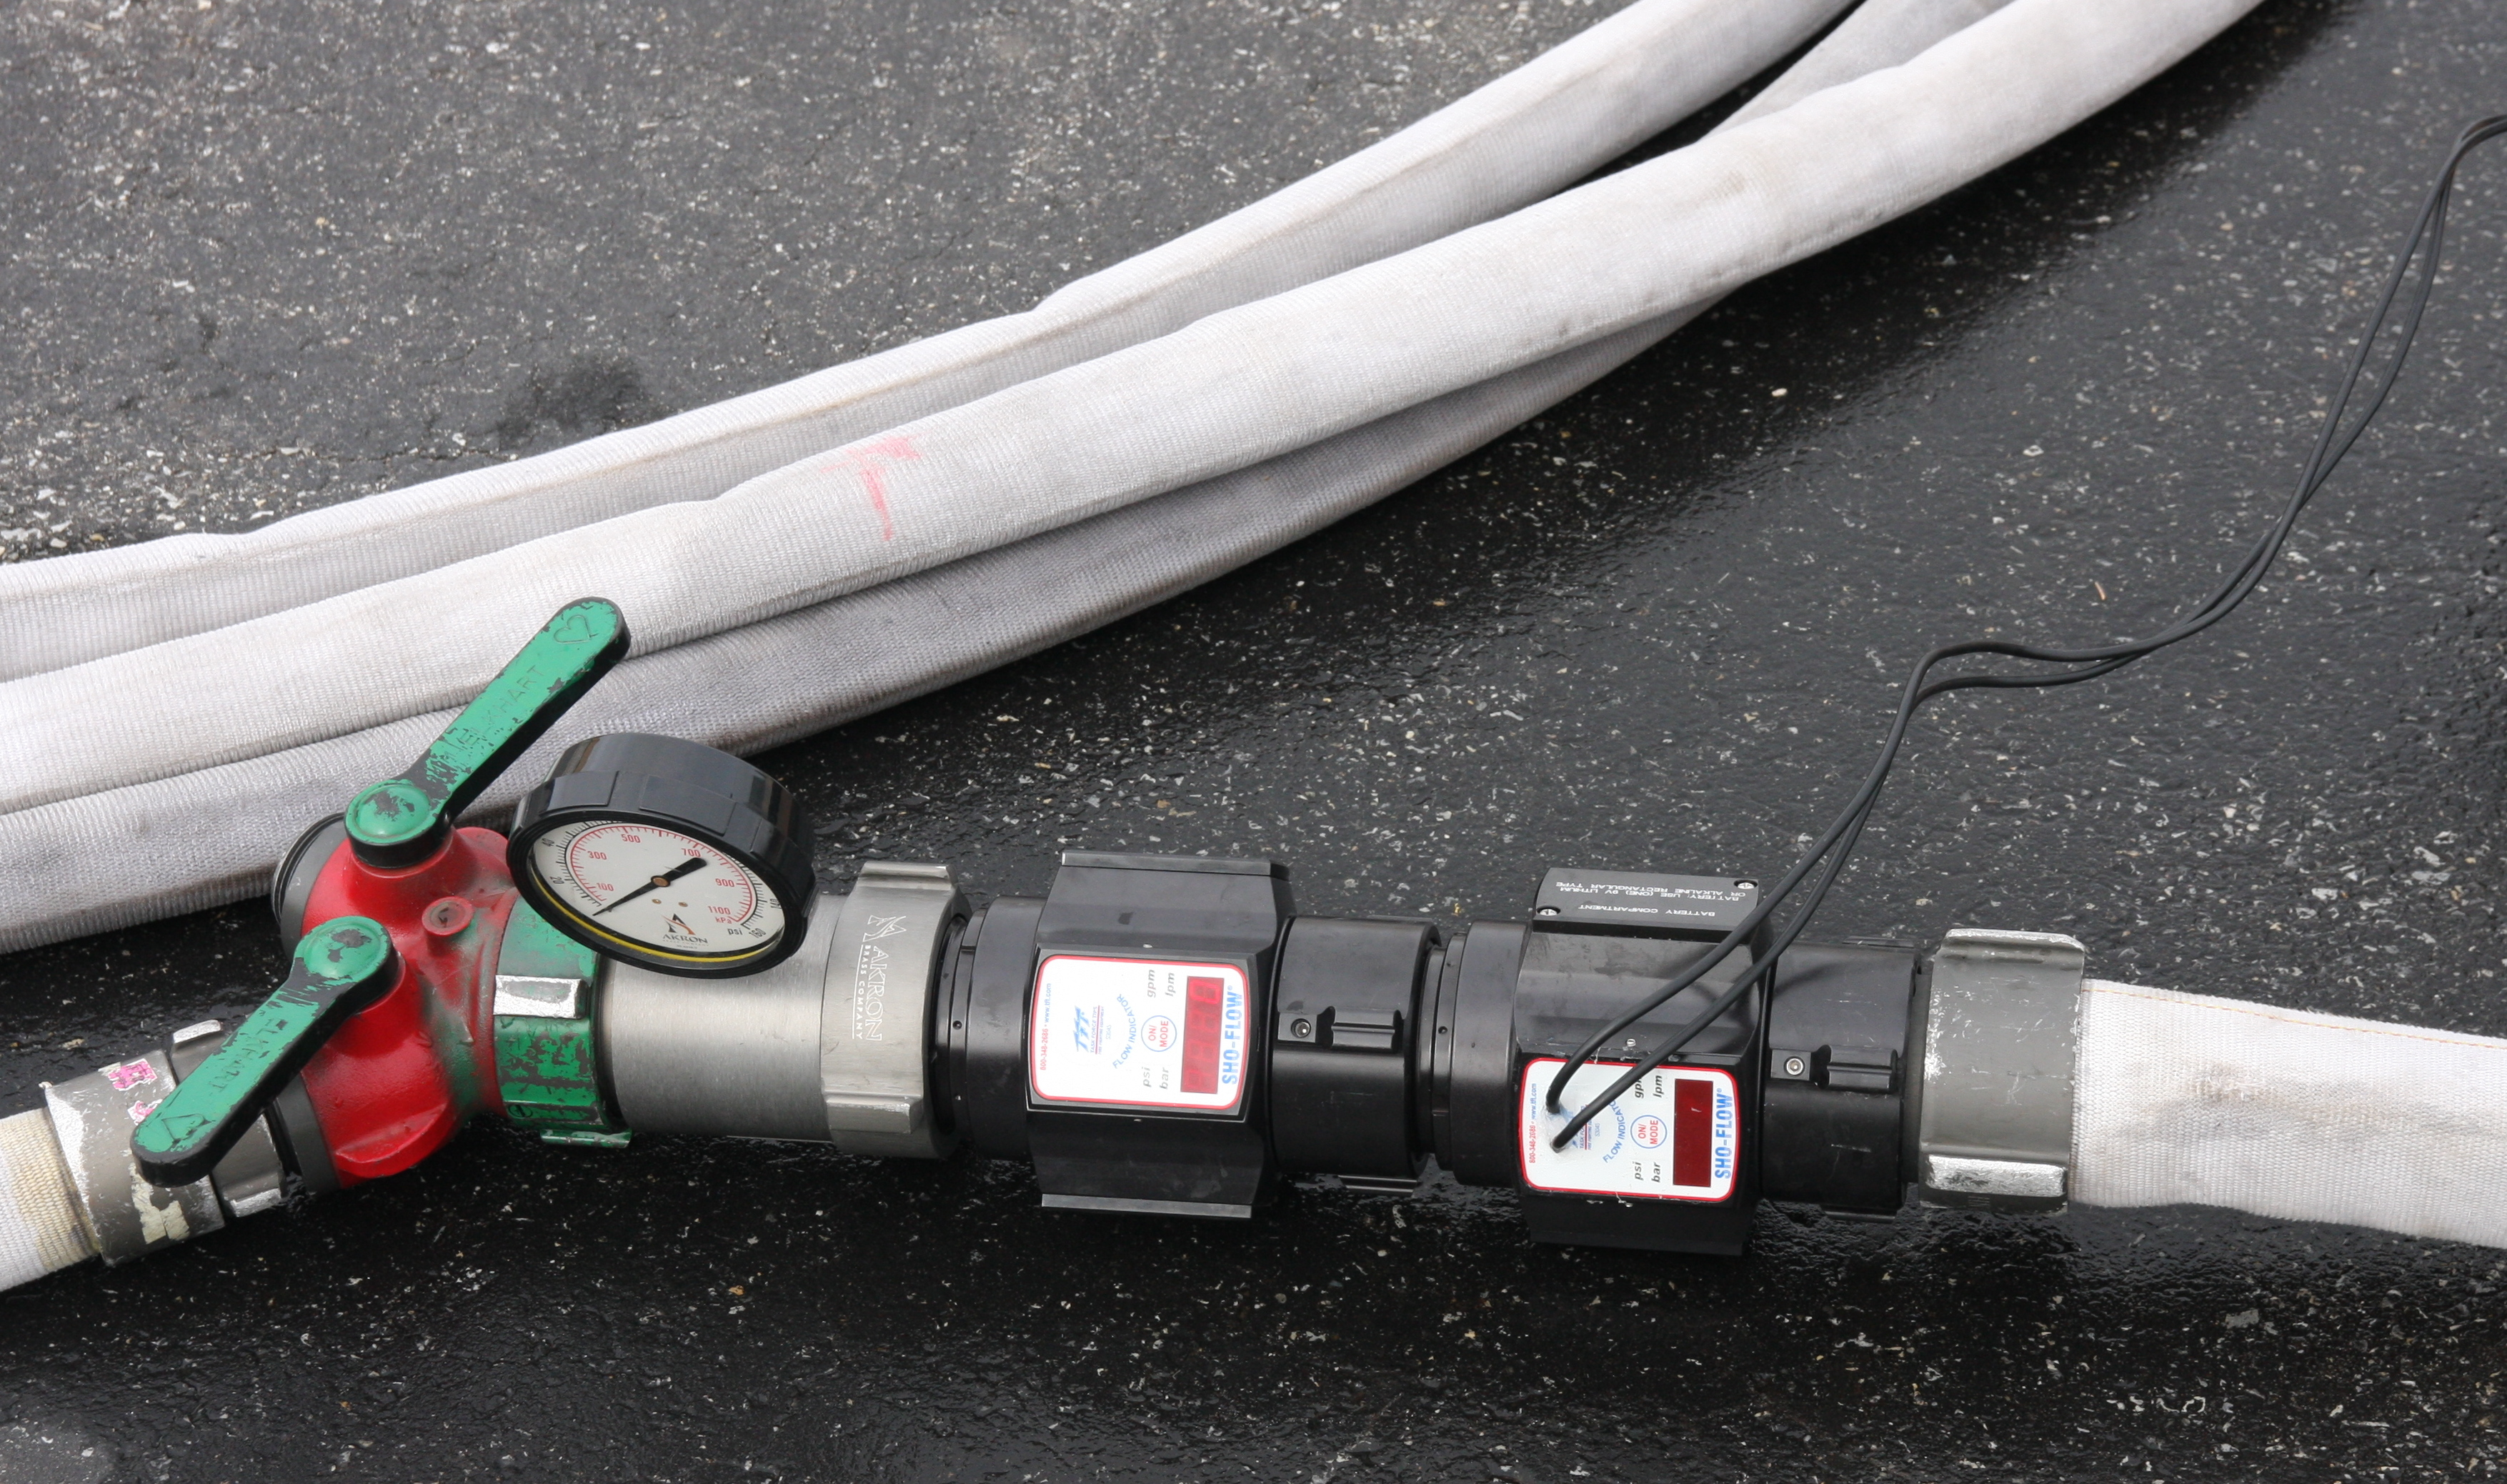
\includegraphics[width=4in]{../Figures/Pictures/flow_meter}
	\caption[Flow meter used to measure flow rate during experiments.]{Pressure and flow meter combination used to measure water flow rate during the experiments.}
	\label{fig:flow_meter}
\end{figure}
\FloatBarrier

\section{Experimental Procedure}
\label{sec:exp_procedure}
Every experiment discussed in this report involved discharging water at a known flow rate from a combination nozzle set to flow water in a straight, narrow fog, or wide fog stream pattern or from a smooth bore nozzle in a solid stream pattern. Specific doors were opened or closed before and/or during the experiments to change the ventilation in the structure. 

A total of seven test series were conducted to study the impact of different hose stream and application patterns on gas movement in a structure; three used a combination nozzle attached to a monitor to flow water at 120~GPM, three used a combination nozzle attached directly to a hoseline to flow water at 120~GPM (Fig.~\ref{fig:monitor+handline}), and one used combination and smooth bore nozzles attached to a monitor to flow water at 180~GPM. Experiments that used a monitor to flow water always applied the stream in a fixed position and thus were focused on changing the location of water application in addition to the stream pattern, while the experiments that used a combination nozzle attached directly to a hoseline to flow water focused on varying the pattern in which water was applied in addition to the stream pattern.

\begin{figure}[!ht]
	\minipage{3in}
	\begin{center}
		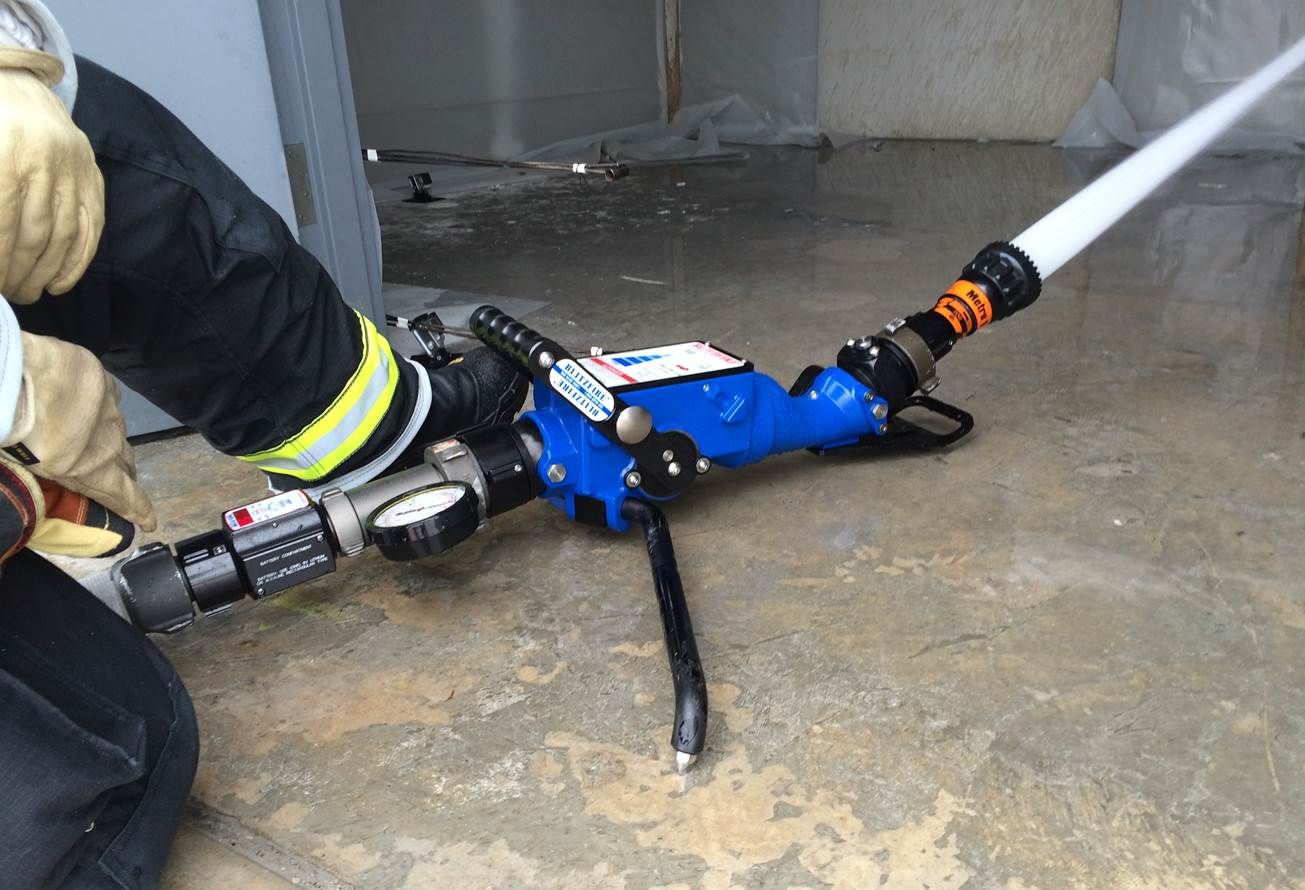
\includegraphics[width=2.9in]{../Figures/Pictures/monitor}
	\end{center} 
	\endminipage \hfill
	\minipage{3in}
	\begin{center}
		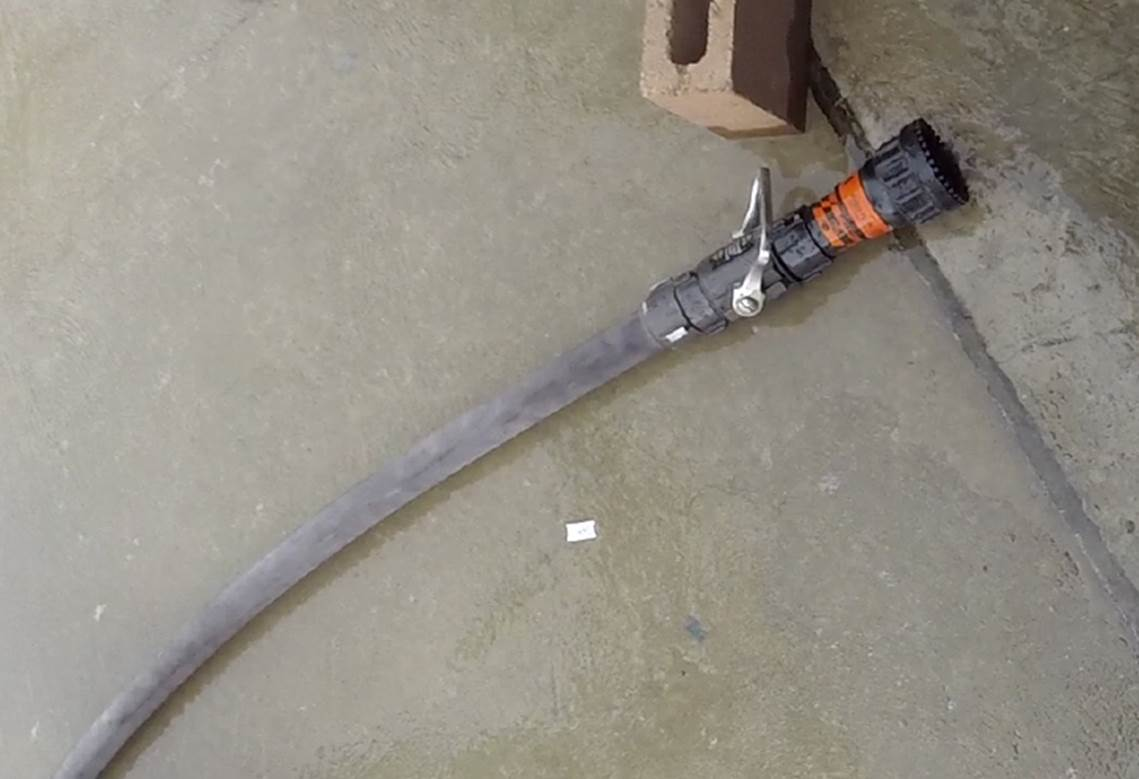
\includegraphics[width=2.9in]{../Figures/Pictures/handline}
	\end{center}
	\endminipage \hfill
	\caption[Monitor and handline equipped with a combination nozzle.]{Monitor (left) and 1.75~in handline (right) equipped with a combination nozzle and used to flow water during experiments.}
	\label{fig:monitor+handline}
\end{figure}
\FloatBarrier

Three different layouts were used for the seven test series. The test series conducted in the East Structure, Tests 33 and 34, were performed using an identical structure layout, presented in Fig.~\ref{fig:east_setup}. Test 33 used a monitor and combination nozzle to flow water and Test 34 used a combination nozzle attached directly to a handline to flow water.

The main difference between the two layouts used for the West Structure experiments is the position of the south side door on the first level. Tests 16 and 18 used the configuration with the door opened (Fig.~\ref{fig:flow_path_1}) and Tests 17, 19, and 70 used the configuration with the door closed (Fig.~\ref{fig:flow_path_2}). Tests 16 and 17 used a combination nozzle attached to a monitor to flow water; Tests 18 and 19 used a combination nozzle attached directly to a handline to flow water; and Test 70 used a combination nozzle and a smooth bore nozzle attached to a monitor to flow water in a straight and solid stream, respectively. 

\begin{figure}[!ht]
	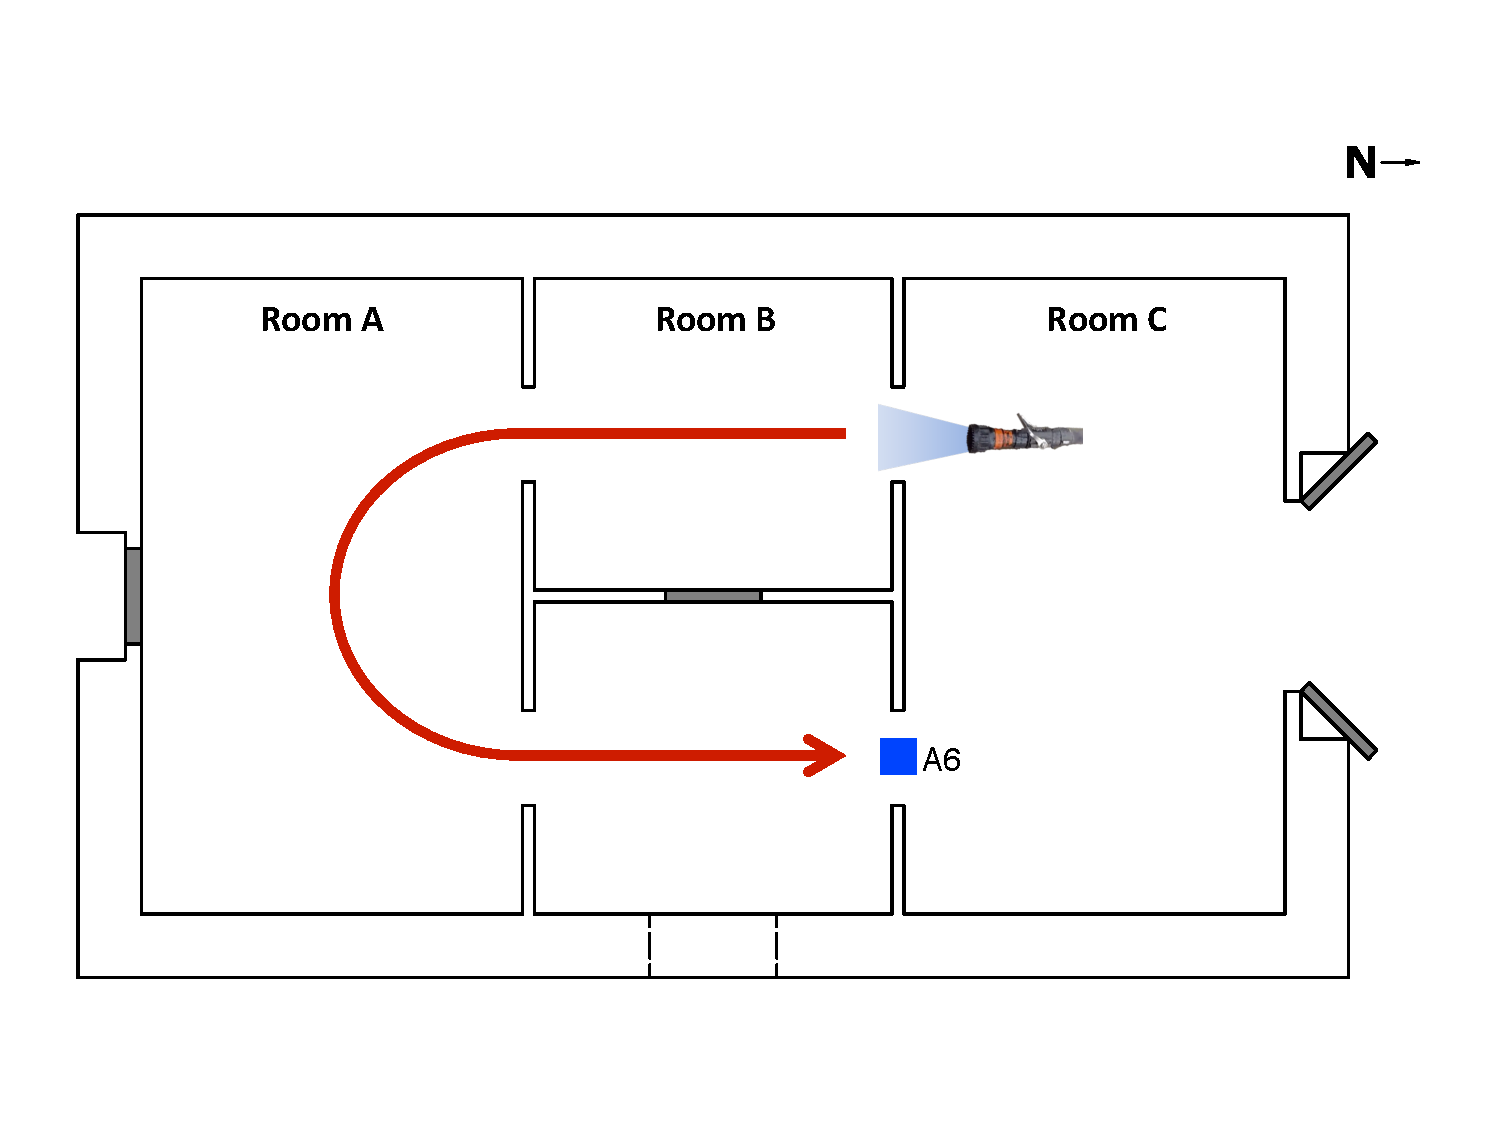
\includegraphics[width=\columnwidth]{../Figures/Floor_Plans/Specific_Tests/East_Hose_Test_Annotated}
	\caption[Plan view of the East Structure setup for Tests 33 and 34.]{Plan view of the East Structure setup for Tests 33 and 34. The view is annotated with the approximate location of water flow (nozzle graphic), the direction of the established flow path (red line), and the approximate location of A6 (blue square).}
	\label{fig:east_setup}
\end{figure}

\begin{figure}[!ht]
	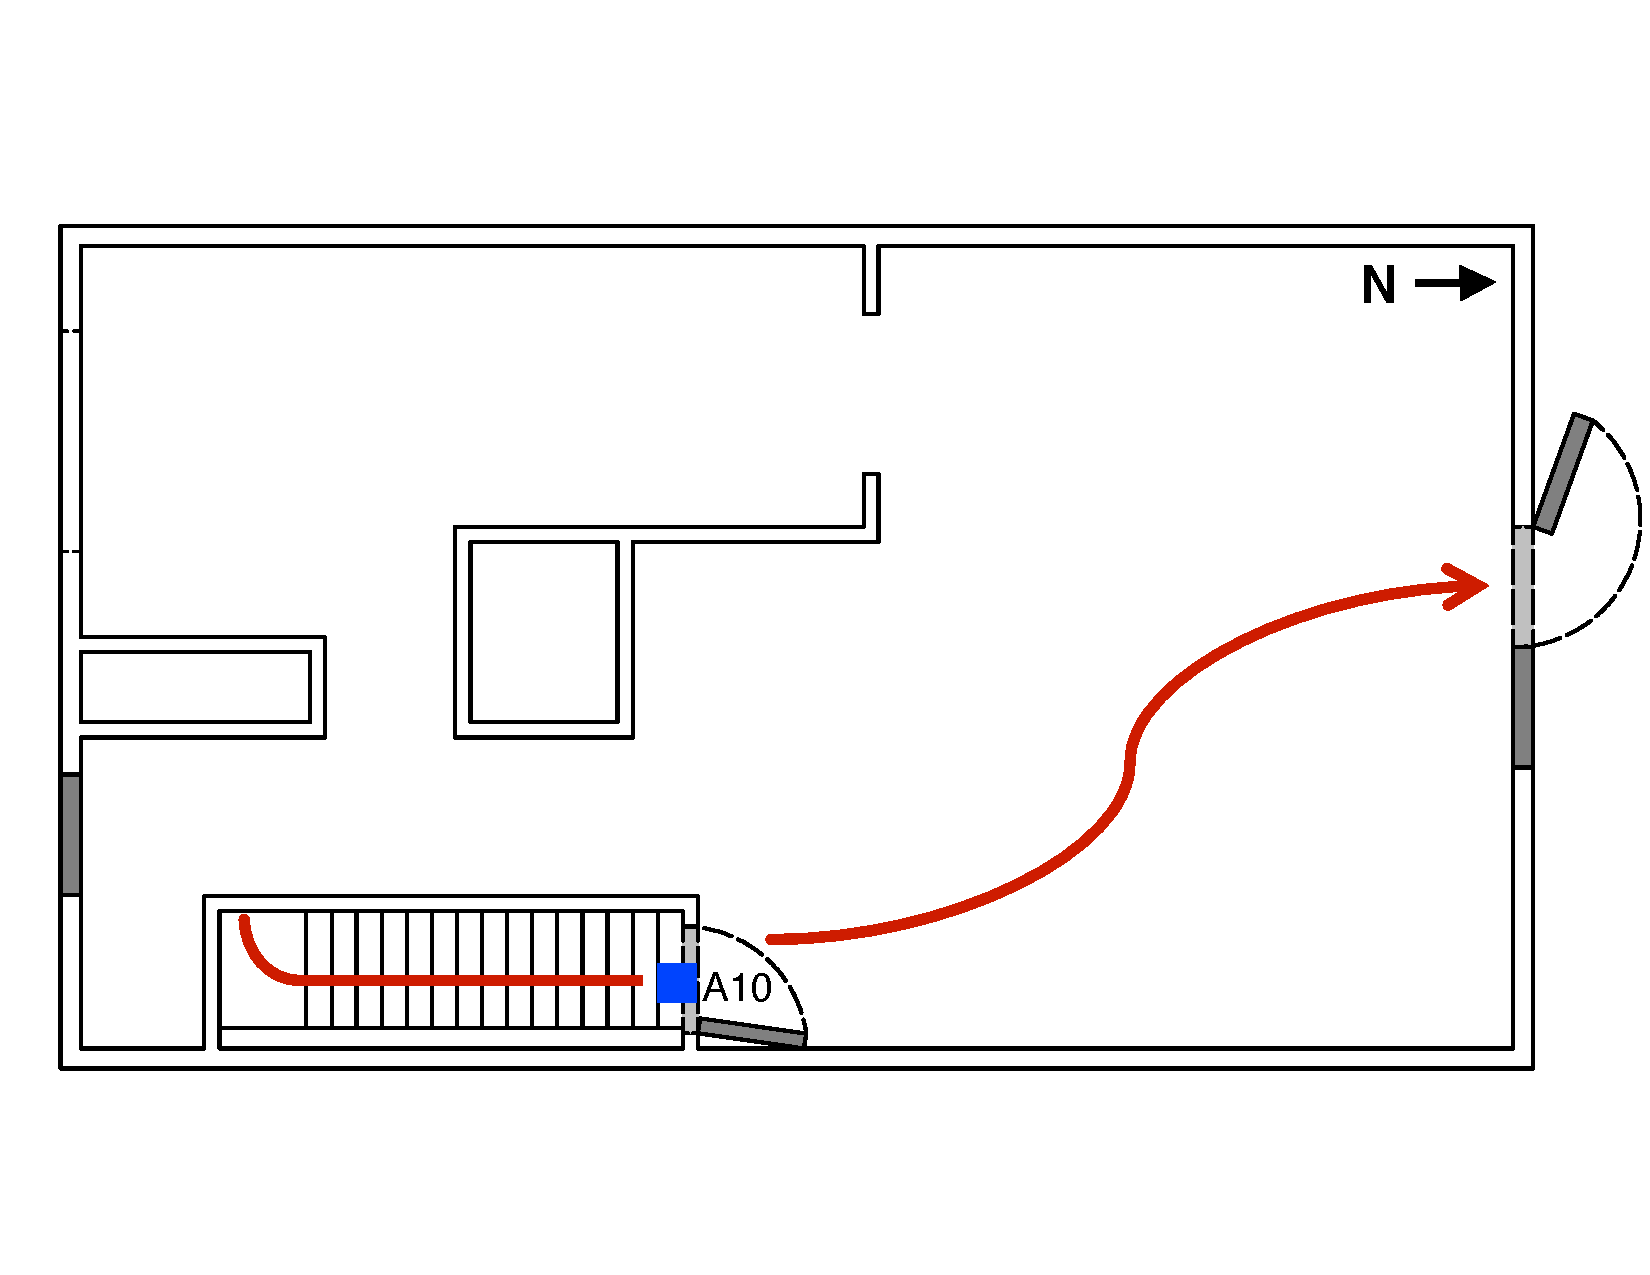
\includegraphics[width=\columnwidth]{../Figures/Floor_Plans/Specific_Tests/West_Hose_Test_2nd_Floor_Annotated}
	\\~\\
	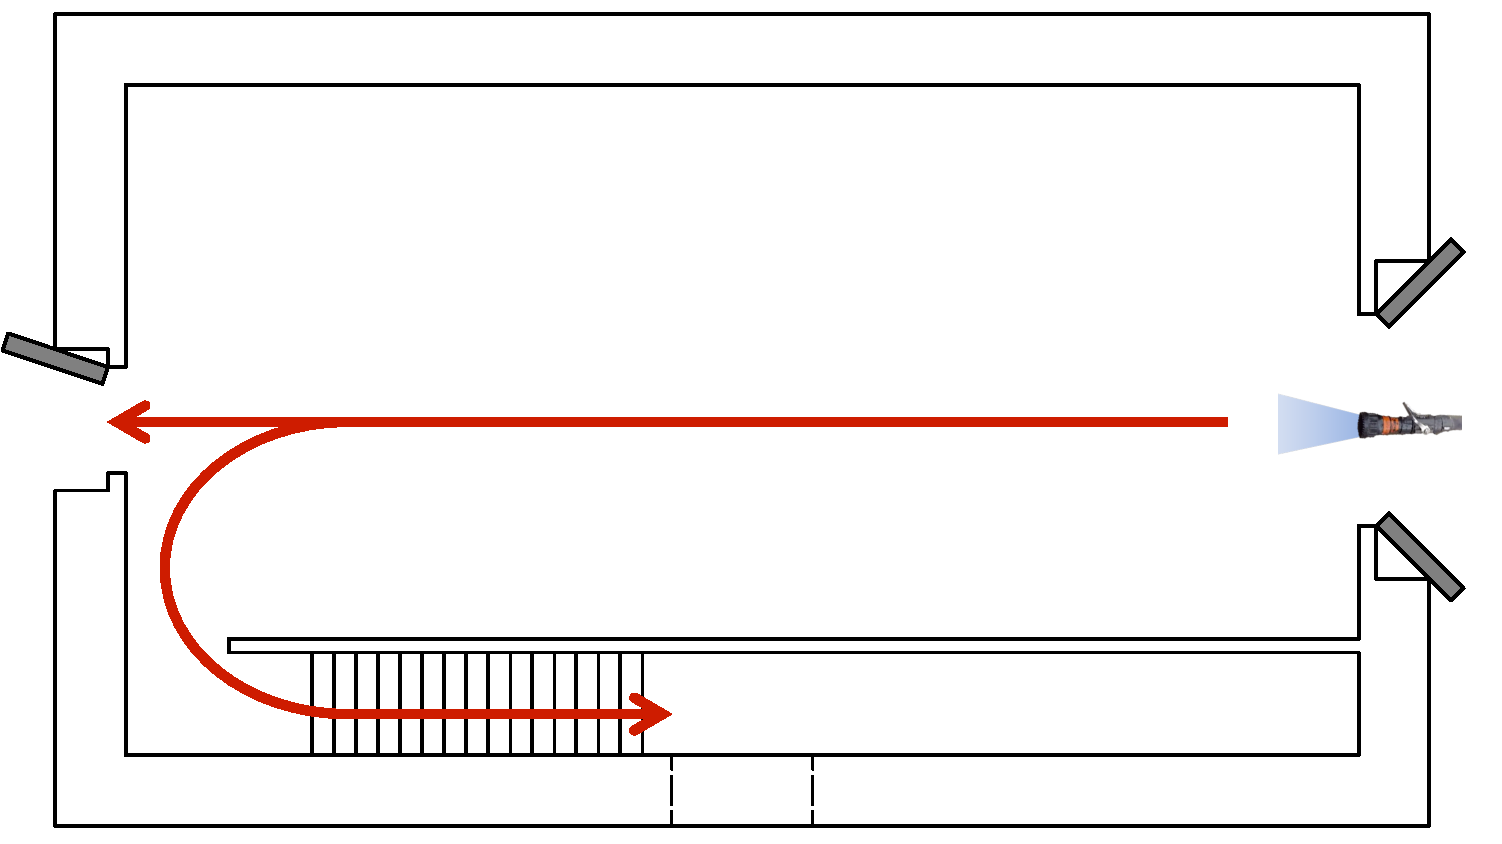
\includegraphics[width=\columnwidth]{../Figures/Floor_Plans/Specific_Tests/West_Hose_Test_18_1st_Floor_Annotated}
	\caption[Plan view of the West Structure setup for Tests 16 and 18.]{Plan view of the second floor (top) and first floor (bottom) setup in the West Structure for Tests 16 and 18. The approximate location of water flow (nozzle graphic), the direction of the established flow path (red line), and the approximate location of A10 (blue square). On the second floor, the stairwell door and north side, west double door were opened and closed at certain instances during the tests; the flow path was considered fully established when both doors were in the opened position.}
	\label{fig:flow_path_1}
\end{figure}

\begin{figure}[!ht]
	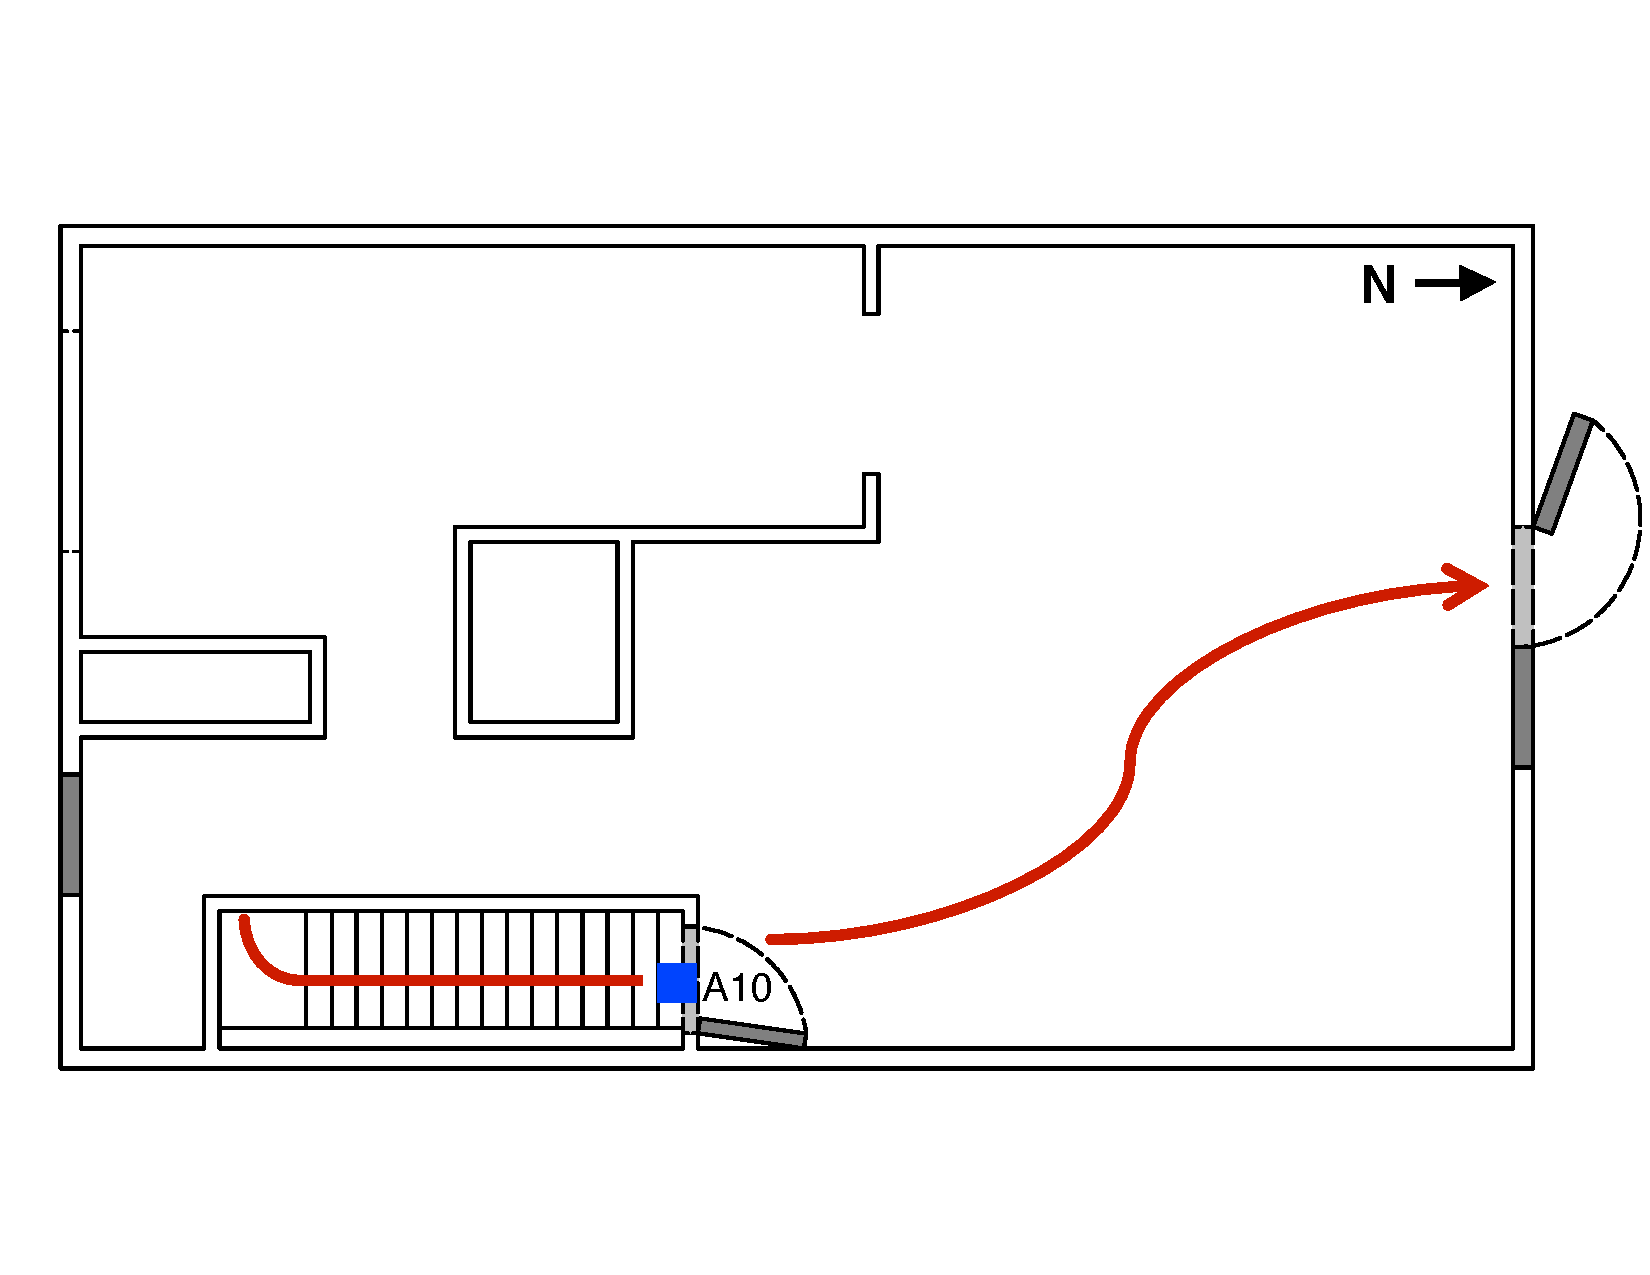
\includegraphics[width=\columnwidth]{../Figures/Floor_Plans/Specific_Tests/West_Hose_Test_2nd_Floor_Annotated}
	\\~\\
	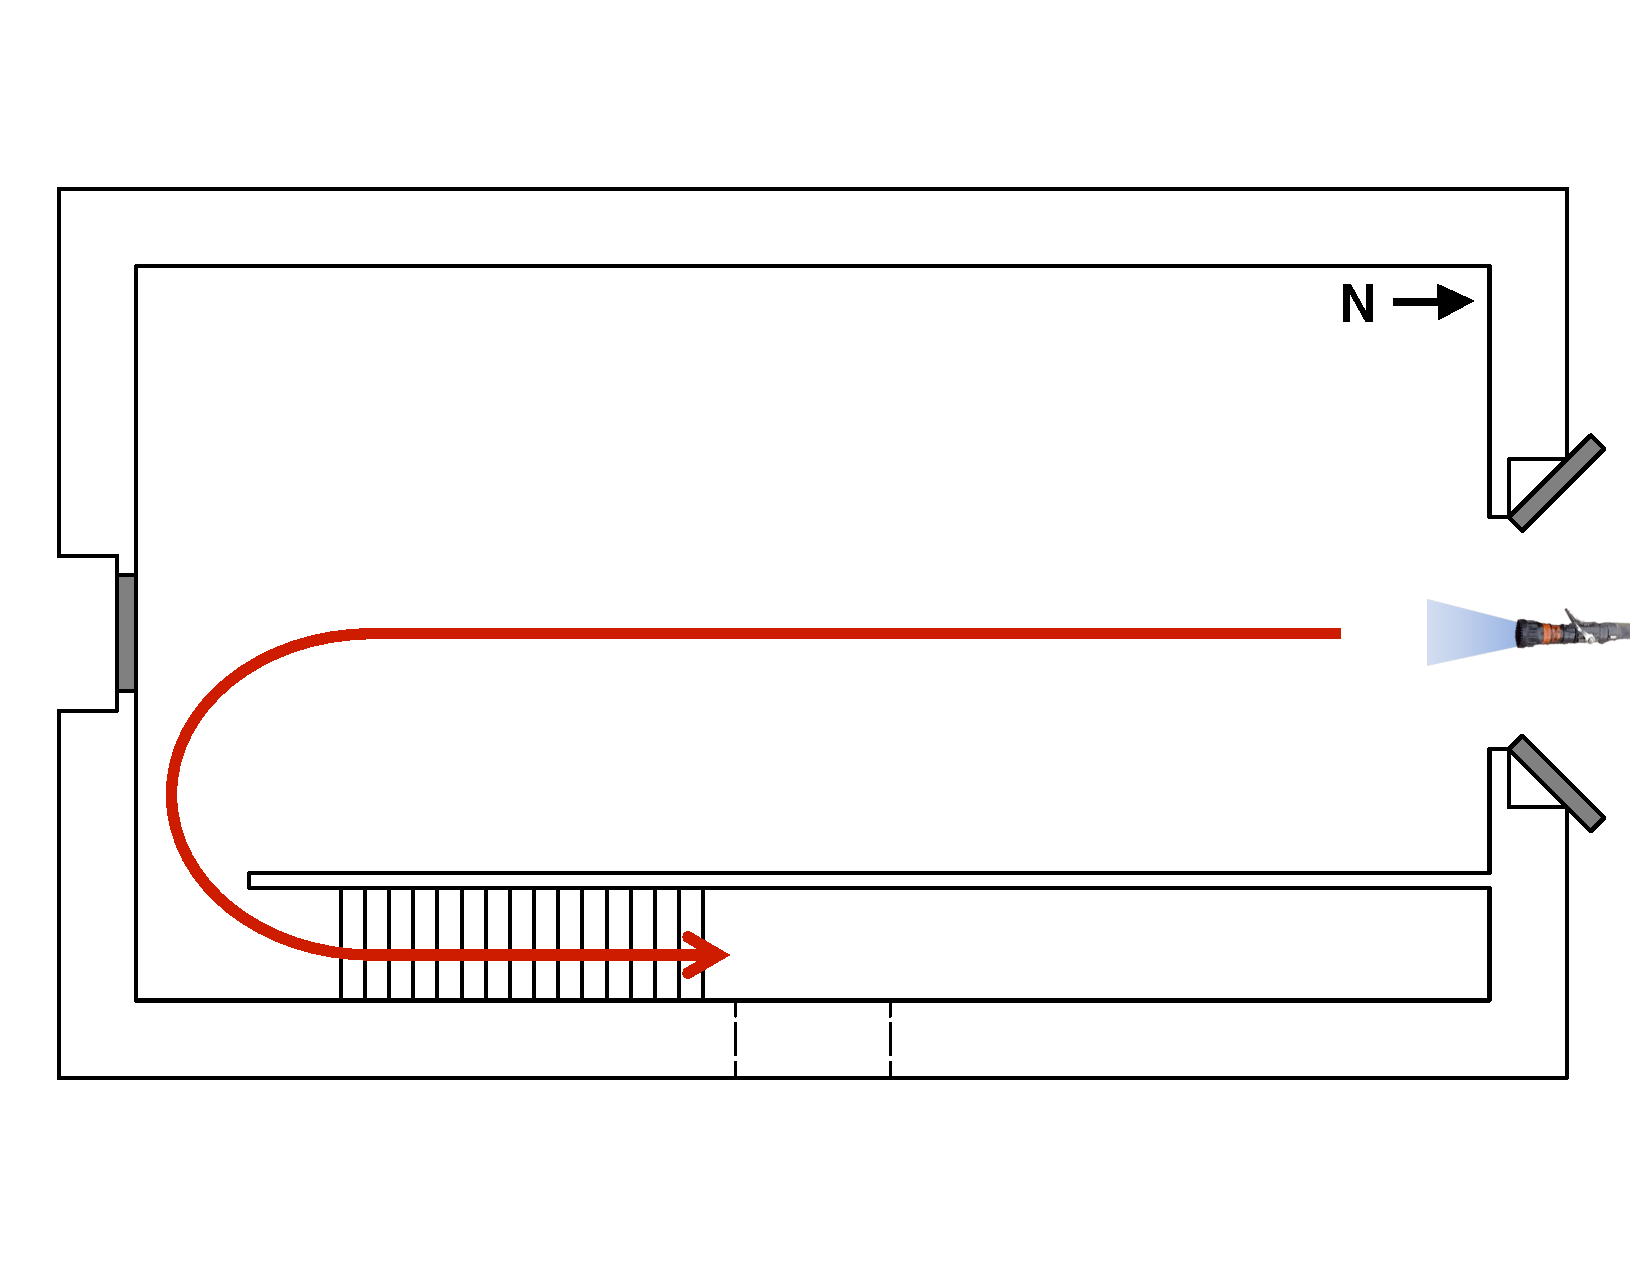
\includegraphics[width=\columnwidth]{../Figures/Floor_Plans/Specific_Tests/West_Hose_Test_19_1st_Floor_Annotated}
	\caption[Plan view of the West Structure setup for Tests 17 and 19.]{Plan view of the second floor (top) and first floor (bottom) setup in the West Structure for Tests 17 and 19. The approximate location of water flow (nozzle graphic), the direction of the established flow path (red line), and the approximate location of A10 (blue square). On the second floor, the stairwell door and north side, west double door were opened and closed at certain instances during the tests; the flow path was considered fully established when both doors were in the opened position.}
	\label{fig:flow_path_2}
\end{figure}
\FloatBarrier

\subsection{Monitor Experiments}
\label{sec:monitor_procedure}
Numerous experiments were conducted during three different test series using a monitor equipped with a combination nozzle to flow water at 120~GPM in a straight stream, narrow fog stream, and wide fog stream pattern. One test series, Test 33, occurred in the East Structure, and the two remaining series, Tests 16 and 17, occurred in the West Structure. An additional test series, Test 70, used a combination nozzle and a smooth bore nozzle attached to a monitor to flow water at 180~GPM in a straight stream and solid stream, respectively. Because monitor nozzles are designed to flow water from a set position, water was always applied in a fixed position during the monitor experiments. Thus, the monitor experiments primarily focused on the impact of different hose stream patterns on air movement in a structure.

Test 33 utilized a monitor equipped with a combination nozzle to flow water from Room C of the East Structure to the area above the doorway on the south wall of Room B (Fig.~\ref{fig:test_33_pic}). A plan view of the structure's layout annotated with the approximate location of the bi-directional probes array used to measure gas velocity through an interior doorway (A6) and the general direction of the fully established flow path for Test 33 can be found in Fig.~\ref{fig:east_setup}. The procedure for Test 33 was the simplest of all the test procedures. First, water flowed in a straight stream pattern for 30 seconds, then the stream was changed to a narrow fog for 30 seconds, and finally to a wide fog stream for 30 seconds. An identical process was repeated an additional time.

\begin{figure}[!ht]
	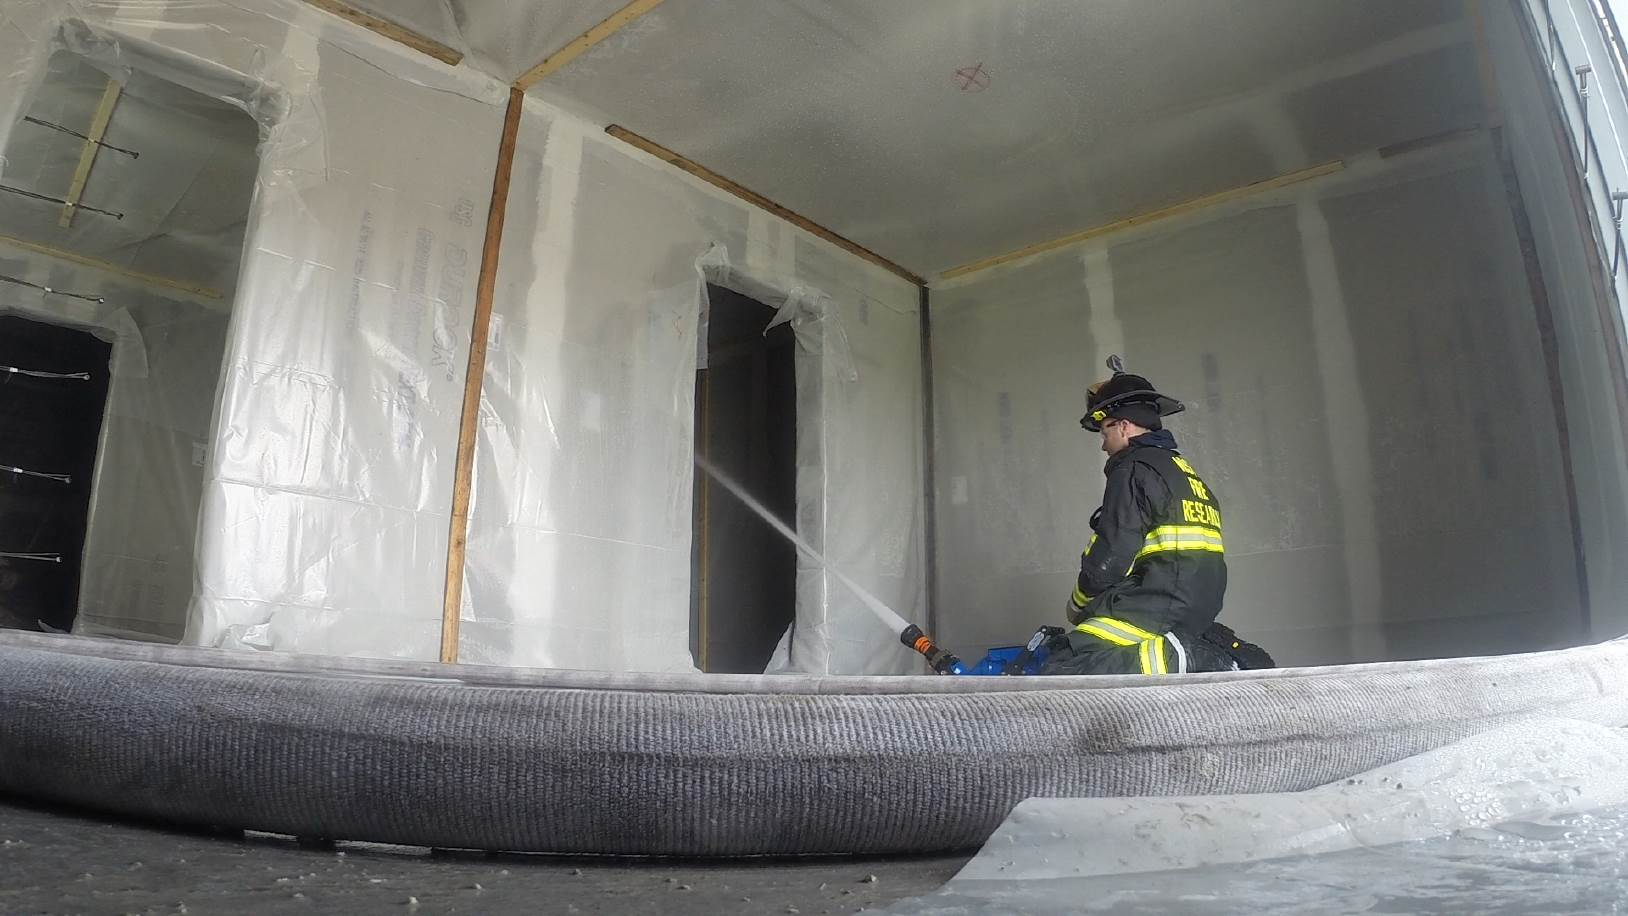
\includegraphics[trim=16cm 6.25cm 9cm 6cm, clip=true, width=4in]{../Figures/Pictures/SS_Room_B_Test_33}
	\\~\\
	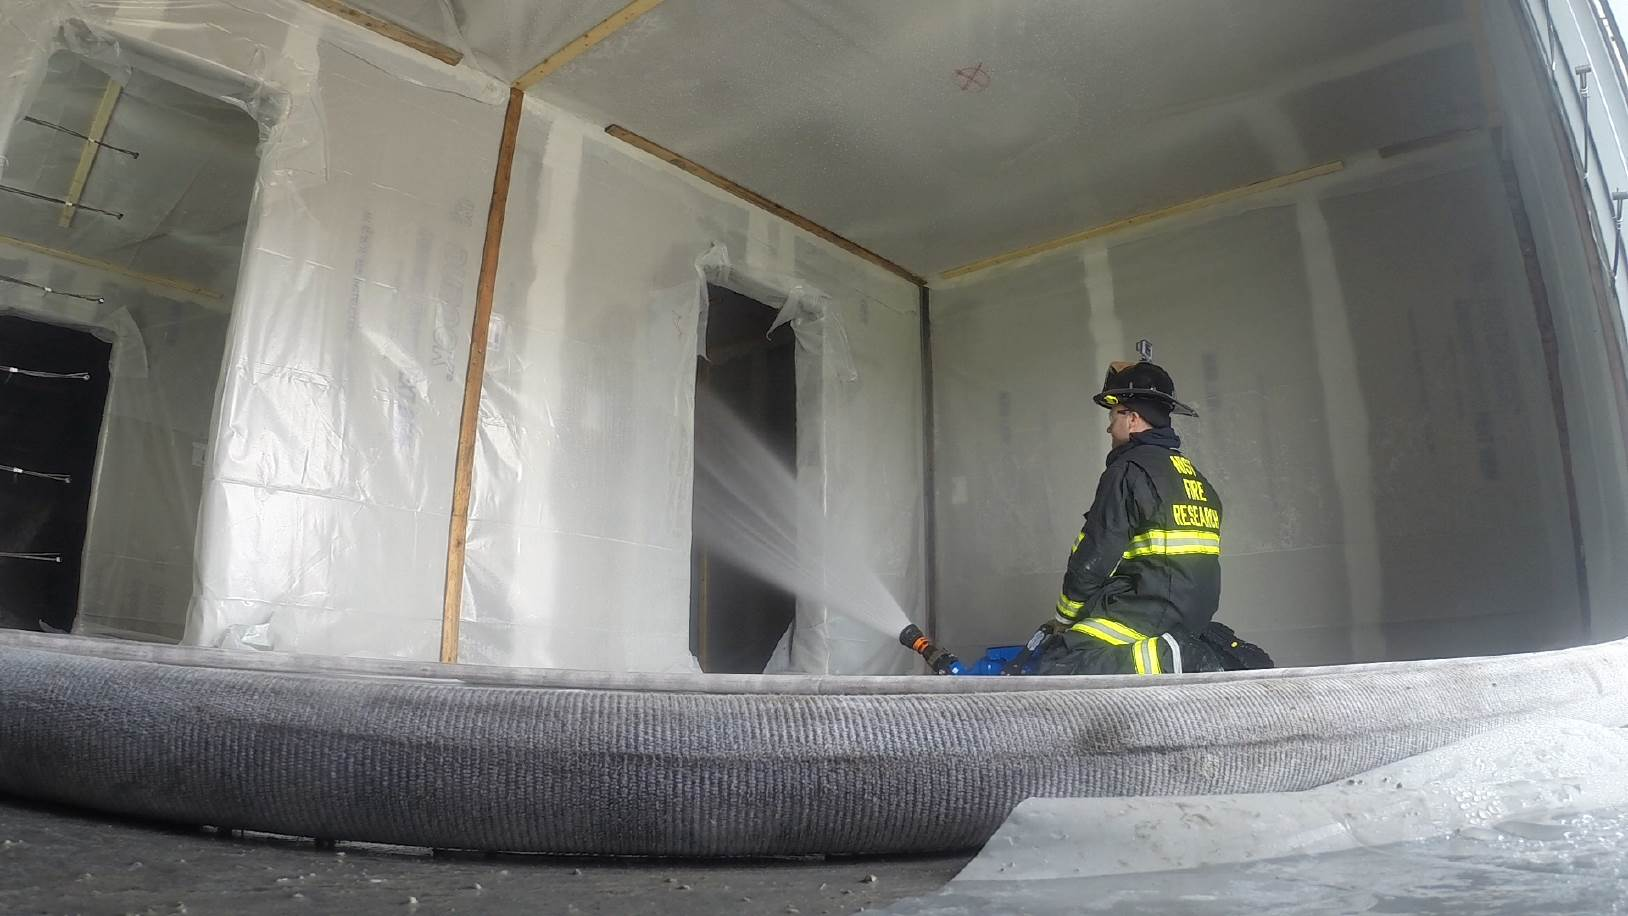
\includegraphics[trim=16cm 6.25cm 9cm 6cm, clip=true, width=4in]{../Figures/Pictures/NF_Room_B_Test_33}
	\\~\\
	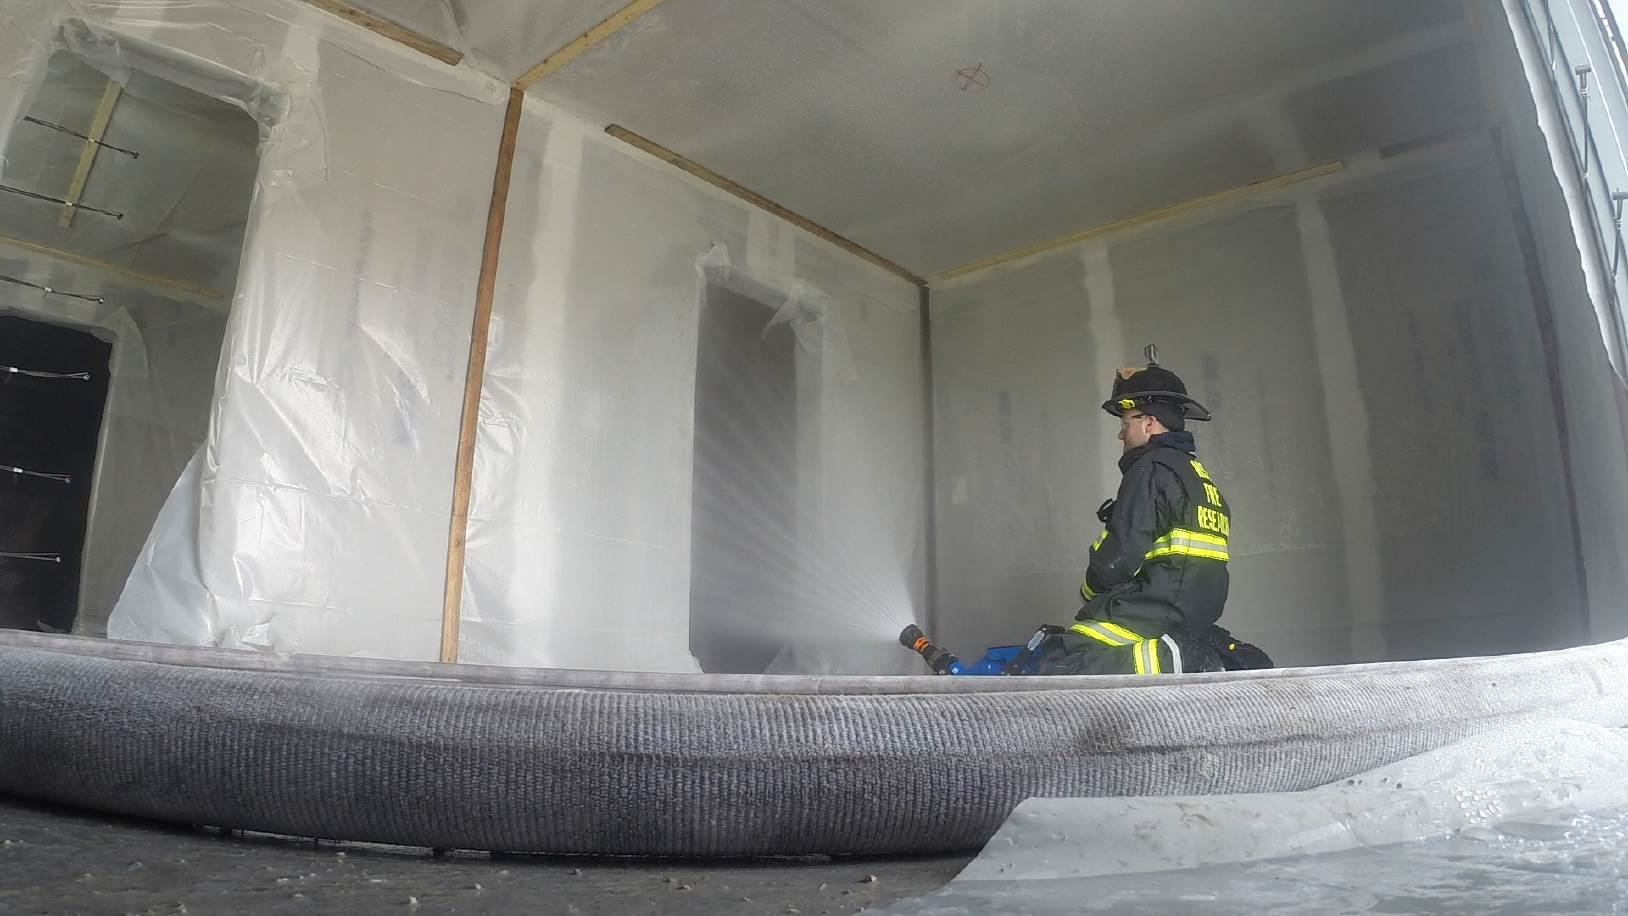
\includegraphics[trim=16cm 6.25cm 9cm 6cm, clip=true, width=4in]{../Figures/Pictures/WF_Room_B_Test_33}
	\caption[Straight stream, narrow fog stream, and wide fog stream during Test 33.]{Water flowing from the monitor in Room C in a straight stream (top), narrow fog stream (middle), and wide fog stream (bottom) pattern aimed at the area above the doorway on the south wall of Room B during Test 33.}
	\label{fig:test_33_pic}
\end{figure}

% Add flow chart? %
Tests 16 and 17 followed identical procedures that involved using a monitor equipped with a combination nozzle to flow water from the north side double doors of the West Structure to the ceiling of the first floor room. The nozzle was aimed at two targets during the series: a ``near" target, located approximately 1.8~m (6~ft) from the interior side of the north wall and a ``far" target, located approximately 3.7~m (12~ft) from the interior side of the north wall. The procedure for each test series began by flowing water in a straight stream pattern at the far target for 60 seconds. After 60 seconds of water flow, the stairwell door was opened. One minute later, the west double door on the north side of the second floor was opened, and water continued to flow for 60 seconds. Next, the water flow was stopped, the two doors were closed, and the procedure was repeated with the monitor aimed at the near target. The entire process was repeated using the narrow fog and wide fog streams. Fig.~\ref{fig:test_16_17_pic} contains images of each type of hose stream aimed at the near and far targets.

\begin{figure}[!ht]
	\minipage{2.15in}
	\begin{center}
		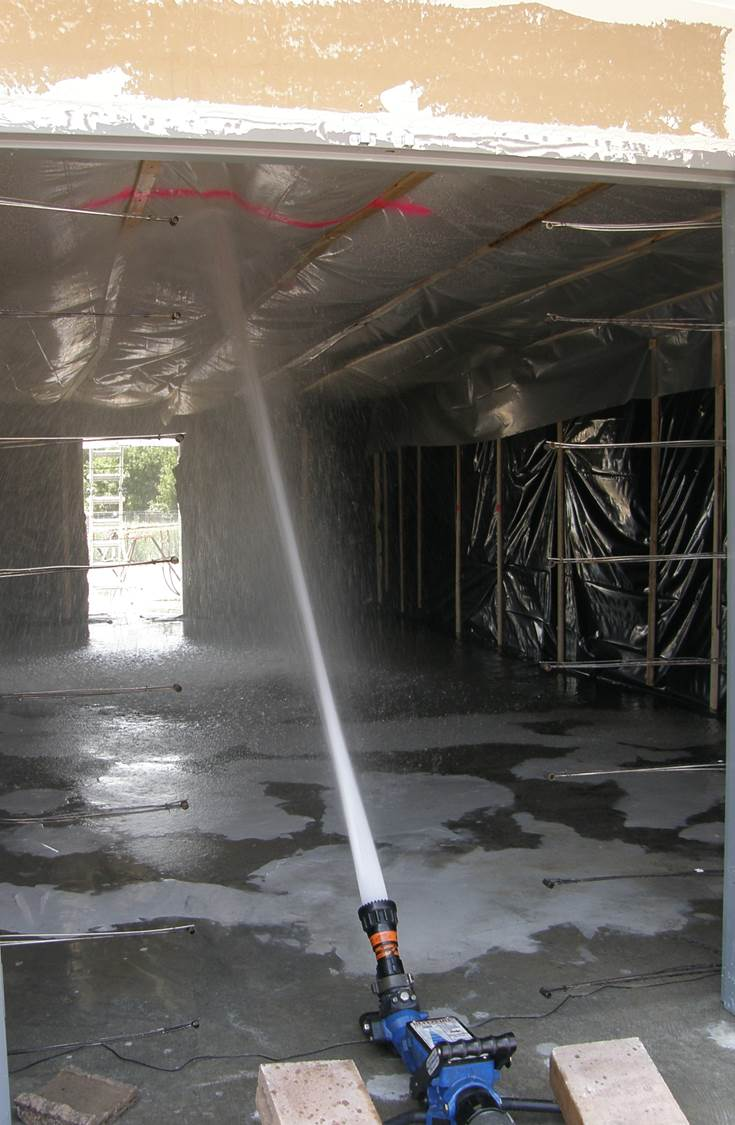
\includegraphics[width=2in]{../Figures/Pictures/SS_near}
	\end{center} 
	\endminipage \hfill
	\minipage{2.15in}
	\begin{center}
		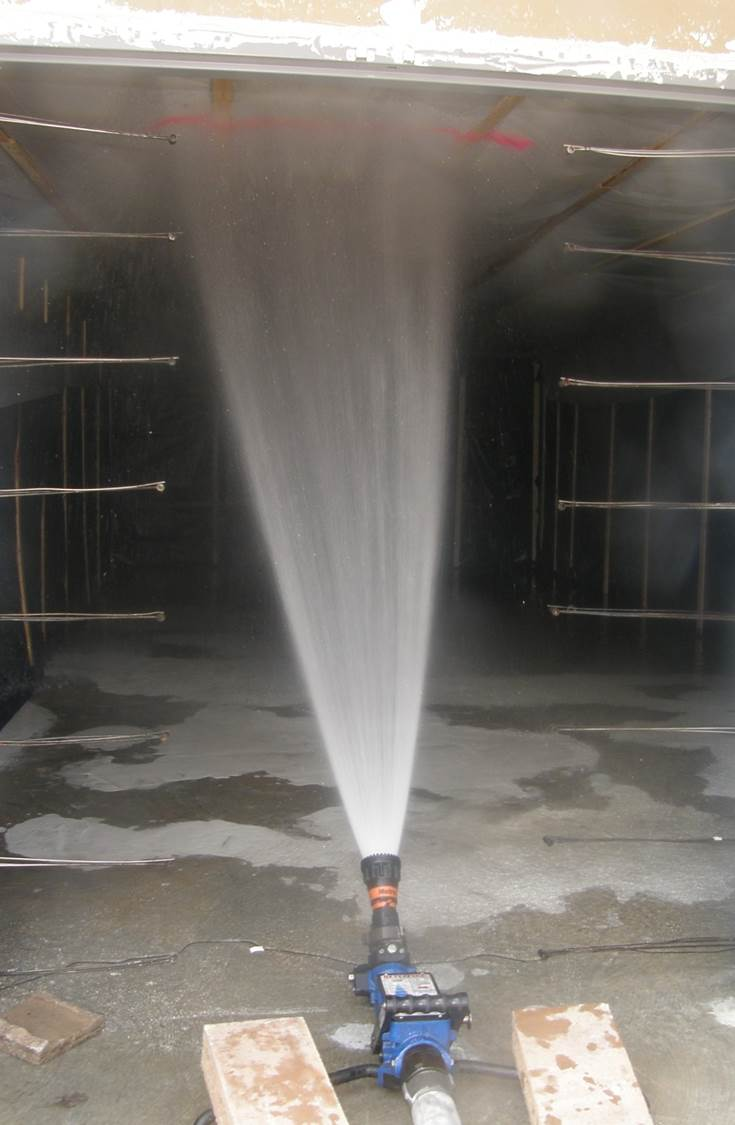
\includegraphics[width=2in]{../Figures/Pictures/NF_near}
	\end{center}
	\endminipage \hfill
	\minipage{2.15in}
	\begin{center}
		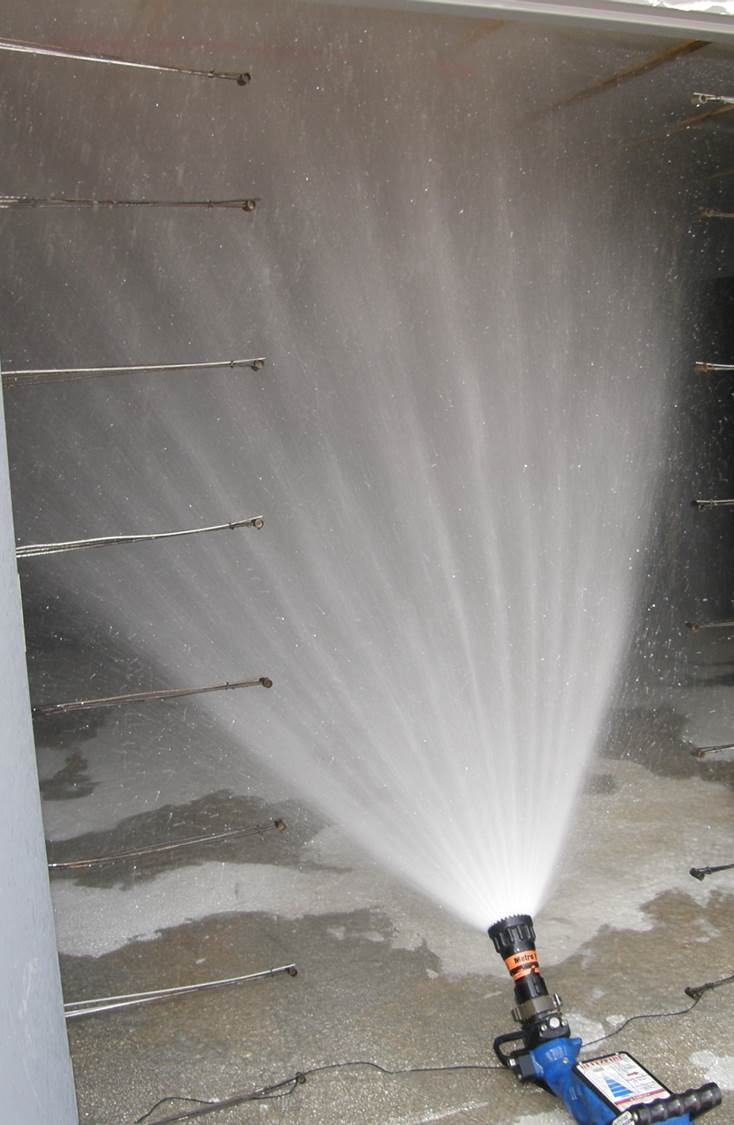
\includegraphics[width=2in]{../Figures/Pictures/WF_near}
	\end{center}
	\endminipage \hfill
	\vspace{0.15in}
	\minipage{2.15in}
	\begin{center}
		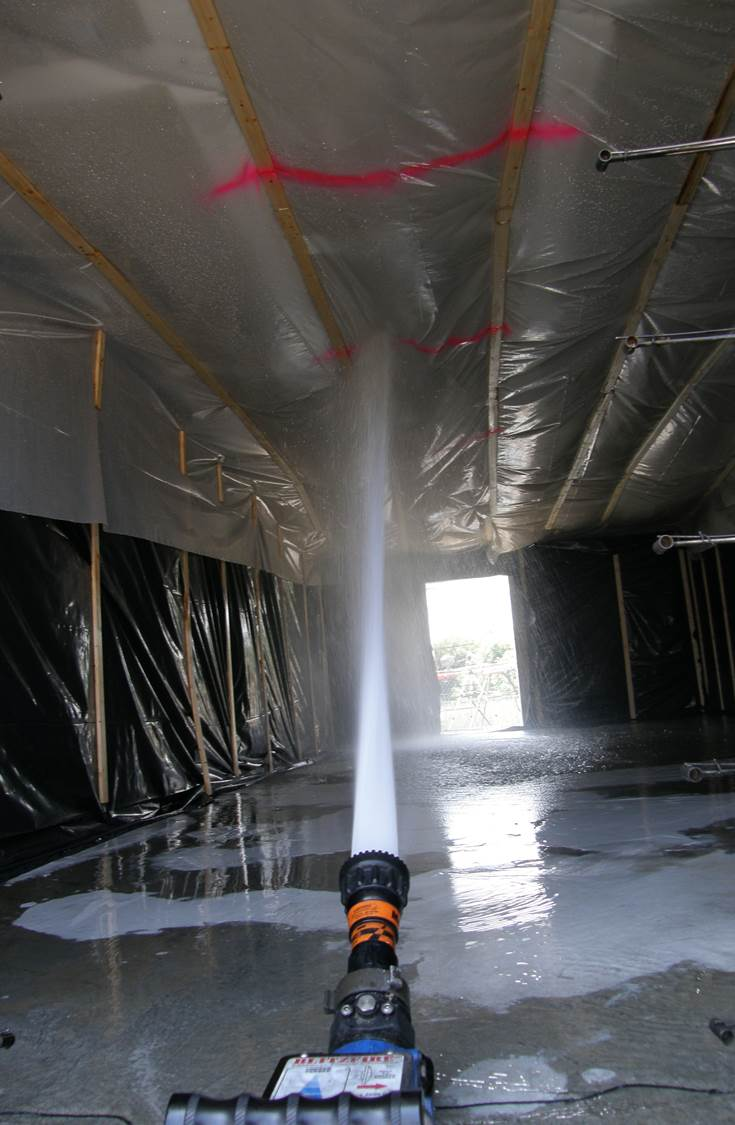
\includegraphics[width=2in]{../Figures/Pictures/SS_far}
	\end{center} 
	\endminipage \hfill
	\minipage{2.15in}
	\begin{center}
		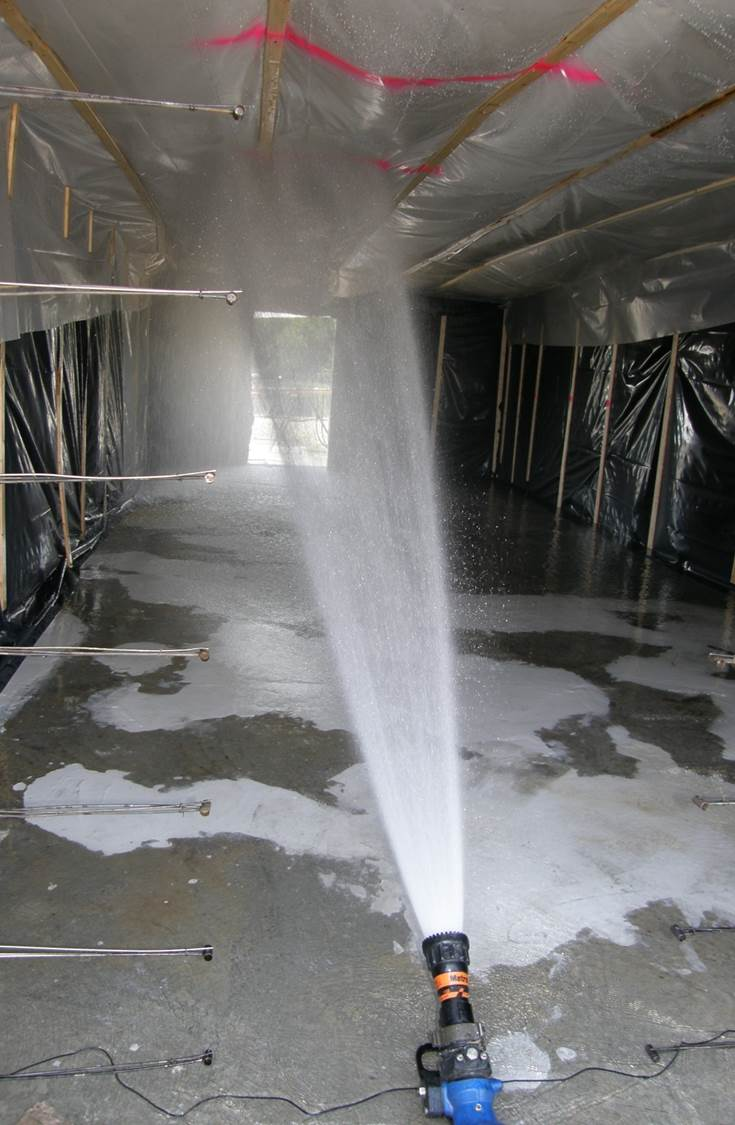
\includegraphics[width=2in]{../Figures/Pictures/NF_far}
	\end{center}
	\endminipage \hfill
	\minipage{2.15in}
	\begin{center}
		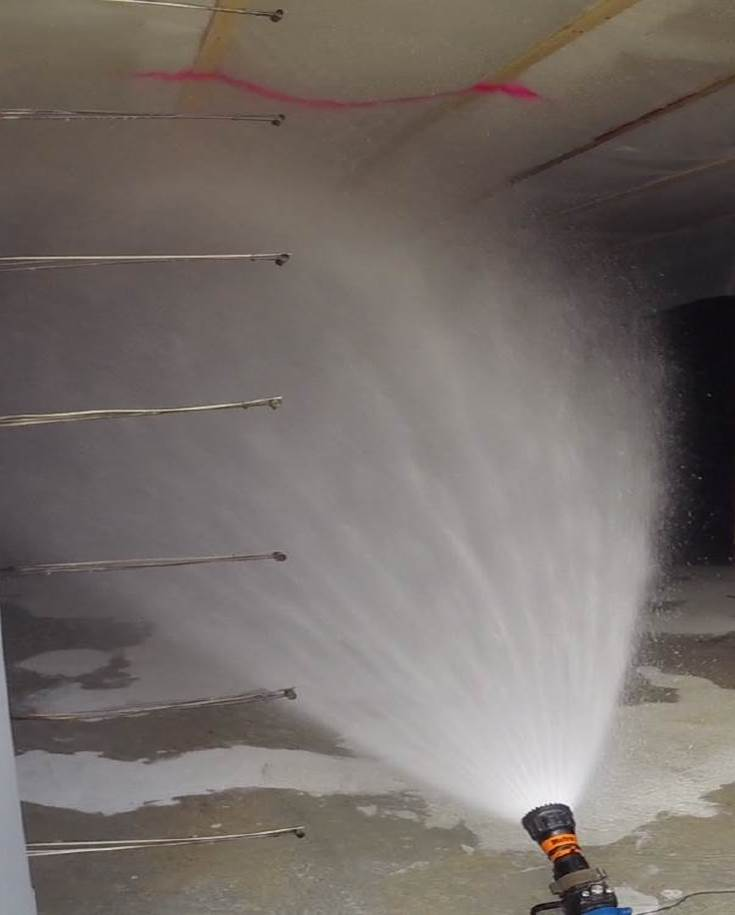
\includegraphics[width=2in]{../Figures/Pictures/WF_far}
	\end{center}
	\endminipage \hfill
	\caption[Straight stream, narrow fog stream, and wide fog stream aimed at the near and far targets in the West Structure.]{Straight stream (left column), narrow fog stream (middle column), and wide fog stream (right column) aimed at ``near" target (top row) and ``far" target (bottom row) during the monitor experiments in the West Structure.}
	\label{fig:test_16_17_pic}
\end{figure}
\FloatBarrier

Test 70 studied the differences in air movement caused by a solid stream from a smooth bore nozzle and straight stream from a combination nozzle attached to a monitor aimed at the same near and far targets used during Tests 16 and 17. The stairwell door was opened for the entire test series. The test series began by flowing water in a straight stream from a combination nozzle aimed at the near target. Then, the west double door on the second floor was opened. After 60 more seconds of flow, the nozzle was closed to stop flow for 30 seconds. The nozzle was opened for 60 seconds and then closed for 30 seconds two additional times. Then, the monitor was aimed at the far target, and the procedure was repeated. This entire process was repeated using the solid stream from the smooth bore nozzle. Fig.~\ref{fig:test_70_pic} contains images of the straight stream from the combination nozzle and solid stream from the smooth bore nozzle during Test 70.

\begin{figure}[!ht]
	\minipage{2.15in}
	\begin{center}
		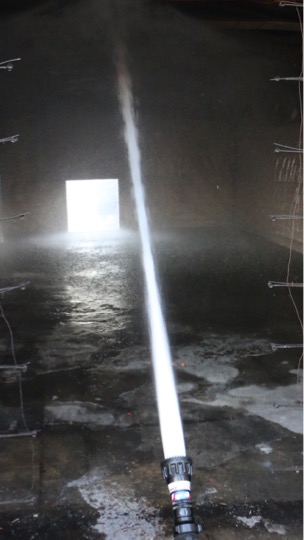
\includegraphics[width=2in]{../Figures/Pictures/SS_70}
	\end{center} 
	\endminipage
	\minipage{2.15in}
	\begin{center}
		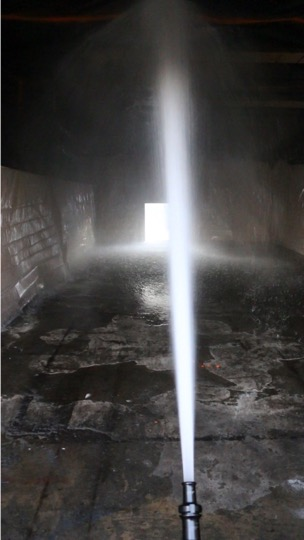
\includegraphics[width=2in]{../Figures/Pictures/SB_70}
	\end{center}
	\endminipage
	\caption[Straight stream from combination nozzle and solid stream from smooth bore nozzle during Test 70.]{Straight stream (left) from combination nozzle and solid stream (right) from smooth bore nozzle during Test 70.}
	\label{fig:test_70_pic}
\end{figure}
\FloatBarrier

\subsection{Handline Experiments}
\label{sec:handline_procedure}
Numerous experiments were conducted during three different test series using a 1.75~in handline with a combination nozzle to flow water in a straight stream, narrow fog stream, and wide fog stream pattern. One test series, Test 34, occurred in the East Structure, and the remaining series, Tests 18 and 19, occurred in the West Structure. All three test series primarily focused on the impact of different hose stream and water application pattern selections on air movement in a structure. 

Test 34 utilized a 1.75~in handline equipped with a combination nozzle to flow water from Room C of the East Structure into Room B (Fig.~\ref{fig:test_34_pic}). The layout of the structure was identical to the layout described above in Section~\ref{sec:monitor_procedure} and shown in Fig.~\ref{fig:east_setup}. The procedure for Test 34 began by flowing water in a straight stream aimed at the ceiling of Room B for 30 seconds in a fixed position. After 30 seconds, the nozzle was rotated in the clockwise direction for 30 seconds. Then, the nozzle was aimed at the south doorway of Room B and water was applied for 30 seconds in a fixed position followed by 30 seconds in a clockwise pattern. This process was repeated for narrow fog and wide fog streams. Then, the entire procedure was repeated for the three types of streams being applied in the fixed and counter-clockwise pattern.

\begin{figure}[!ht]
	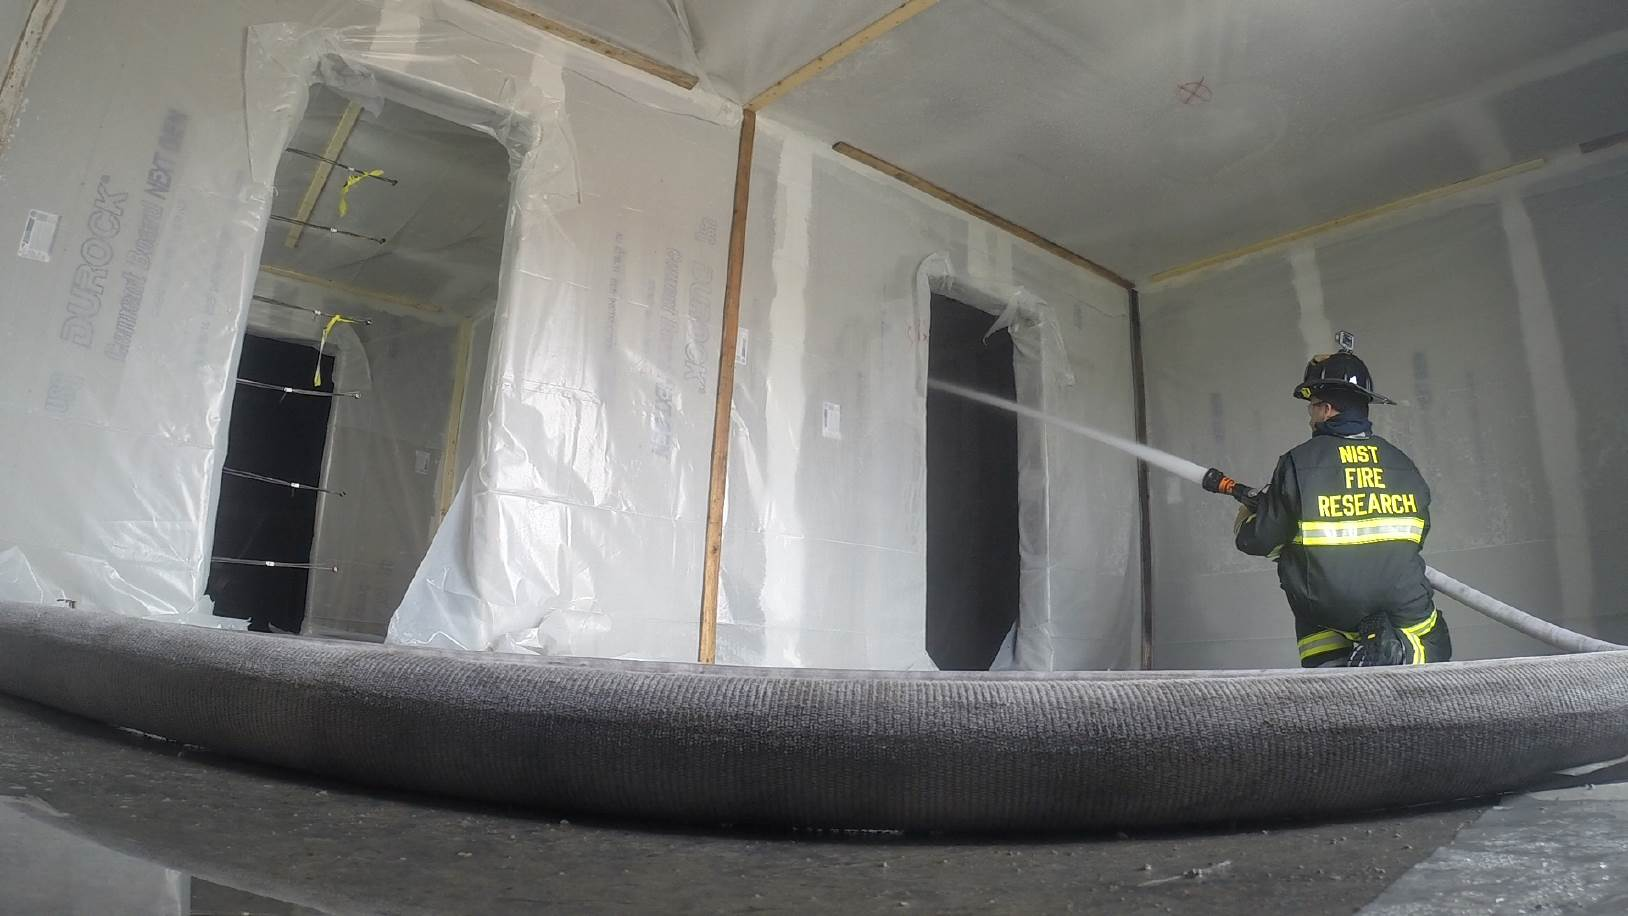
\includegraphics[trim=23cm 6.5cm 4cm 6cm, clip=true, width=3.75in]{../Figures/Pictures/SS_Room_B_Test_34}
	\\~\\
	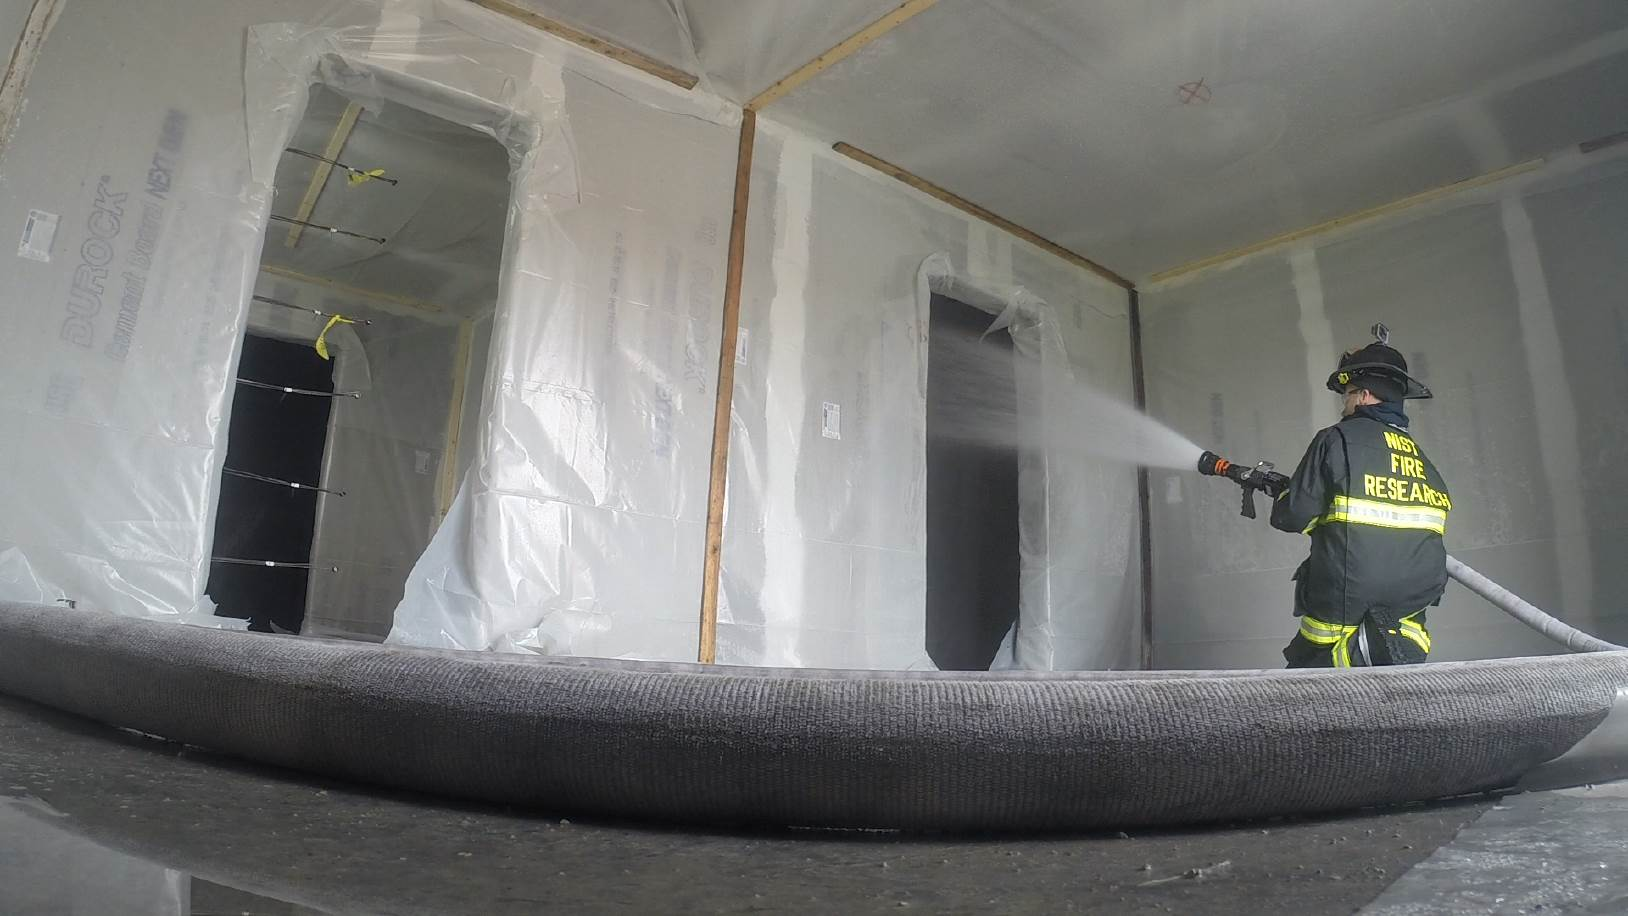
\includegraphics[trim=23cm 6.5cm 4cm 6cm, clip=true, width=3.75in]{../Figures/Pictures/NF_Room_B_Test_34}
	\\~\\
	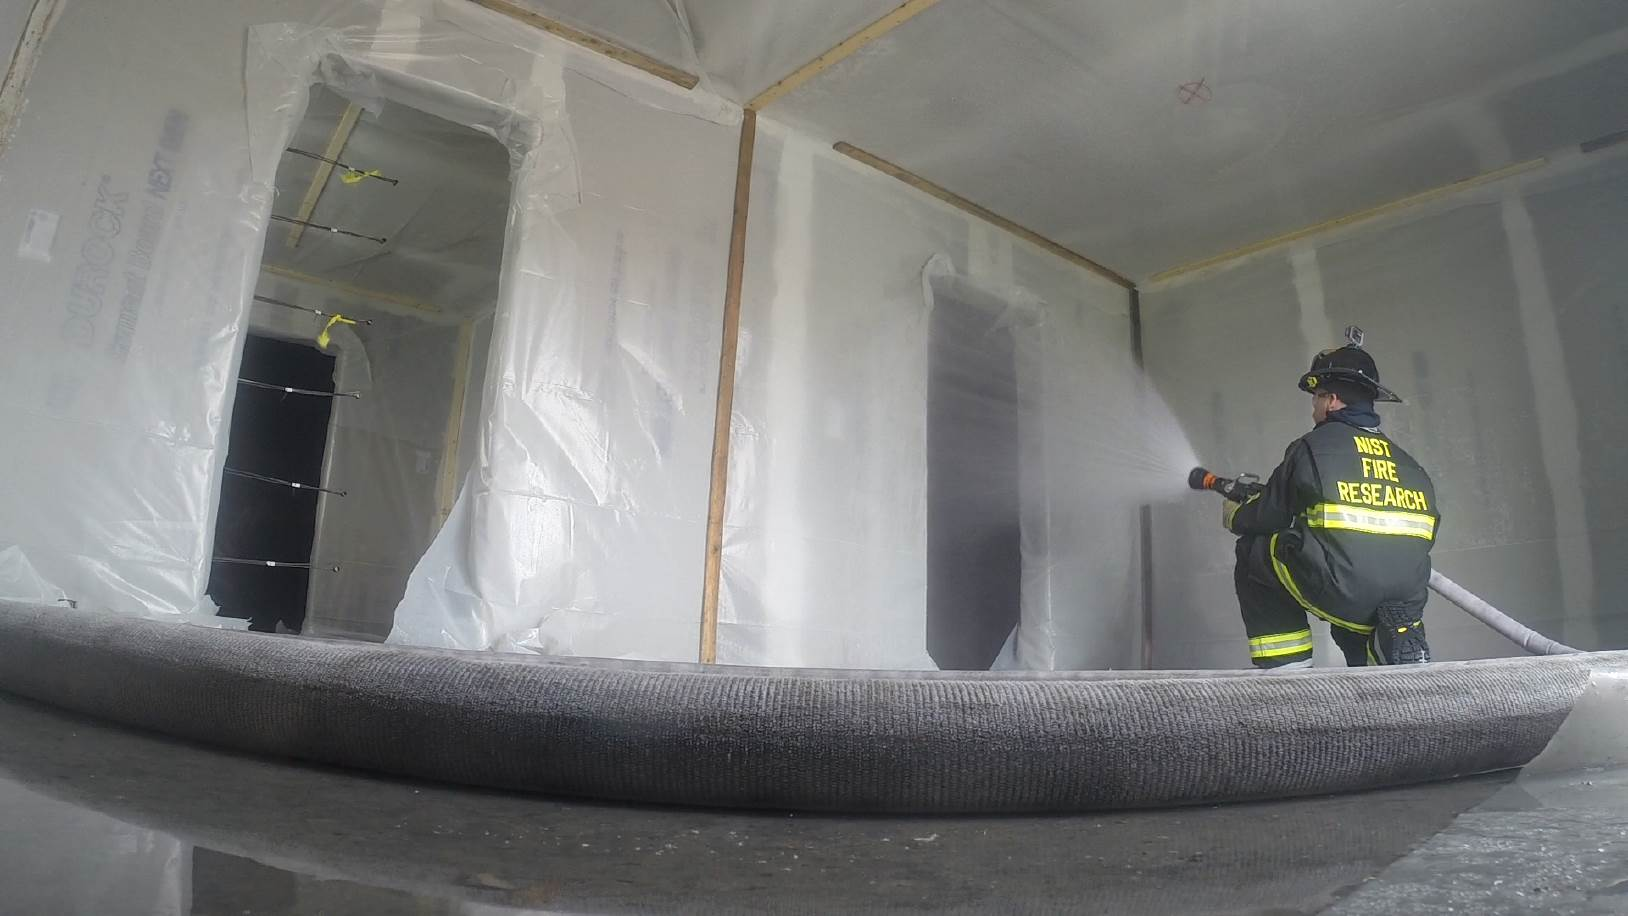
\includegraphics[trim=23cm 6.5cm 4cm 6cm, clip=true, width=3.75in]{../Figures/Pictures/WF_Room_B_Test_34}
	\caption[Straight stream, narrow fog stream, and wide fog stream during Test 34.]{Straight stream (top), narrow fog stream (middle), and wide fog stream (bottom) aimed at the south doorway of Room B during Test 34.}
	\label{fig:test_34_pic}
\end{figure}

% Where was the handline aimed? Add flow chart? %
Tests 18 and 19 followed identical procedures that involved using a 1.75~in handline equipped with a combination nozzle to flow water from the north side double doors of the West Structure into the first floor room. For every experiment during the two tests, the water stream was aimed at the south side wall of the first floor. The difference between Tests 18 and 19 is that Test 18 contained the same flow path configuration presented in Fig.~\ref{fig:flow_path_1}, while Test 19 contained the same flow path configuration presented in Fig.~\ref{fig:flow_path_2}. Each test series began by using a straight stream to flow water in a fixed position. After 60 seconds of water flow, the stairwell door was opened. One minute later, the north side, west double door on the second floor was opened, and water continued to flow for 60 seconds. Next, the water flow was stopped, the two doors were closed, and the process was repeated three additional times for the sweeping, clockwise, and counterclockwise application patterns. This entire procedure was repeated using narrow fog and wide fog streams. Fig.~\ref{fig:test_18_pic} contains an image of a straight stream pattern being applied during Test 18 with the flow path fully established.

\begin{figure}[!ht]
	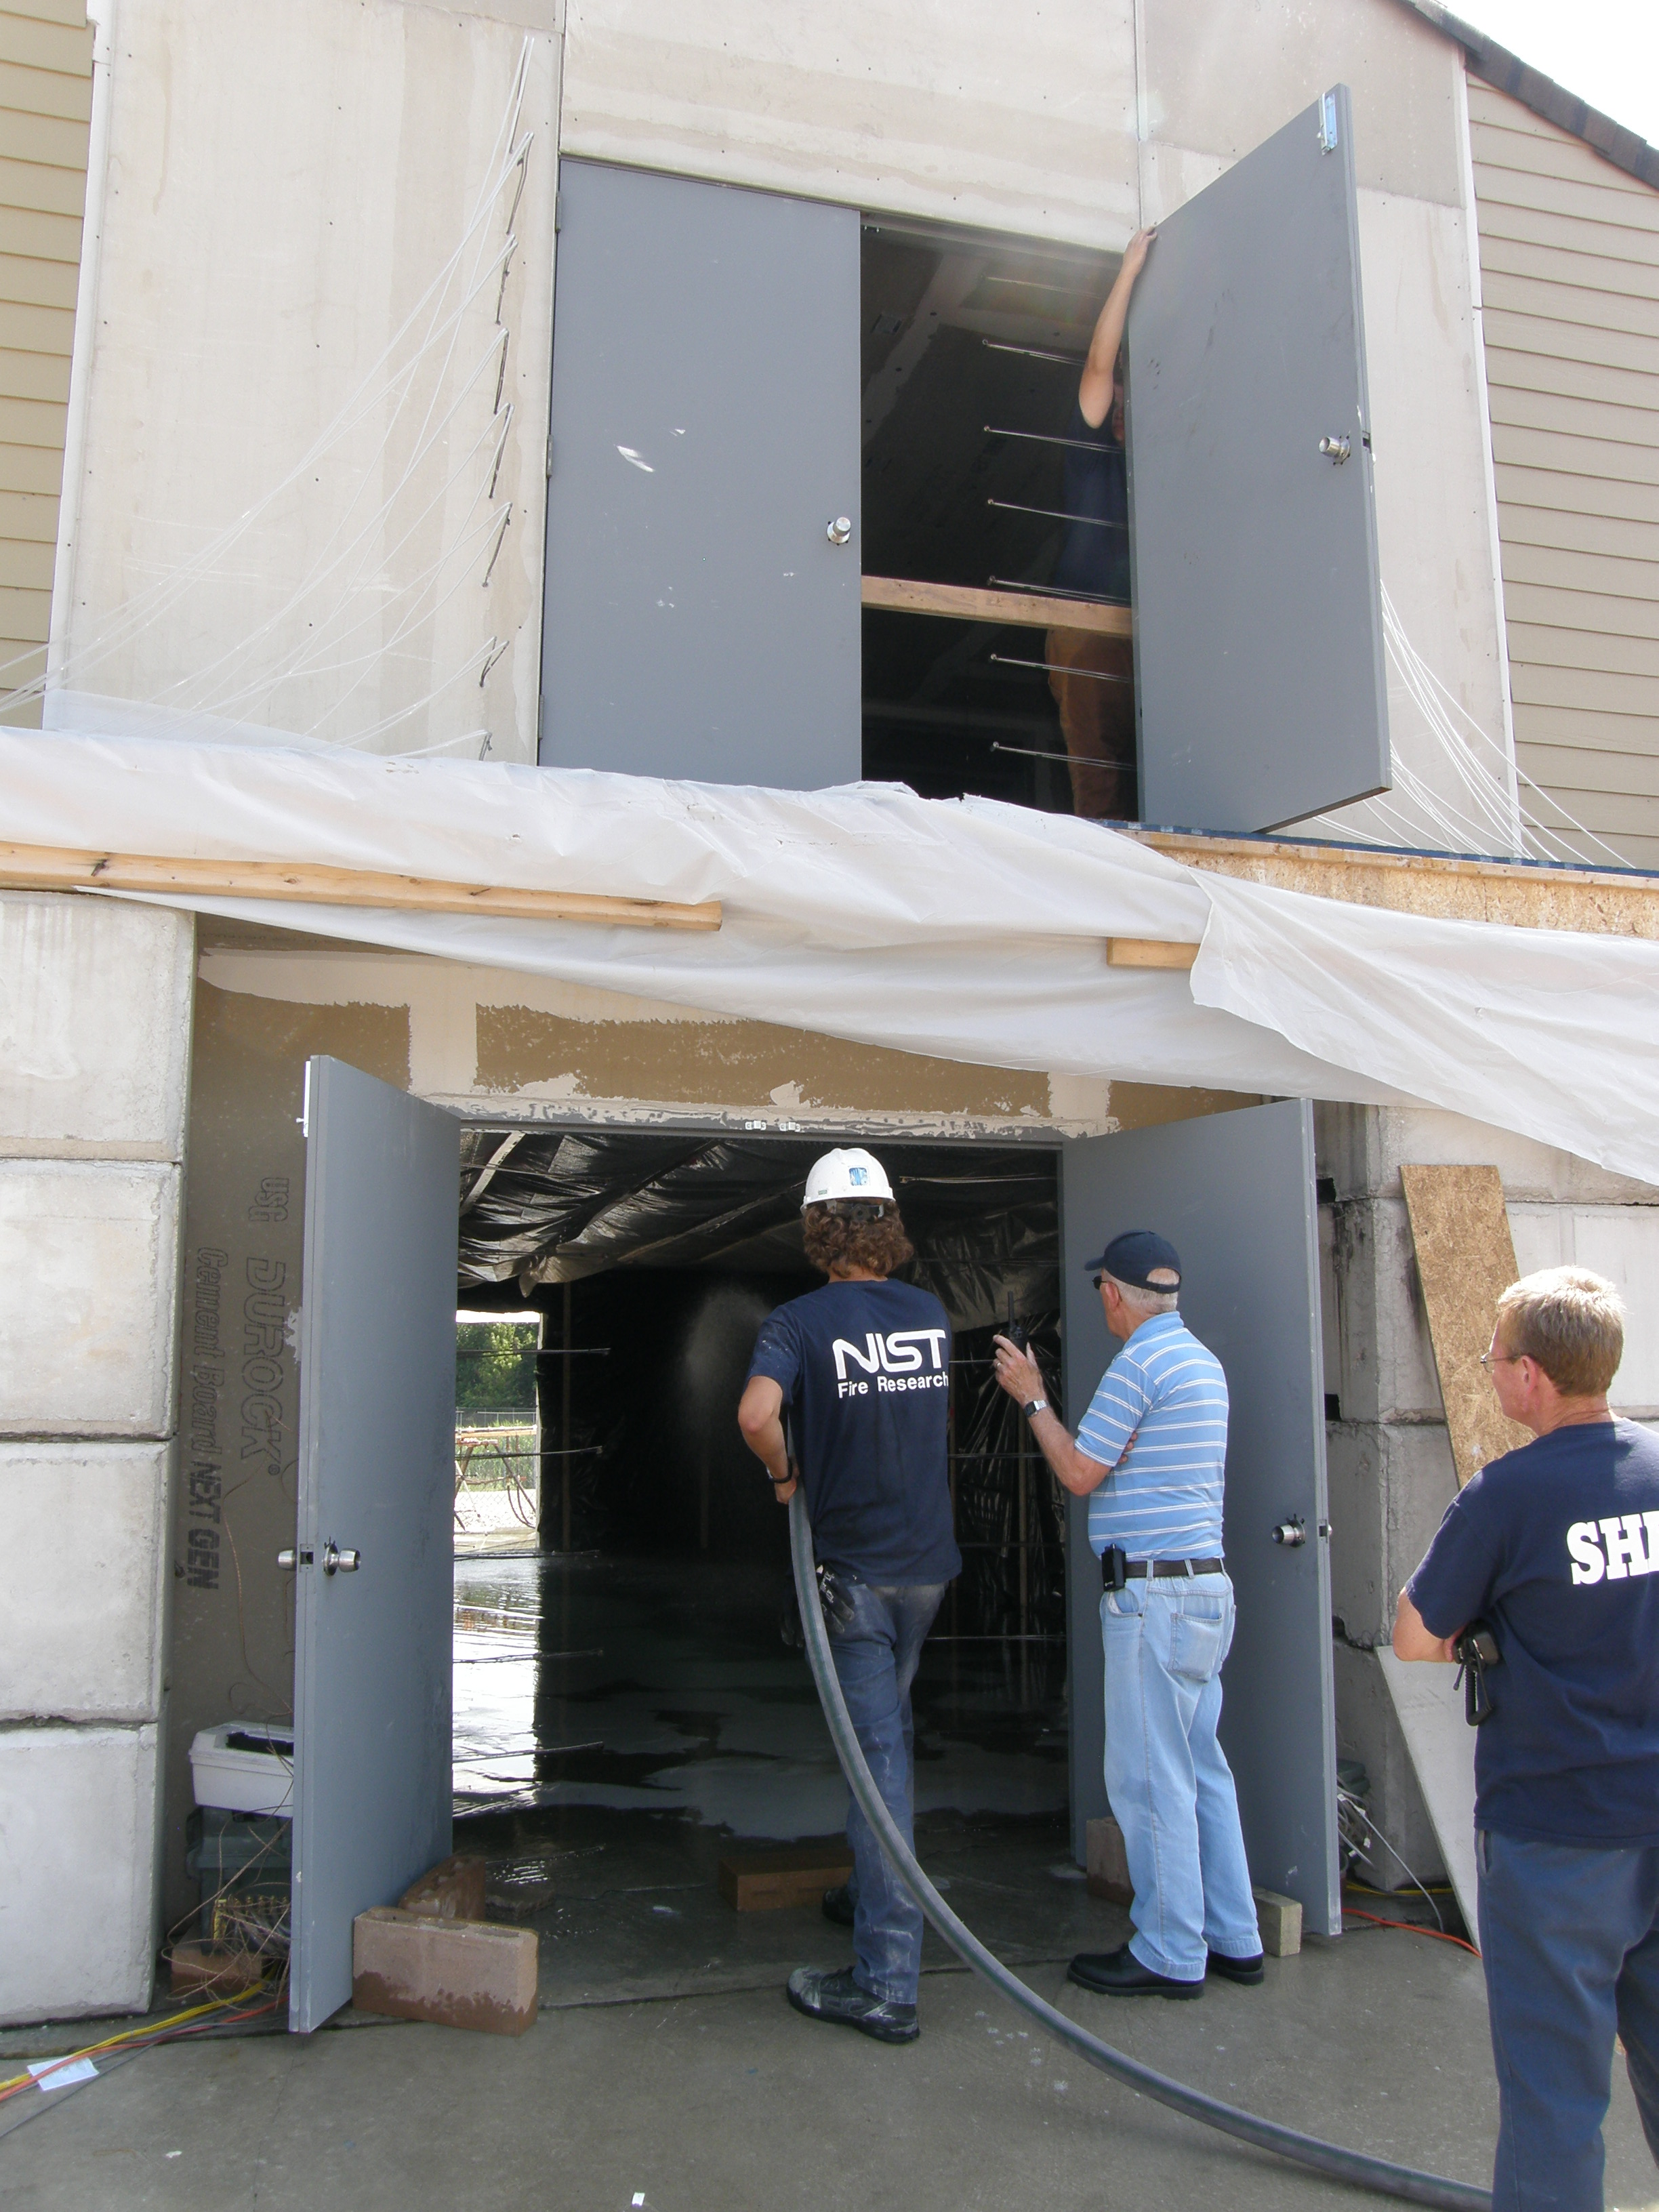
\includegraphics[width=4.25in]{../Figures/Pictures/Test_18}
	\caption[North side of West Structure containing a fully established flow path during Test 18.]{North side of West Structure containing a fully established flow path while water is flowed in a straight stream pattern during Test 18.}
	\label{fig:test_18_pic}
\end{figure}
\FloatBarrier

% ===========
% = RESULTS =
% ===========

\chapter{Results and Discussion}
\label{chap:results}
In the following sections, the measurements will be presented in graphic and tabular form. In the graphs, an error bar will represent the estimated uncertainty of the measurement. In the tables, the uncertainty will be included in the caption of the table.

\section{Monitor Experiments}
\label{sec:monitor_results}

Fig.~\ref{fig:Test_16_A10_Avgs} contains a plot of the average velocity measured by the bi-directional probes at A10 for the straight, narrow fog, and wide fog stream patterns aimed at the near and far targets during Test 16. Similar plots that were generated using measurements obtained from the bi-directional probes at A10 during Test 17 and measurements obtained from the bi-directional probes at A6 during Test 33 are presented in Appendix~\ref{sec:monitor_figs}.

\begin{figure}[!ht]
	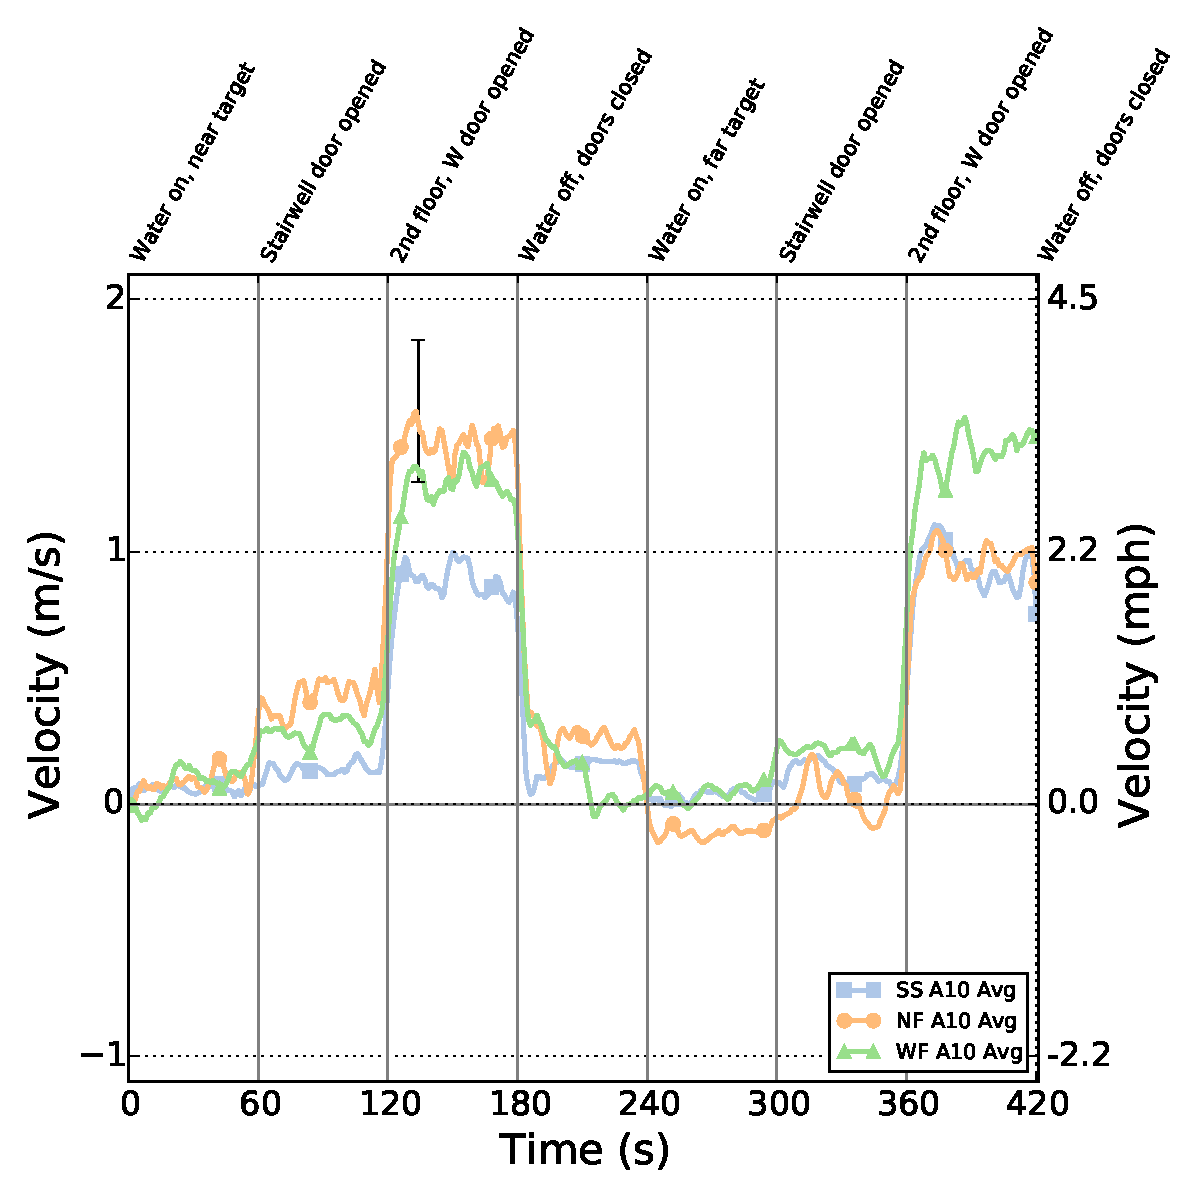
\includegraphics[width=\columnwidth]{../Figures/Plots/Test_16_West_063014_BDP_A10_stream_avgs}
	\caption{Average velocity through stairwell door during Test 16 for three hose stream patterns.}
	\label{fig:Test_16_BDP_A10_Avg_All}
\end{figure}
\FloatBarrier

For every hose stream and target location combination during the monitor experiments, there was always significant air movement (gas velocity greater than 0.5 m/s) through the interior doorway while the flow path was fully established. Table~\ref{table:all_mon_vel_avgs} lists the average velocity measured by the bi-directional probes array at the interior doorway when the flow path was fully established for each hose stream and target location combination studied during Tests 16, 17, and 33.   

\begin{table}[!ht]
\caption{Average air velocity (m/s) through interior doorway when flow path was fully established for each monitor experiment}
\begin{tabular}{lccccc}
\toprule
 & \multicolumn{2}{c}{\underline{Test 16}} & \multicolumn{2}{c}{\underline{Test 17}} & \underline{Test 33}
\\
% \textbf{Stream} & \textbf{Near} & \textbf{Far} & \textbf{Near} & \textbf{Far} 
\textbf{Stream} & 
\begin{tabular}{@{}c@{}} \textbf{Near} \\ \textbf{Target} \\ \end{tabular} & \begin{tabular}{@{}c@{}} \textbf{Far} \\ \textbf{Target} \\ \end{tabular} &
\begin{tabular}{@{}c@{}} \textbf{Near} \\ \textbf{Target} \\ \end{tabular} & \begin{tabular}{@{}c@{}} \textbf{Far} \\ \textbf{Target} \\ \end{tabular} &
\begin{tabular}{@{}c@{}} \textbf{Room B} \\ \textbf{South Doorway} \\ \end{tabular}
\\ 
\midrule
\textit{Straight} & 0.9 $\pm0.1$ & 0.9 $\pm0.2$ & 0.7 $\pm0.1$ & 0.7 $\pm0.2$ & -0.3 $\pm0.1$
\\ \multicolumn{6}{c}{} \\
\textit{Narrow Fog} & 0.9 $\pm0.2$ & 1.4 $\pm0.2$ & 0.7 $\pm0.2$ & 0.7 $\pm0.1$ & 1.0 $\pm0.6$
\\ \multicolumn{6}{c}{} \\
\textit{Wide Fog} & 1.2 $\pm0.2$ & 1.3 $\pm0.2$ & 0.9 $\pm0.2$ & 0.8 $\pm0.2$ & 2.4 $\pm0.3$
\\ \midrule
 & \multicolumn{2}{c}{\underline{Test 70}} & \multicolumn{3}{c}{} \\
\textbf{Stream} &
\begin{tabular}{@{}c@{}} \textbf{Near} \\ \textbf{Target} \\ \end{tabular} & 
\begin{tabular}{@{}c@{}} \textbf{Far} \\ \textbf{Target} \\ \end{tabular} &
\multicolumn{3}{c}{} 
\\
\midrule
\textit{Straight} & 1.7 $\pm0.4$ & 1.9 $\pm0.5$ & \multicolumn{3}{c}{} 
\\ \multicolumn{6}{c}{} \\
\textit{Smooth Bore} & 1.7 $\pm0.5$ & 2.0 $\pm0.5$ & \multicolumn{3}{c}{}
\\
\bottomrule
\end{tabular}
\label{table:all_mon_vel_avgs}
\end{table}
\FloatBarrier

**** Discuss tabulated results, main point being fogs move more air than straight ****

\section{Handline Experiments}
\label{sec:handline_results}

Fig.~\ref{fig:Test_18_BDP_A10_Avg_All} contains a plot of the average velocity measured by the bi-directional probes at A10 for the straight, narrow fog, and wide fog stream patterns being applied in a fixed position, a sweeping pattern, a clockwise rotation, and counter clockwise rotation during Test 18. Similar plots that were generated using measurements obtained from the bi-directional probes at A10 during Test 19 and measurements obtained from the bi-directional probes at A6 during Test 34 are presented in Appendix~\ref{sec:handline_figs}.

\begin{figure}[!ht]
	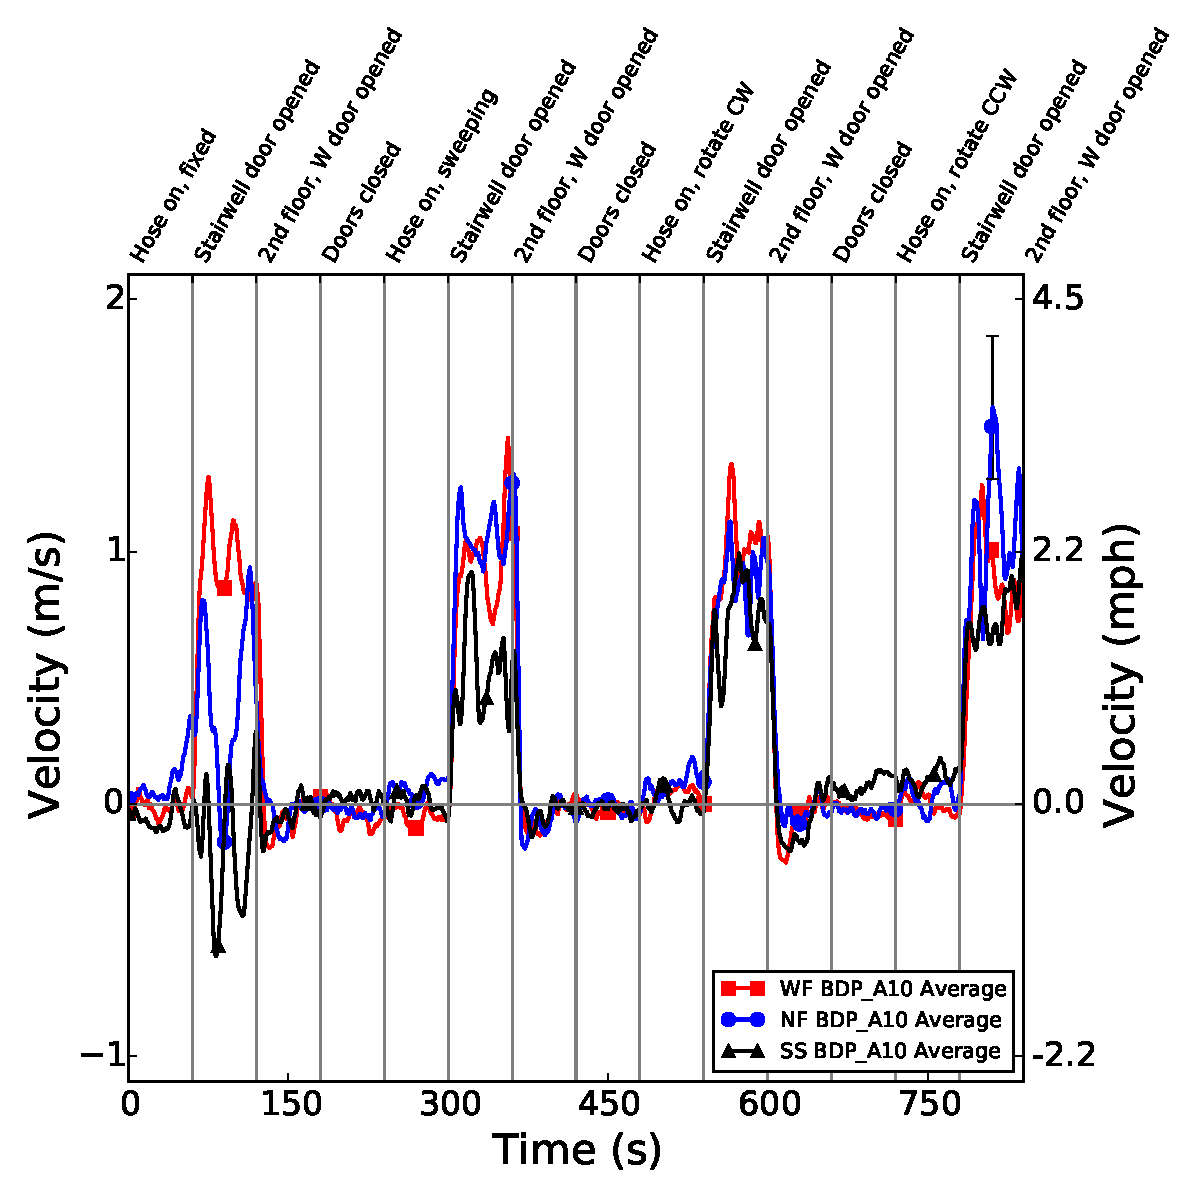
\includegraphics[width=\columnwidth]{../Figures/Plots/Test_18_West_063014_BDP_A10_stream_avgs}
	\caption{Average velocity through stairwell door during Test 18 for the three hose stream patterns.}
	\label{fig:Test_18_BDP_A10_Avg_All}
\end{figure}
\FloatBarrier

For every hose stream and application pattern combination tested during the handline experiments, there was always significant air movement (gas velocity greater than 0.5 m/s) through the interior doorway while the flow path was fully established. Tables~\ref{table:east_hand_A6_avgs} and \ref{table:west_hand_A10_avgs} list the average velocity measured by the bi-directional probes array at the interior doorway when the flow path was fully established for each hose stream and application pattern combination studied during Test 34 and Tests 18 and 19, respectively.

% #######################
% # East Handline Table #
% #######################

\begin{table}[!ht]
\caption{Average air velocity (m/s) through interior doorway when flow path was fully established for Test 34}
\begin{tabular}{lcccccc}
\toprule
 & \multicolumn{3}{c}{\underline{Room A}} & \multicolumn{3}{c}{\underline{Room B Ceiling}}
\\
\textbf{Stream} & \textbf{Fixed} & \textbf{Clockwise} & \begin{tabular}{@{}c@{}} \textbf{Counter} \\ \textbf{Clockwise} \\ \end{tabular} & \textbf{Fixed} & \textbf{Clockwise} & \begin{tabular}{@{}c@{}} \textbf{Counter} \\ \textbf{Clockwise} \\ \end{tabular}
\\ \midrule
\textit{Straight} & 0.2 $\pm0.3$ & 0.6 $\pm0.2$ & 0.8 $\pm0.3$ & -0.1 $\pm0.1$ & 0.5 $\pm0.3$ & 0.5 $\pm0.2$
\\ \multicolumn{7}{c}{} \\
\textit{Narrow Fog} & 1.7 $\pm0.4$ & 1.8 $\pm0.2$ & 1.6 $\pm0.1$ & 0.9 $\pm0.2$ & 1.5 $\pm0.3$ & 1.6 $\pm0.2$
\\ \multicolumn{7}{c}{} \\
\textit{Wide Fog} & 1.9 $\pm0.2$ & 2.1 $\pm0.1$ & 2.2 $\pm0.1$ & 2.1 $\pm0.3$ & 2.3 $\pm0.1$ & 2.6 $\pm0.1$
\\ \bottomrule
\end{tabular}
\label{table:east_hand_A6_avgs}
\end{table}

% #######################
% # West Handline Table #
% #######################

\begin{table}[!ht]
\caption{Average air velocity (m/s) through interior doorway when flow path was fully established for Tests 18 and 19}
\begin{tabular}{lcccc}
\toprule
 & \multicolumn{4}{c}{\underline{Test 18}}
\\
\textbf{Stream} & \textbf{Fixed} & \textbf{Sweeping} & \textbf{Clockwise} & \begin{tabular}{@{}c@{}} \textbf{Counter} \\ \textbf{Clockwise} \\ \end{tabular}
\\ \midrule
\textit{Straight} & -0.2 $\pm0.3$ & 0.5 $\pm0.2$ & 0.7 $\pm0.2$ & 0.7 $\pm0.2$
\\ \multicolumn{5}{c}{} \\
\textit{Narrow Fog} & 0.4 $\pm0.3$ & 1.0 $\pm0.2$ & 0.8 $\pm0.2$ & 1.0 $\pm0.3$
\\ \multicolumn{5}{c}{} \\
\textit{Wide Fog} & 0.9 $\pm0.2$ & 0.9 $\pm0.3$ & 0.9 $\pm0.3$ & 0.8 $\pm0.3$
\\ \midrule
 & \multicolumn{4}{c}{\underline{Test 19}}
\\
\textbf{Stream} & \textbf{Fixed} & \textbf{Sweeping} & \textbf{Clockwise} & \begin{tabular}{@{}c@{}} \textbf{Counter} \\ \textbf{Clockwise} \\ \end{tabular}
\\ \midrule
\textit{Straight} & -0.1 $\pm0.1$ & 0.5 $\pm0.2$ & 0.7 $\pm0.1$ & 0.6 $\pm0.2$
\\ \multicolumn{5}{c}{} \\
\textit{Narrow Fog} & 1.2 $\pm0.3$ & 1.2 $\pm0.3$ & 1.2 $\pm0.4$ & 1.2 $\pm0.2$
\\ \multicolumn{5}{c}{} \\
\textit{Wide Fog} & 1.0 $\pm0.2$ & 0.7 $\pm0.2$ & 0.9 $\pm0.2$ & 0.9 $\pm0.2$
\\ \bottomrule
\end{tabular}
\label{table:west_hand_A10_avgs}
\end{table}

\FloatBarrier

Similar to the monitor experiments, there is a significant difference between the average air velocity caused by the fixed straight stream and the average velocity caused by the narrow and wide fog streams; the velocities for the narrow and wide fog were always significantly higher than the velocity of the fixed stream. Additionally, it was only when the hose began to move around that the air velocity through the doorways for the straight stream approached the air velocities associated with the narrow and wide fogs for the corresponding pattern. However, the straight stream hose pattern always resulted in the lowest average air velocity through the doorway for the three different hose streams at each of the four application patterns. 

Another important result that can be seen graphically in Figs.~\ref{fig:Test_18_BDP_A10_Avg_All} and \ref{fig:Test_19_BDP_A10_Avg_All} and in Tables~\ref{table:east_hand_A6_avgs} and \ref{table:west_hand_A10_avgs} is that there is no statistically significant difference in the amount of air flow through the doorway when rotating the hoseline in the clockwise direction compared to rotating it in the counter clockwise direction for any of three hose streams tested. 

**** Add more specific discussion of results **** 


% ===========
% = Summary =
% ===========
\chapter{Summary}
\label{chap:summary}
**** Will briefly restate purpose of experiments, objectives, setup, results etc. ****
List of main findings:
\begin{enumerate}
\item More air movement with NF and WF than SS
\item More air movement when the hose stream was applied in a pattern that involved moving the nozzle compared to keeping the stream in a fixed position.
\item No noticeable difference between rotating hose CW or CCW
\end{enumerate}

% ===============
% = FUTURE WORK =
% ===============
\chapter{Future Work}
\label{chap:Future_Work}
Need to determine if air movement caused by hose streams has significant impact on flow path/ventilation and fire development in an involved structure. May want to compare air velocities to movements caused by PPV fans.

% ====================
% = ACKNOWLEDGEMENTS =
% ====================
\chapter{Acknowledgments}
\label{chap:acknowledgments}

\bibliography{../../../../../Bibliography/FDS_general}

\appendix
\chapter{Appendix}
\label{chap:appendix}

\section{Additional Figures}
\label{sec:additional_figs}

\subsection{Monitor Figures}
\label{sec:monitor_figs}

\begin{figure}[!ht]
	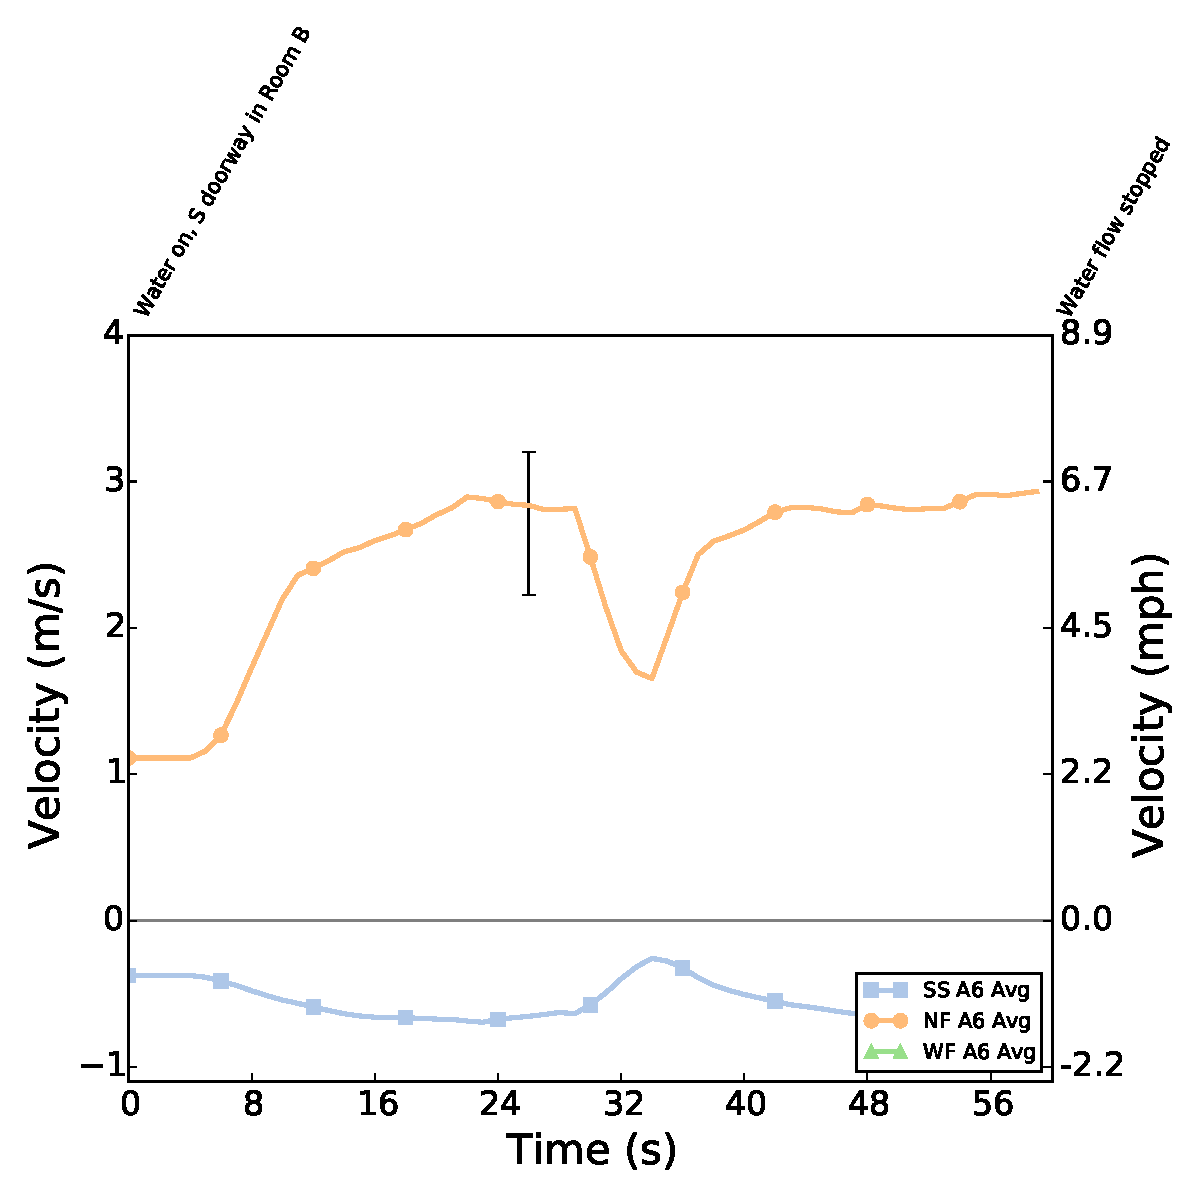
\includegraphics[width=\columnwidth]{../Figures/Plots/HOSE_IXXAXX_BDP_A6_stream_avgs}
	\caption{Average velocity through stairwell door during Test 16 for three hose stream patterns.}
	\label{fig:Test_33_BDP_A6_Avg_All}
\end{figure}
\FloatBarrier

\begin{figure}[!ht]
	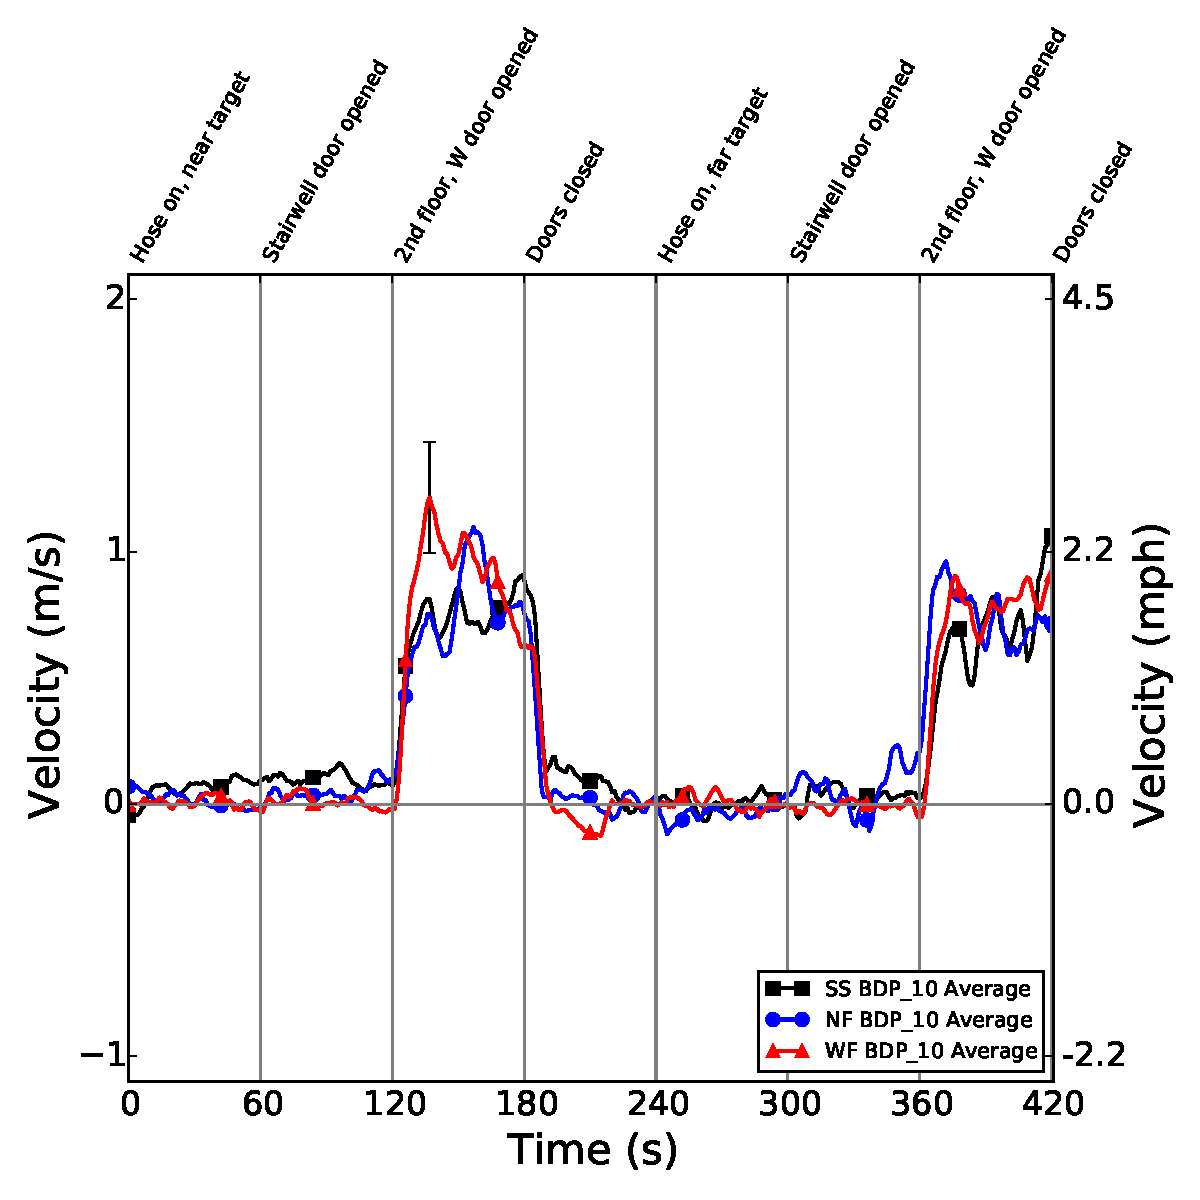
\includegraphics[width=\columnwidth]{../Figures/Plots/Test_17_West_063014_BDP_A10_stream_avgs}
	\caption{Average velocity through stairwell door during Test 17 for three hose stream patterns.}
	\label{fig:Test_17_BDP_A10_Avg_All}
	\end{figure}
\FloatBarrier

\begin{figure}[!ht]
	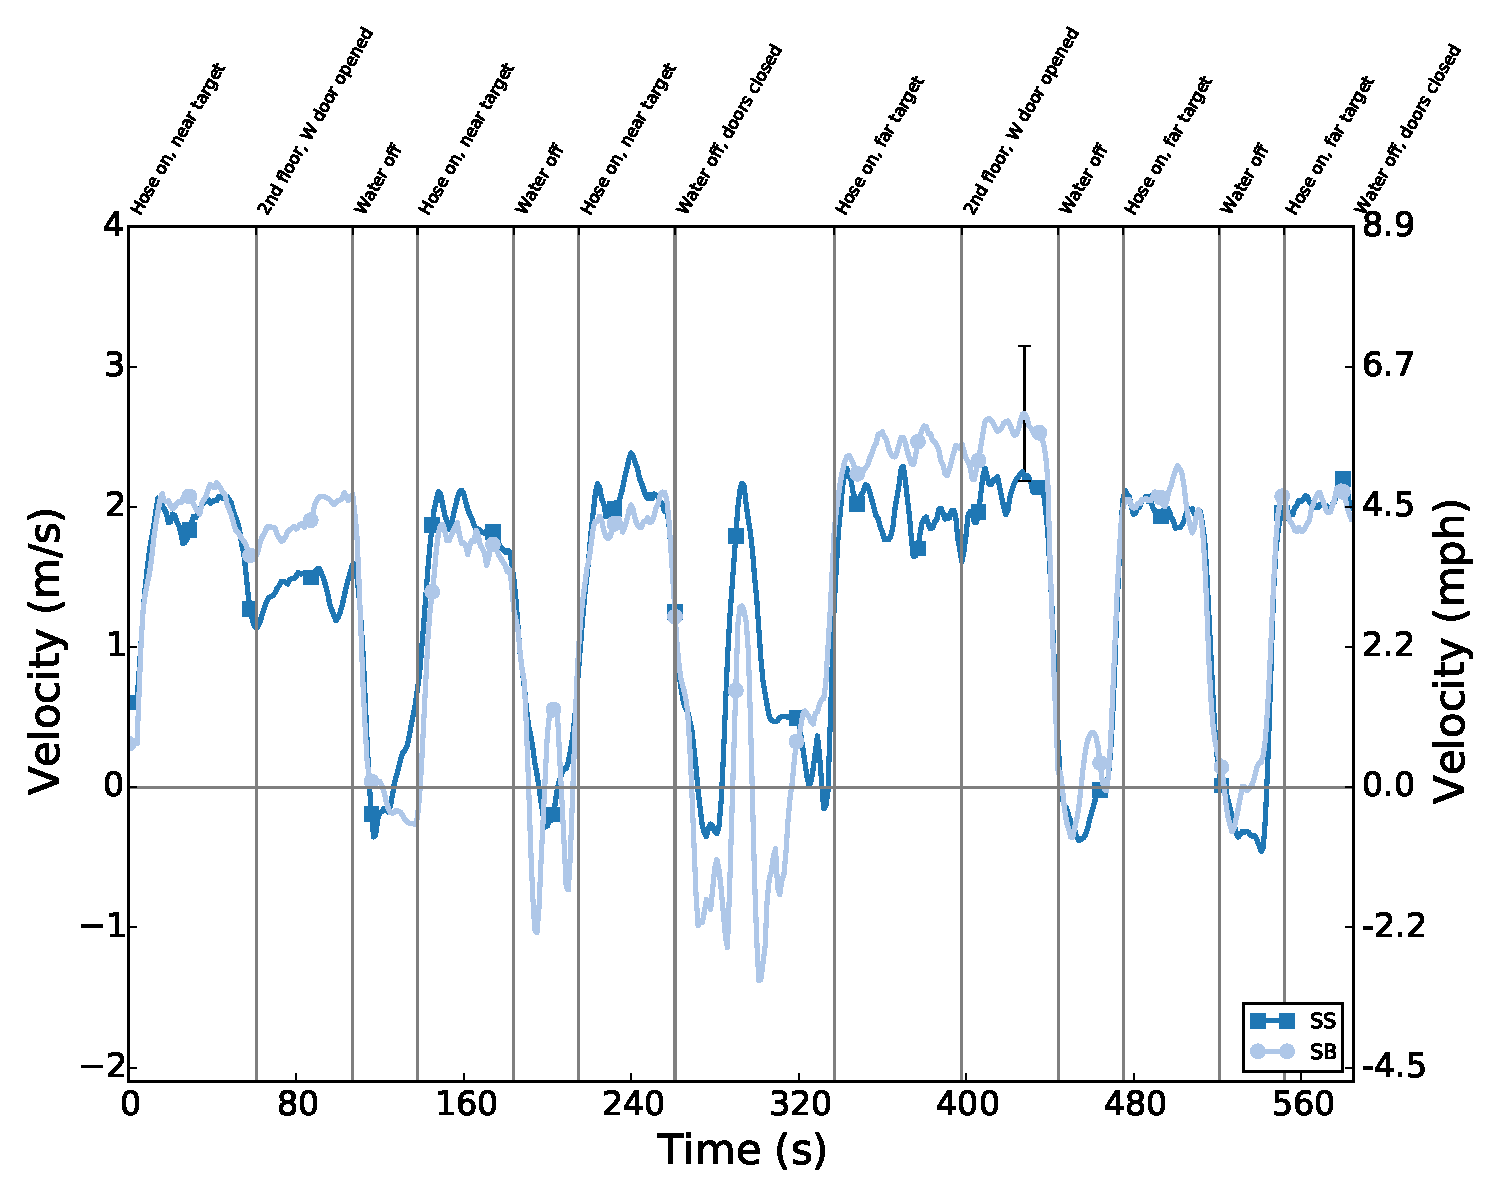
\includegraphics[width=\columnwidth]{../Figures/Plots/Test_70_West_101215_BDP_A10_stream_avgs}
	\caption{Average velocity through stairwell door during Test 70 for straight stream and smooth bore stream patterns.}
	\label{fig:Test_70_BDP_A10_Avg_All}
	\end{figure}
\FloatBarrier

\subsection{Handline Figures}
\label{sec:handline_figs}

\begin{figure}[!ht]
	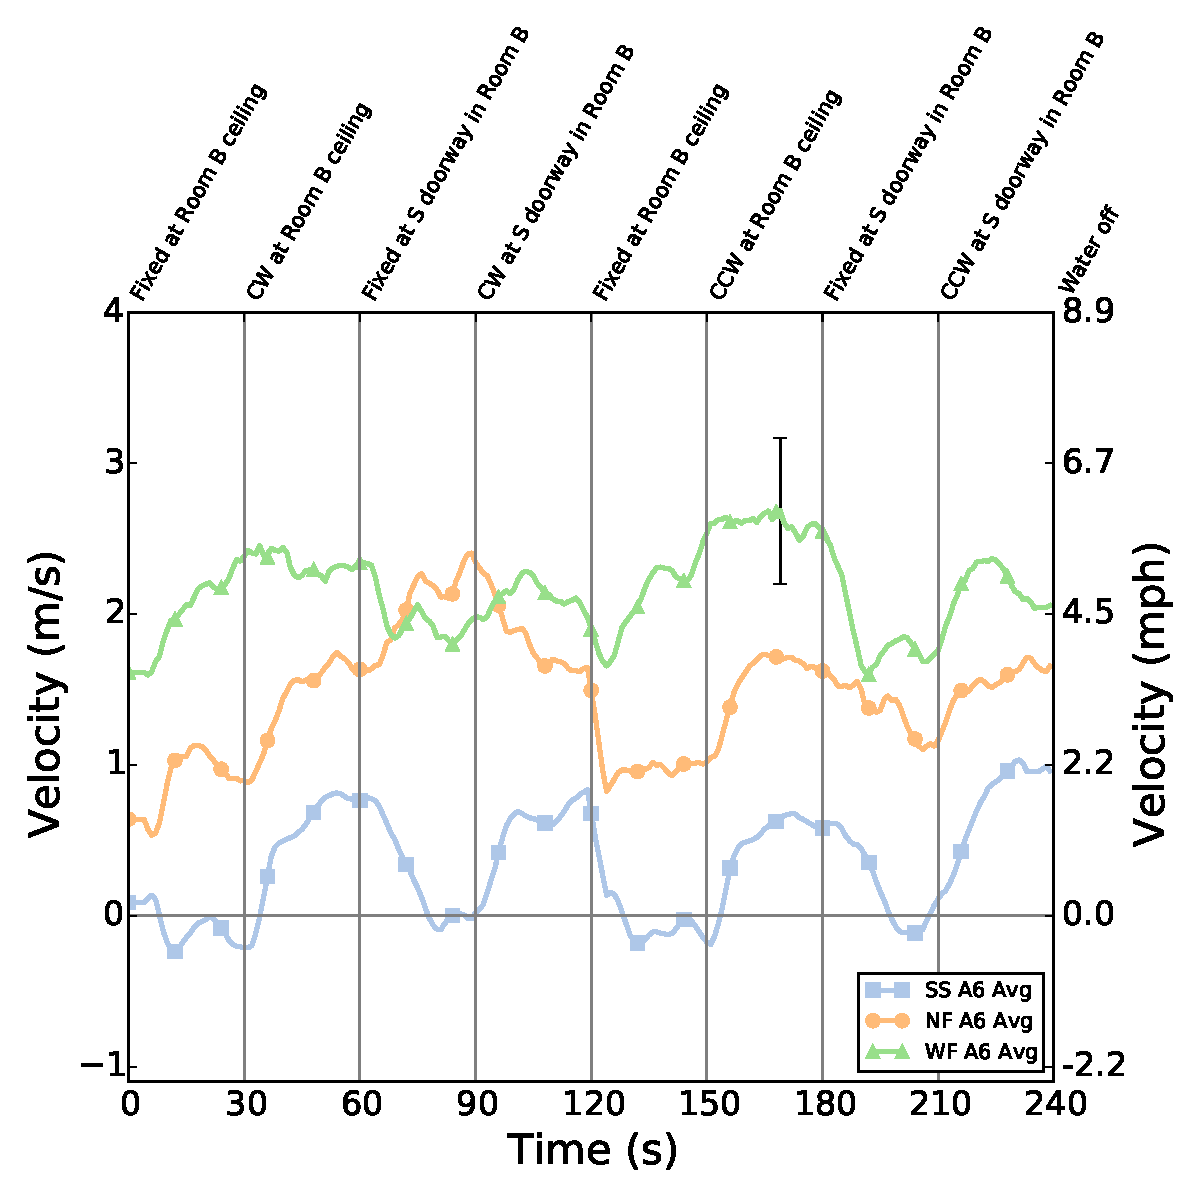
\includegraphics[width=\columnwidth]{../Figures/Plots/HOSE_IXAOXX_BDP_A6_stream_avgs}
	\caption{Average velocity through stairwell door during Test 16 for three hose stream patterns.}
	\label{fig:Test_34_BDP_A6_Avg_All}
\end{figure}
\FloatBarrier

\begin{figure}[!ht]
	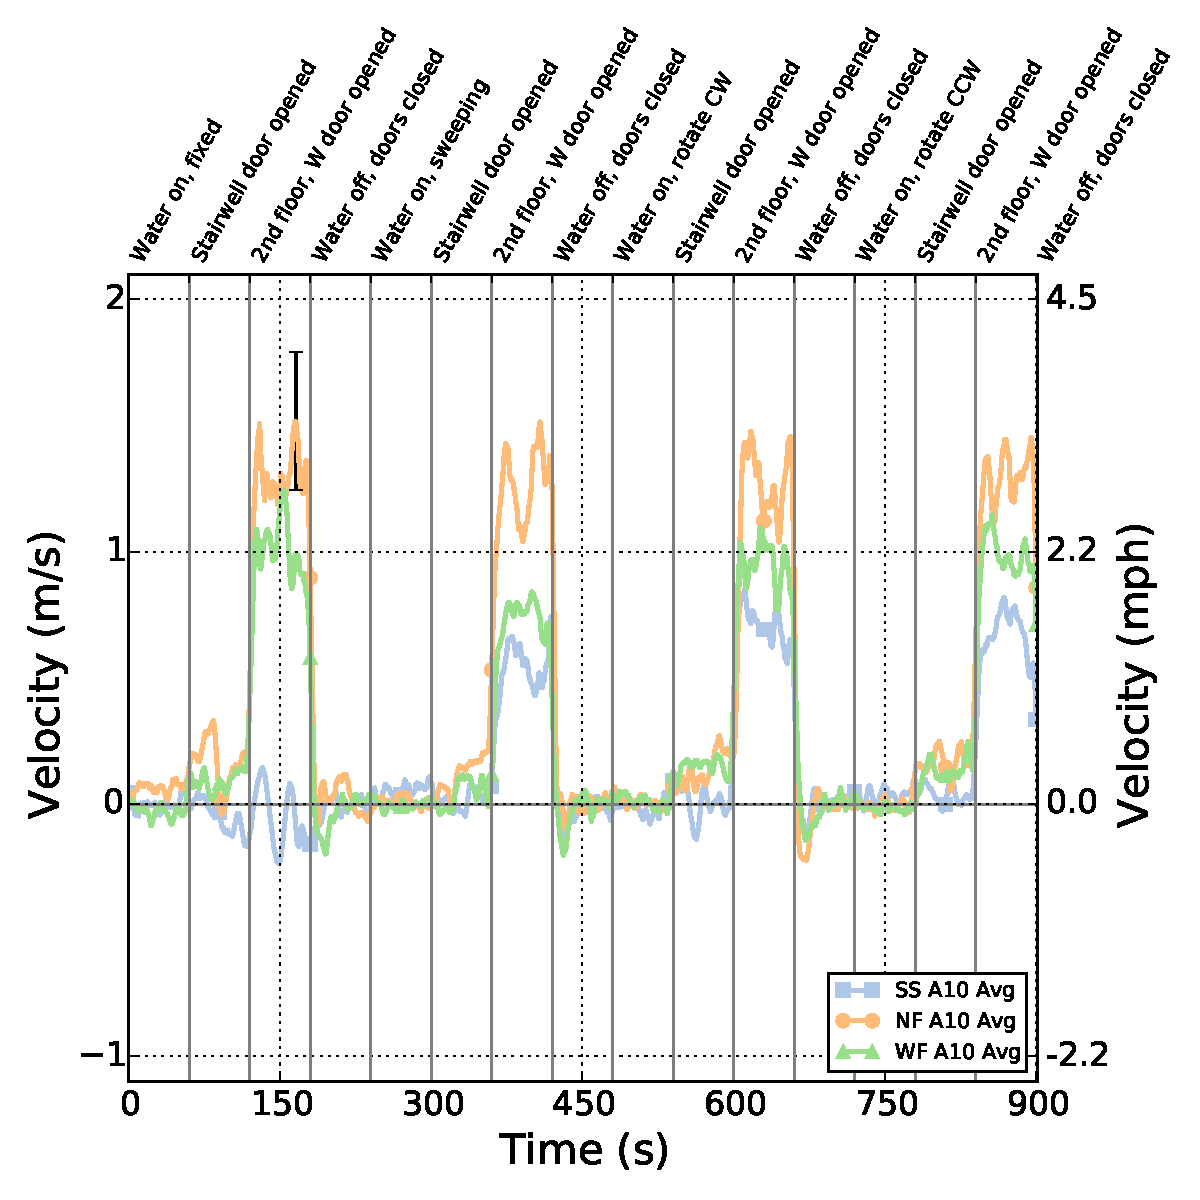
\includegraphics[width=\columnwidth]{../Figures/Plots/Test_19_West_063014_BDP_A10_stream_avgs}
	\caption{Average velocity through stairwell door during Test 19 for the three hose stream patterns.}
	\label{fig:Test_19_BDP_A10_Avg_All}
\end{figure}

\clearpage


\end{document}

